% =====================================================================
%  MẪU BÁO CÁO TIỂU LUẬN HỌC PHẦN HỌC MÁY - Nguyễn Tuấn Anh
%  ---------------------------------------------------------------------
%  Biên dịch bằng XeLaTeX (hoặc LuaLaTeX), chạy 2 lần để cập nhật mục lục.
%  Trên Overleaf: Menu > Compiler > XeLaTeX.
%  Trên máy:      latexmk -xelatex "Mau bao cao mon Hoc may.tex"
%
%  Cách dùng mẫu:
%   1. Sửa THÔNG TIN BÁO CÁO ở mục (A) bên dưới.
%   2. Viết nội dung vào các chương; xóa các đoạn \huongdan{...} khi hoàn thành.
%   3. Đặt hình vào thư mục images/ và thay các khung \khunghinh{...}
%      bằng \includegraphics[width=...]{ten_hinh.png}.
% =====================================================================
\documentclass[12pt,a4paper,oneside]{report}

% Cỡ chữ thân bài 13pt (theo quy định trình bày của bộ môn)
\makeatletter
\renewcommand\normalsize{%
  \@setfontsize\normalsize{13pt}{15.6pt}%
  \abovedisplayskip 12pt plus3pt minus7pt
  \belowdisplayskip \abovedisplayskip
  \abovedisplayshortskip 0pt plus3pt
  \belowdisplayshortskip 6.5pt plus3.5pt minus3pt}
\normalsize
\makeatother

% =====================================================================
%  (A) THÔNG TIN BÁO CÁO - SINH VIÊN SỬA TẠI ĐÂY
% =====================================================================
\newcommand{\truong}{TRƯỜNG ĐẠI HỌC CÔNG NGHỆ THÔNG TIN VÀ TRUYỀN THÔNG}
\newcommand{\khoa}{KHOA CÔNG NGHỆ THÔNG TIN}
\newcommand{\loaibaocao}{BÁO CÁO TIỂU LUẬN}
\newcommand{\hocphan}{Học máy}
\newcommand{\lophocphan}{KHMT K22}
\newcommand{\hocky}{Học kỳ 1, năm học 2026--2027}
\newcommand{\tendetai}{SO SÁNH CÁC THUẬT TOÁN HỌC MÁY TRUYỀN THỐNG TRONG DỰ ĐOÁN TƯƠNG TÁC THUỐC DỰA TRÊN CẤU TRÚC HÓA HỌC}
\newcommand{\tenbaitoan}{dự đoán tương tác thuốc} % dùng trong tên Chương 1 và 2
\newcommand{\giangvien}{TS. Nguyễn Tuấn Anh}  % thêm học hàm/học vị nếu cần
\newcommand{\nhom}{Nhóm 19}
\newcommand{\svAten}{Sùng A Khua}
\newcommand{\svAma}{DTC235160020}
\newcommand{\svBten}{Hoàng Bảo Ngọc}
\newcommand{\svBma}{DTC235160033}
\newcommand{\diadiem}{Thái Nguyên}
\newcommand{\thoigian}{tháng 11 năm 2026}

% ---------------- Trang giấy & phông chữ ----------------
\usepackage[a4paper,left=3cm,right=2cm,top=2.5cm,bottom=2.5cm,
            headheight=16pt,headsep=0.8cm]{geometry}
\usepackage{fontspec}
% Times New Roman; nếu máy không có thì dùng Liberation Serif (cùng thông số chữ)
\IfFontExistsTF{Times New Roman}{\setmainfont{Times New Roman}}{\setmainfont{Liberation Serif}}
\IfFontExistsTF{Consolas}{\setmonofont{Consolas}[Scale=0.9]}{\IfFontExistsTF{Courier New}{\setmonofont{Courier New}[Scale=0.9]}{\setmonofont{Liberation Mono}[Scale=0.9]}} % Overleaf khong co Consolas
\usepackage[vietnamese]{babel}
\usepackage{setspace}
\setstretch{1.3}
\setlength{\parindent}{1cm}
\setlength{\parskip}{6pt}
\usepackage{indentfirst}

% ---------------- Gói hỗ trợ ----------------
\usepackage{amsmath,amssymb}
\usepackage{graphicx}
\graphicspath{{images/}}
\usepackage{float}
\usepackage{array,booktabs,tabularx,multirow}
\usepackage{xltabular}
\setlength{\emergencystretch}{3em}
\renewcommand{\arraystretch}{1.25}
\usepackage[table]{xcolor}
\usepackage{tikz}
\usetikzlibrary{positioning,arrows.meta,calc,fit,backgrounds}
\usepackage{caption}
\captionsetup{labelsep=period,labelfont=bf,font=normalsize,skip=6pt}
\captionsetup[table]{position=top}
\usepackage{titlesec}
\usepackage{titletoc}
\usepackage[nottoc]{tocbibind}   % đưa danh mục hình, bảng, TLTK vào mục lục
\usepackage{enumitem}
\setlist{nosep,leftmargin=1.6cm}
\setlist[itemize]{label=\textendash}   % gạch đầu dòng thay cho chấm tròn
\usepackage{listings}
\usepackage{needspace}
\usepackage{cite}                % gộp trích dẫn: [4-6], [2, 4-6]
\usepackage{fancyhdr}
\usepackage[unicode]{hyperref}
\hypersetup{
  hidelinks,
  pdftitle={\tendetai},
  pdfauthor={\svAten, \svBten},
  pdfsubject={\loaibaocao\ học phần \hocphan},
  bookmarksnumbered=true,   % bookmark có số thứ tự chương, mục
  bookmarksopen=true,
  bookmarksopenlevel=0,
}
% Bookmark dạng "Chương 1. Tên chương", "1.1. Tên mục", "Phụ lục A. ..."
\newcommand{\bmchapname}{Chương}
\makeatletter
\newcommand*{\bm@prefix}{}
\let\bm@orig@writebookmark\Hy@writebookmark
\renewcommand*{\Hy@writebookmark}[5]{%
  \ifnum#4=0 \def\bm@prefix{\bmchapname\space}\else\def\bm@prefix{}\fi
  \bm@orig@writebookmark{#1}{#2}{#3}{#4}{#5}}
\renewcommand*{\Hy@numberline}[1]{\bm@prefix#1. }
\makeatother

% ---------------- Màu & định dạng mã nguồn ----------------
\definecolor{codebg}{RGB}{247,247,247}
\definecolor{codekw}{RGB}{0,51,153}
\definecolor{codecm}{RGB}{0,128,0}
\definecolor{codestr}{RGB}{163,21,21}
\definecolor{guide}{RGB}{110,110,110}
\lstdefinestyle{python}{
  language=Python,
  basicstyle=\ttfamily\small\setstretch{1.0},
  backgroundcolor=\color{codebg},
  keywordstyle=\color{codekw}\bfseries,
  commentstyle=\color{codecm}\itshape,
  stringstyle=\color{codestr},
  numbers=left, numberstyle=\tiny\color{guide}, numbersep=8pt,
  frame=single, rulecolor=\color{black!25},
  breaklines=true, showstringspaces=false, tabsize=4,
  xleftmargin=1.2em, framexleftmargin=1.2em,
  aboveskip=8pt, belowskip=8pt, columns=fullflexible, keepspaces=true,
}
\lstset{style=python}
\renewcommand{\lstlistingname}{Đoạn mã}
\renewcommand{\lstlistlistingname}{DANH MỤC ĐOẠN MÃ}

% ---------------- Tên gọi tiếng Việt ----------------
\addto\captionsvietnamese{%
  \renewcommand{\contentsname}{MỤC LỤC}%
  \renewcommand{\listfigurename}{DANH MỤC HÌNH ẢNH}%
  \renewcommand{\listtablename}{DANH MỤC BẢNG}%
  \renewcommand{\bibname}{TÀI LIỆU THAM KHẢO}%
  \renewcommand{\figurename}{Hình}%
  \renewcommand{\tablename}{Bảng}%
  \renewcommand{\chaptername}{Chương}%
  \renewcommand{\appendixname}{Phụ lục}%
}

% ---------------- Đầu trang & chân trang ----------------
\pagestyle{fancy}
\fancyhf{}
\fancyhead[L]{\small\itshape Báo cáo tiểu luận học phần \hocphan}
\fancyhead[R]{\small\itshape\nouppercase{\leftmark}}
\fancyfoot[C]{\thepage}
\renewcommand{\headrulewidth}{0.4pt}
\renewcommand{\chaptermark}[1]{\markboth{\chaptertitlename~\thechapter. #1}{}}
\fancypagestyle{plain}{\fancyhf{}\fancyfoot[C]{\thepage}\renewcommand{\headrulewidth}{0pt}}

% ---------------- Định dạng tiêu đề ----------------
% Chương: "CHƯƠNG 1" + tên chương in hoa - 14pt, đậm, căn giữa
\titleformat{\chapter}[display]
  {\filcenter\bfseries\fontsize{14}{18}\selectfont}
  {\MakeUppercase{\chaptertitlename}~\thechapter}{4pt}{\MakeUppercase}
\titlespacing*{\chapter}{0pt}{0pt}{18pt}
% Mục cấp 2: "1.1. Giới thiệu" - 14pt, đậm
\titleformat{\section}
  {\bfseries\fontsize{14}{18}\selectfont}{\thesection.}{0.5em}{}
\titlespacing*{\section}{0pt}{12pt}{6pt}
% Mục cấp 3: "1.1.1. Mục" - 13pt, đậm
\titleformat{\subsection}
  {\bfseries\fontsize{13}{17}\selectfont}{\thesubsection.}{0.5em}{}
\titlespacing*{\subsection}{0pt}{10pt}{6pt}
% Mục cấp 4: "1.1.1.1. Mục" - 13pt, đậm nghiêng
\setcounter{secnumdepth}{3}
\titleformat{\subsubsection}
  {\bfseries\itshape\fontsize{13}{17}\selectfont}{\thesubsubsection.}{0.5em}{}
\titlespacing*{\subsubsection}{0pt}{8pt}{4pt}

% ---------------- Mục lục & danh mục ----------------
\setcounter{tocdepth}{2}
\newcommand{\tocchapname}{Chương}
\titlecontents{chapter}[0pt]{\addvspace{6pt}\bfseries}
  {\tocchapname~\thecontentslabel.\enspace}{}{\titlerule*[0.6pc]{.}\contentspage}
\titlecontents{section}[1.5em]{}
  {\thecontentslabel.\enspace}{}{\titlerule*[0.6pc]{.}\contentspage}
\titlecontents{subsection}[3em]{}
  {\thecontentslabel.\enspace}{}{\titlerule*[0.6pc]{.}\contentspage}
\titlecontents{figure}[0pt]{}
  {\figurename~\thecontentslabel.\enspace}{}{\titlerule*[0.6pc]{.}\contentspage}
\titlecontents{table}[0pt]{}
  {\tablename~\thecontentslabel.\enspace}{}{\titlerule*[0.6pc]{.}\contentspage}

% ---------------- Lệnh tiện ích ----------------
% Chương không đánh số (Mở đầu, Kết luận...) vẫn có trong mục lục và đầu trang
\newcommand{\unnumberedchapter}[1]{%
  \chapter*{#1}\phantomsection\addcontentsline{toc}{chapter}{#1}\markboth{#1}{}}
% Ghi chú hướng dẫn (xóa khi viết xong)
\newcommand{\huongdan}[1]{{\color{guide}\itshape [Hướng dẫn: #1]}}
% Khung giữ chỗ cho hình: \khunghinh{rộng}{cao}{nội dung}
\newcommand{\khunghinh}[3]{%
  \begin{tikzpicture}
    \draw[dashed,thick,black!40,fill=black!3] (0,0) rectangle (#1,#2);
    \node[text width=0.8*#1,align=center,font=\itshape\color{guide}]
      at ($(0,0)!0.5!(#1,#2)$) {#3};
  \end{tikzpicture}}
% Dòng chấm để viết tay
% Ghi chú cần bổ sung (hiện màu đỏ, xóa khi đã điền)
\newcommand{\canbosung}[1]{{\color{red}[#1]}}
\newcommand{\dongcham}[1]{\par\noindent\foreach \i in {1,...,#1}{\makebox[\linewidth]{\dotfill}\\[4pt]}}

% =====================================================================
\begin{document}

% =====================================================================
%  TRANG BÌA
% =====================================================================
\begin{titlepage}
  \begin{tikzpicture}[remember picture,overlay]
    \draw[line width=2.2pt]
      ($(current page.north west)+(2.4cm,-1.6cm)$) rectangle
      ($(current page.south east)+(-1.4cm,1.6cm)$);
    \draw[line width=0.6pt]
      ($(current page.north west)+(2.55cm,-1.75cm)$) rectangle
      ($(current page.south east)+(-1.55cm,1.75cm)$);
  \end{tikzpicture}\par\vspace*{-\baselineskip}
  \centering\setstretch{1.2}
  {\fontsize{13}{18}\selectfont\bfseries \truong\par}
  {\fontsize{14}{18}\selectfont\bfseries \khoa\par}
  \vspace{2pt}\rule{0.35\textwidth}{0.8pt}\par
  \vspace{1.2cm}
  \IfFileExists{images/logo.png}
    {
\includegraphics[width=3.2cm]{logo.png}}
    {\khunghinh{3.2cm}{3.2cm}{Logo\\trường}}\par
  \vspace{1.2cm}
  {\fontsize{22}{28}\selectfont\bfseries \loaibaocao\par}
  \vspace{4pt}
  {\fontsize{16}{20}\selectfont\bfseries HỌC PHẦN: \MakeUppercase{\hocphan}\par}
  \vspace{1.2cm}
  {\fontsize{14}{18}\selectfont ĐỀ TÀI:\par}
  \vspace{4pt}
  {\fontsize{18}{26}\selectfont\bfseries \tendetai\par}
  \vfill
  \begin{tabular}{@{}l@{\hspace{0.6cm}}l@{}}
    \textbf{Giảng viên hướng dẫn:} & \giangvien \\
    \textbf{Lớp học phần:}         & \lophocphan \\
    \textbf{Nhóm thực hiện:}       & \nhom \\
                                   & \svAten\ -- \svAma \\
                                   & \svBten\ -- \svBma \\
  \end{tabular}\par
  \vspace{1.8cm}
  {\bfseries \diadiem, \thoigian\par}
\end{titlepage}

% =====================================================================
%  PHẦN ĐẦU (đánh số trang La Mã)
% =====================================================================
\pagenumbering{roman}
\pagestyle{plain}

% ---------------- Nhận xét của giảng viên ----------------
\chapter*{NHẬN XÉT CỦA GIẢNG VIÊN}
\noindent\textbf{1. Về hình thức và bố cục báo cáo:}
\dongcham{3}
\noindent\textbf{2. Về nội dung và kết quả thực hiện:}
\dongcham{5}
\noindent\textbf{3. Về tinh thần, thái độ làm việc của nhóm:}
\dongcham{3}
\noindent\textbf{4. Điểm đánh giá:}
\begin{center}
  \begin{tabular}{|>{\centering\arraybackslash}p{1.2cm}|p{5.5cm}|>{\centering\arraybackslash}p{2.6cm}|>{\centering\arraybackslash}p{2.6cm}|}
    \hline
    \rowcolor{black!8}\textbf{STT} & \textbf{Họ và tên sinh viên} & \textbf{Điểm số} & \textbf{Điểm chữ} \\ \hline
    1 & \svAten & & \\ \hline
    2 & \svBten & & \\ \hline
  \end{tabular}
\end{center}
\vspace{0.6cm}
\hfill
\begin{minipage}{0.45\textwidth}
  \centering
  \textit{\diadiem, ngày \dots\ tháng \dots\ năm \dots}\\
  \textbf{Giảng viên}\\
  \textit{(Ký và ghi rõ họ tên)}\\[1.8cm]
  \giangvien
\end{minipage}

% ---------------- Lời cam đoan ----------------
\unnumberedchapter{LỜI CAM ĐOAN}

Chúng em xin cam đoan báo cáo tiểu luận ``\textit{\tendetai}'' là kết quả
làm việc của nhóm dưới sự hướng dẫn của giảng viên \giangvien. Các số liệu,
kết quả thực nghiệm trình bày trong báo cáo là trung thực, được tạo ra từ
mã nguồn của nhóm và có thể chạy lại được. Mọi tài liệu, mã nguồn, dữ liệu
tham khảo đều được trích dẫn đầy đủ trong danh mục tài liệu tham khảo.

Khai báo sử dụng công cụ AI tạo sinh. Nhóm có sử dụng công cụ AI tạo sinh để
gợi ý và hỗ trợ lên ý tưởng trong quá trình thực hiện đề tài. Nhóm tự kiểm tra
lại toàn bộ kết quả, hiểu và giải thích được mọi nội dung đã nộp.

Nếu phát hiện có bất kỳ sự gian lận nào, chúng em xin hoàn toàn chịu trách
nhiệm trước giảng viên và nhà trường.

\vspace{0.6cm}
\hfill
\begin{minipage}{0.5\textwidth}
  \centering
  \textit{\diadiem, ngày \dots\ tháng \dots\ năm \dots}\\
  Nhóm sinh viên thực hiện\\
  \textit{(Ký và ghi rõ họ tên)}\\[2cm]
  \begin{tabular}{@{}c@{\hspace{1.5cm}}c@{}}
    \svAten & \svBten
  \end{tabular}
\end{minipage}

% ---------------- Lời cảm ơn ----------------
\unnumberedchapter{LỜI CẢM ƠN}

Chúng em xin chân thành cảm ơn thầy \giangvien{} đã giảng dạy học phần Học
máy, cung cấp bài giảng, mã nguồn mẫu và bộ tiêu chí đánh giá giúp nhóm định
hướng thực hiện đề tài. Chúng em cũng cảm ơn Khoa Công nghệ Thông tin, Trường
Đại học Công nghệ Thông tin và Truyền thông đã tạo điều kiện học tập, và cơ sở
dữ liệu DrugBank đã cấp quyền sử dụng dữ liệu cho mục đích học thuật.

Do thời gian và kiến thức về lĩnh vực dược học còn hạn chế, báo cáo không
tránh khỏi thiếu sót. Chúng em rất mong nhận được ý kiến đóng góp của thầy để
hoàn thiện đề tài.

\vspace{0.4cm}
\hfill\textit{Nhóm sinh viên thực hiện}

% ---------------- Bảng phân công ----------------
\unnumberedchapter{BẢNG PHÂN CÔNG NHIỆM VỤ}

Bảng~\ref{tab:phancong} liệt kê các nhiệm vụ chính của từng thành viên trong
quá trình thực hiện đề tài.

\begin{xltabular}{\textwidth}{|>{\centering\arraybackslash}p{1cm}|p{3.4cm}|X|>{\centering\arraybackslash}p{2.5cm}|}
\caption{Phân công nhiệm vụ}\label{tab:phancong}\\
  \hline
  \rowcolor{black!8}\textbf{STT} & \textbf{Họ và tên} & \textbf{Nhiệm vụ phụ trách} & \textbf{Mức độ hoàn thành} \\ \hline
\endfirsthead
\multicolumn{4}{l}{\textit{Bảng \thetable\ (tiếp theo)}}\\
  \hline
  \rowcolor{black!8}\textbf{STT} & \textbf{Họ và tên} & \textbf{Nhiệm vụ phụ trách} & \textbf{Mức độ hoàn thành} \\ \hline
\endhead
  1 & \svAten &
    -- Chọn đề tài; phát biểu bài toán, mục tiêu và chỉ số đánh giá\newline
    -- Trích xuất dữ liệu từ DrugBank; làm sạch và xử lý chất lượng dữ liệu\newline
    -- Xây dựng đặc trưng cặp thuốc, chia tập và quy trình huấn luyện\newline
    -- Huấn luyện, đánh giá và phân tích lỗi các mô hình\newline
    -- Viết báo cáo & \\ \hline
  2 & \svBten &
    -- Tìm, tổng hợp tài liệu tham khảo và các công trình liên quan\newline
    -- Khảo sát, thống kê mô tả dữ liệu và xây dựng tập mẫu âm\newline
    -- Tổng hợp cơ sở lý thuyết các thuật toán và các chỉ số đánh giá\newline
    -- Cải tiến đặc trưng, tối ưu siêu tham số và thử các mô hình tổ hợp\newline
    -- Viết báo cáo & \\ \hline
\end{xltabular}

% ---------------- Mục lục, danh mục ----------------
\begingroup\setstretch{1.1}\tableofcontents\endgroup
\listoffigures
\listoftables

% ---------------- Danh mục từ viết tắt ----------------
\unnumberedchapter{DANH MỤC TỪ VIẾT TẮT}

\begin{xltabular}{\textwidth}{|>{\centering\arraybackslash}p{1cm}|p{2.6cm}|X|}
  \hline
  \rowcolor{black!8}\textbf{STT} & \textbf{Viết tắt} & \textbf{Ý nghĩa} \\ \hline
\endfirsthead
  \hline
  \rowcolor{black!8}\textbf{STT} & \textbf{Viết tắt} & \textbf{Ý nghĩa} \\ \hline
\endhead
  1 & ADME & Absorption, Distribution, Metabolism, Excretion -- Hấp thu, phân bố, chuyển hóa, thải trừ \\ \hline
  2 & AUC & Area Under the Curve -- Diện tích dưới đường cong ROC \\ \hline
  3 & AUPR & Area Under the Precision--Recall curve -- Diện tích dưới đường cong Precision--Recall \\ \hline
  4 & CV & Cross-Validation -- Kiểm định chéo \\ \hline
  5 & CYP & Cytochrome P450 -- Hệ enzyme chuyển hóa thuốc ở gan \\ \hline
  6 & DDI & Drug--Drug Interaction -- Tương tác thuốc -- thuốc \\ \hline
  7 & ECFP & Extended-Connectivity Fingerprint -- Vân tay kết nối mở rộng (Morgan) \\ \hline
  8 & EDA & Exploratory Data Analysis -- Phân tích khám phá dữ liệu \\ \hline
  9 & ET & Extra Trees -- Cây ngẫu nhiên hóa cực độ \\ \hline
  10 & InChI & International Chemical Identifier -- Mã định danh hóa học quốc tế \\ \hline
  11 & IQR & Interquartile Range -- Khoảng tứ phân vị \\ \hline
  12 & LR & Logistic Regression -- Hồi quy Logistic \\ \hline
  13 & MACCS & Molecular ACCess System keys -- Bộ khóa cấu trúc MACCS \\ \hline
  14 & MI & Mutual Information -- Thông tin tương hỗ \\ \hline
  15 & PU & Positive--Unlabeled learning -- Học từ dữ liệu dương và chưa gán nhãn \\ \hline
  16 & RBF & Radial Basis Function -- Hàm nhân bán kính \\ \hline
  17 & RF & Random Forest -- Rừng ngẫu nhiên \\ \hline
  18 & ROC & Receiver Operating Characteristic \\ \hline
  19 & SMARTS & SMILES Arbitrary Target Specification -- Ngôn ngữ mô tả mẫu cấu trúc con \\ \hline
  20 & SMILES & Simplified Molecular-Input Line-Entry System -- Chuỗi biểu diễn cấu trúc phân tử \\ \hline
  21 & SVM & Support Vector Machine -- Máy vectơ hỗ trợ \\ \hline
  22 & TPSA & Topological Polar Surface Area -- Diện tích bề mặt phân cực \\ \hline
\end{xltabular}

% =====================================================================
%  PHẦN NỘI DUNG (đánh số trang Ả Rập)
% =====================================================================
\clearpage
\pagenumbering{arabic}
\pagestyle{fancy}

% =====================================================================
%  MỞ ĐẦU
% =====================================================================
\unnumberedchapter{MỞ ĐẦU}

\section*{1. Lý do chọn đề tài}
Tương tác thuốc -- thuốc (Drug--Drug Interaction, DDI) xảy ra khi một thuốc làm
thay đổi tác dụng hoặc độc tính của thuốc khác khi dùng đồng thời. Người cao
tuổi và bệnh nhân mắc nhiều bệnh mạn tính thường phải dùng nhiều thuốc cùng
lúc, nên nguy cơ gặp tương tác bất lợi rất lớn. Số cặp thuốc có thể kết hợp
tăng theo bình phương số thuốc, vì vậy không thể kiểm chứng tất cả bằng thực
nghiệm lâm sàng. Các cơ sở dữ liệu như DrugBank \cite{wishart2018} đã ghi nhận
hàng triệu tương tác, tạo điều kiện để học máy học ra quy luật từ cấu trúc hóa
học của thuốc và dự đoán các tương tác chưa được biết.

Về khoa học, đề tài cho phép so sánh có hệ thống các thuật toán học máy truyền
thống trên dữ liệu đặc trưng nhị phân, số chiều cao (vân tay phân tử). Về thực
tiễn, mô hình có thể dùng để sàng lọc sớm các cặp thuốc nghi ngờ tương tác,
hỗ trợ dược sĩ và bác sĩ ưu tiên kiểm tra.

\section*{2. Mục tiêu và nhiệm vụ}
Mục tiêu tổng quát: xây dựng và so sánh các mô hình học máy truyền
thống dự đoán một cặp thuốc có tương tác hay không, chỉ dựa trên cấu trúc hóa
học của hai thuốc.

Mục tiêu cụ thể:
\begin{itemize}
  \item Xây dựng bộ dữ liệu cặp thuốc sạch từ DrugBank 5.1, không trùng lặp, cân bằng lớp.
  \item Đạt ROC-AUC $\geq 0{,}85$ và F1 $\geq 0{,}80$ trên tập kiểm tra giữ lại;
        vượt rõ rệt mô hình cơ sở (ROC-AUC $=0{,}5$).
  \item Đánh giá khả năng tổng quát hóa khi gặp thuốc mới (chia theo nhóm thuốc).
\end{itemize}

Nhiệm vụ: (1) trích xuất, khảo sát, tiền xử lý dữ liệu; (2) biểu diễn
thuốc bằng vân tay phân tử; (3) huấn luyện, đánh giá các mô hình Logistic
Regression, Random Forest, SVM, XGBoost; (4) tối ưu siêu tham số, cải tiến và
lựa chọn mô hình cuối.

\section*{3. Đối tượng và phạm vi nghiên cứu}
\begin{itemize}
  \item Đối tượng: các cặp thuốc phân tử nhỏ đã được phê duyệt trong
        DrugBank 5.1 (bản xuất ngày 02/01/2025) và các mô hình phân loại nhị phân.
  \item Phạm vi: chỉ dự đoán có hay không tương tác (không dự
        đoán loại hoặc mức độ tương tác); chỉ dùng cấu trúc hóa học (SMILES),
        không dùng thông tin protein đích, tác dụng phụ; không xét thuốc sinh học.
\end{itemize}

\section*{4. Phương pháp thực hiện}
Dữ liệu được trích xuất từ file XML của DrugBank bằng Python (\texttt{lxml});
cấu trúc phân tử được xử lý và mã hóa bằng RDKit \cite{rdkit} thành vân tay
Morgan \cite{rogers2010} và MACCS \cite{durant2002}. Mẫu âm được tạo bằng
phương pháp lấy mẫu ngẫu nhiên các cặp chưa ghi nhận tương tác theo Ran
\textit{et al.} \cite{ran2022}. Các mô hình được cài đặt bằng Scikit-learn
\cite{pedregosa2011} và XGBoost \cite{chen2016}, đánh giá bằng kiểm định chéo
phân tầng 5-fold trên tập huấn luyện và một tập kiểm tra giữ lại.


\section*{5. Bố cục báo cáo}
Ngoài phần Mở đầu, Kết luận và Tài liệu tham khảo, báo cáo gồm
3 chương:
\begin{itemize}
  \item Chương 1. Tổng quan về tương tác thuốc và cơ sở lý thuyết:
        giải thích tương tác thuốc dưới góc nhìn tin hóa học -- từ cơ chế dược
        động học, dược lực học tới cách biểu diễn phân tử bằng SMILES, vân tay
        phân tử và đặc trưng hóa lý; phát biểu bài toán dưới góc nhìn học máy;
        trình bày nền tảng toán học của các thuật toán, các chỉ số đánh giá và
        tổng quan các công trình nghiên cứu liên quan.
  \item Chương 2. Phương pháp đề xuất và thiết kế quy trình thực
        nghiệm: trình bày chi tiết quy trình từ dữ liệu thô DrugBank
        $\rightarrow$ làm sạch, khảo sát, xây dựng mẫu âm $\rightarrow$ vectơ
        đặc trưng cặp thuốc $\rightarrow$ chia tập, lựa chọn thuật toán và cấu
        hình huấn luyện, đánh giá.
  \item Chương 3. Thực nghiệm, so sánh và đánh giá kết quả: kết quả
        của các mô hình ban đầu, phân tích lỗi và đặc trưng quan trọng, các cải
        tiến, bảng đối sánh công bằng giữa các thuật toán, khả năng tổng quát
        hóa và lựa chọn mô hình cuối cùng.
\end{itemize}

% =====================================================================
%  CHƯƠNG 1
% =====================================================================
\chapter{Tổng quan về tương tác thuốc và cơ sở lý thuyết}
\label{chap:tongquan}

\section{Tương tác thuốc -- thuốc}
\label{sec:ddi}

\subsection{Khái niệm và ý nghĩa}
Tương tác thuốc -- thuốc (Drug--Drug Interaction, DDI) là hiện tượng
tác dụng của một thuốc bị thay đổi khi dùng đồng thời với thuốc khác. Thay đổi
đó có thể là tăng tác dụng (dẫn tới tăng nguy cơ tác dụng không mong muốn),
giảm tác dụng (làm mất hiệu quả điều trị), hoặc xuất hiện một tác dụng mới
không có khi dùng riêng từng thuốc. Về mặt dữ liệu, mỗi tương tác được ghi
nhận dưới dạng một bộ ba (thuốc A, thuốc B, mô tả tương tác); đây chính
là định dạng mà cơ sở dữ liệu DrugBank \cite{wishart2018} sử dụng.

Vấn đề trở nên quan trọng vì hai lý do. Thứ nhất, hiện tượng đa trị liệu
(polypharmacy) -- một người bệnh dùng đồng thời nhiều thuốc -- ngày càng phổ
biến, đặc biệt ở người cao tuổi và người mắc nhiều bệnh mạn tính; một người
dùng $n$ thuốc sẽ có $\binom{n}{2}$ cặp thuốc cần xem xét. Thứ hai, số cặp
thuốc có thể có trong toàn bộ danh mục thuốc tăng theo bình phương số thuốc:
với $N$ thuốc, số cặp là $\binom{N}{2} = N(N-1)/2$. Với $N = 2.472$ thuốc trong
phạm vi khảo sát của báo cáo, con số này là hơn 3 triệu cặp -- không thể kiểm chứng toàn
bộ bằng thử nghiệm lâm sàng, vốn tốn kém và kéo dài. Nhiều tương tác chỉ được phát hiện sau khi thuốc đã lưu hành, thông qua khai
thác dữ liệu báo cáo tác dụng không mong muốn.
Khoảng trống giữa số cặp có thể có và số cặp đã được kiểm chứng chính là chỗ cho
các phương pháp tính toán (\textit{in silico}): mô hình học máy không thay thế
thử nghiệm, mà xếp hạng các cặp thuốc theo nguy cơ để ưu tiên kiểm chứng.

\subsection{Phân loại theo cơ chế}
Theo tài liệu dược lý học, tương tác thuốc được chia thành hai nhóm cơ chế lớn
(Hình~\ref{fig:cochecddi}).

(a) Tương tác dược động học (pharmacokinetic) là tương tác làm thay đổi
nồng độ của thuốc trong cơ thể, tức là ảnh hưởng tới quá trình cơ thể xử
lý thuốc. Quá trình này gồm bốn giai đoạn, thường viết tắt là ADME:
\begin{itemize}
  \item Hấp thu (Absorption): một thuốc có thể làm thay đổi độ pH dạ
        dày, tốc độ làm rỗng dạ dày hoặc tạo phức khó tan với thuốc kia, làm
        thay đổi lượng thuốc đi vào máu.
  \item Phân bố (Distribution): hai thuốc cùng gắn mạnh vào protein
        huyết tương có thể cạnh tranh vị trí gắn, làm thay đổi tỷ lệ thuốc ở
        dạng tự do -- dạng có hoạt tính.
  \item Chuyển hóa (Metabolism): đây là cơ chế được nghiên cứu nhiều
        nhất. Phần lớn thuốc phân tử nhỏ được chuyển hóa ở gan nhờ hệ enzyme
        cytochrome P450 (CYP). Một thuốc ức chế enzyme sẽ làm chậm
        chuyển hóa của thuốc dùng cùng (nồng độ thuốc kia tăng); ngược lại một
        thuốc cảm ứng enzyme làm tăng tốc chuyển hóa (nồng độ thuốc kia
        giảm). Vì nhiều thuốc cùng đi qua một số ít enzyme, cơ chế này tạo ra
        rất nhiều cặp tương tác.
  \item Thải trừ (Excretion): hai thuốc có thể cạnh tranh cùng một
        protein vận chuyển ở thận, làm thay đổi tốc độ đào thải.
\end{itemize}

(b) Tương tác dược lực học (pharmacodynamic) là tương tác xảy ra ở
đích tác dụng mà không nhất thiết làm thay đổi nồng độ thuốc: hai thuốc
tác động lên cùng một thụ thể hoặc cùng một hệ sinh lý có thể cộng hợp
(cùng chiều, làm tăng hiệu ứng), hiệp đồng (hiệu ứng lớn hơn tổng hai
hiệu ứng riêng) hoặc đối kháng (ngược chiều, làm giảm hiệu ứng).

\begin{figure}[H]
  \centering
  \begin{tikzpicture}[
      font=\small,
      goc/.style={draw,rounded corners=3pt,fill=black!10,align=center,
                  minimum height=0.85cm,text width=4.4cm,font=\small\bfseries},
      nhom/.style={draw,rounded corners=3pt,fill=black!4,align=center,
                   minimum height=0.95cm,text width=4.0cm},
      la/.style={draw,rounded corners=2pt,fill=white,anchor=west,
                 minimum height=0.72cm,text width=5.2cm,font=\footnotesize,
                 inner xsep=5pt},
      mui/.style={-{Stealth[length=2.2mm]},thick},
      noi/.style={thick}]
    \node[goc] (g) at (0,0.3) {Cơ chế tương tác thuốc};
    \node[nhom] (dd) at (-3.9,-1.3) {Dược động học\\[-2pt]\footnotesize(thay đổi nồng độ)};
    \node[nhom] (dl) at (3.9,-1.3) {Dược lực học\\[-2pt]\footnotesize(thay đổi đáp ứng)};
    \draw[noi] (g.south) -- ++(0,-0.35) coordinate (m);
    \draw[noi] (dd.north |- m) -- (dl.north |- m);
    \draw[mui] (dd.north |- m) -- (dd.north);
    \draw[mui] (dl.north |- m) -- (dl.north);
    % lá trái
    \node[la] (a1) at (-6.3,-2.75) {Hấp thu: pH, tạo phức};
    \node[la] (a2) at (-6.3,-3.70) {Phân bố: gắn protein huyết tương};
    \node[la] (a3) at (-6.3,-4.65) {Chuyển hóa: ức chế/cảm ứng CYP};
    \node[la] (a4) at (-6.3,-5.60) {Thải trừ: cạnh tranh vận chuyển};
    \draw[noi] (dd.south) -- (-3.9,-2.05) -- (-6.75,-2.05) -- (-6.75,-5.60);
    \foreach \y in {-2.75,-3.70,-4.65,-5.60} {\draw[mui] (-6.75,\y) -- ++(0.3,0);}
    % lá phải
    \node[la] (b1) at (1.4,-2.75) {Cộng hợp / hiệp đồng cùng đích};
    \node[la] (b2) at (1.4,-3.70) {Đối kháng tại thụ thể};
    \node[la] (b3) at (1.4,-4.65) {Tác động cùng một hệ sinh lý};
    \draw[noi] (dl.south) -- (3.9,-2.05) -- (0.95,-2.05) -- (0.95,-4.65);
    \foreach \y in {-2.75,-3.70,-4.65} {\draw[mui] (0.95,\y) -- ++(0.45,0);}
  \end{tikzpicture}
  \caption{Phân loại tương tác thuốc theo cơ chế}
  \label{fig:cochecddi}
\end{figure}

Cách phân loại này giải thích vì sao cấu trúc hóa học lại mang thông tin
dự đoán được. Việc một phân tử có bị một enzyme chuyển hóa hay không, có gắn
được vào một thụ thể hay không, phụ thuộc vào các mảnh cấu trúc (nhóm chức,
khung vòng) của phân tử đó. Hai thuốc có cấu trúc giống nhau thường đi qua cùng
các enzyme và gắn vào cùng các đích, nên thường có hồ sơ tương tác giống nhau --
đây chính là giả thuyết nền của Vilar \textit{et al.} \cite{vilar2012} và của
toàn bộ hướng dự đoán DDI dựa trên cấu trúc.

\subsection{Nguồn dữ liệu: cơ sở dữ liệu DrugBank}
DrugBank \cite{wishart2018} là cơ sở dữ liệu thuốc được dùng phổ biến nhất
trong các nghiên cứu dự đoán DDI. Mỗi bản ghi thuốc chứa định danh
(\texttt{DB} + 5 chữ số), tên, phân loại (\texttt{small molecule} hoặc
\texttt{biotech}), trạng thái phê duyệt, cấu trúc hóa học dưới dạng SMILES và
InChIKey, cùng danh sách tương tác với các thuốc khác kèm mô tả bằng văn bản.
Ba đặc điểm của dữ liệu DrugBank chi phối cách xây dựng bài toán học máy:
\begin{enumerate}
  \item Chỉ có nhãn dương. DrugBank ghi nhận các cặp có tương
        tác; không có cặp nào được khẳng định là ``không tương tác''. Đây là
        tình huống học từ dữ liệu dương và chưa gán nhãn
        (Mục~\ref{sec:ddihocmay}).
  \item Mỗi tương tác xuất hiện hai lần, ở bản ghi của thuốc A và của
        thuốc B, nên cần gộp về cặp không thứ tự.
  \item Thuốc sinh học thường không có SMILES. Các phân tử lớn
        (protein, kháng thể) không biểu diễn được bằng chuỗi SMILES ngắn gọn,
        nên hướng tiếp cận dựa trên cấu trúc chỉ áp dụng cho thuốc phân tử nhỏ.
\end{enumerate}

\section{Biểu diễn phân tử trong tin hóa học}
\label{sec:bieudienphantu}

Để đưa một phân tử thuốc vào mô hình học máy, cần chuyển nó qua ba mức biểu
diễn: chuỗi ký tự $\rightarrow$ đồ thị phân tử $\rightarrow$ vectơ số.

\subsection{Đồ thị phân tử}
Một phân tử được mô hình hóa tự nhiên bằng một đồ thị vô hướng
$G = (V, E)$, trong đó mỗi đỉnh $v \in V$ là một nguyên tử (mang các thuộc tính:
nguyên tố, số liên kết, điện tích hình thức, tính thơm, số hydro gắn kèm) và
mỗi cạnh $e \in E$ là một liên kết hóa học (mang thuộc tính: bậc liên kết đơn,
đôi, ba hoặc thơm). Theo quy ước của tin hóa học, các nguyên tử hydro thường
không được biểu diễn tường minh mà suy ra từ hóa trị, nên $|V|$ là số
nguyên tử nặng (heavy atoms). Mọi đặc trưng cấu trúc đều là hàm của đồ thị này.

\subsection{Chuỗi SMILES}
SMILES (Simplified Molecular-Input Line-Entry System) \cite{weininger1988} là
cách viết đồ thị phân tử thành một chuỗi ký tự ASCII bằng cách duyệt theo chiều
sâu trên đồ thị. Quy tắc chính:
\begin{itemize}
  \item Nguyên tử viết bằng ký hiệu nguyên tố: \texttt{C}, \texttt{N},
        \texttt{O}, \texttt{S}\dots; chữ thường (\texttt{c}, \texttt{n}) chỉ
        nguyên tử thơm.
  \item Liên kết đơn là mặc định (không viết), \texttt{=} là liên kết đôi,
        \texttt{\#} là liên kết ba.
  \item Nhánh đặt trong ngoặc đơn: \texttt{CC(=O)O} là axit axetic.
  \item Vòng được mở và đóng bằng cùng một chữ số: \texttt{c1ccccc1} là vòng
        benzen.
\end{itemize}
Hình~\ref{fig:cautrucsmiles} minh họa cấu trúc và chuỗi SMILES của bốn thuốc
quen thuộc. Một phân tử có thể viết bằng nhiều chuỗi SMILES khác nhau tùy điểm
bắt đầu duyệt; vì vậy các thư viện tin hóa học sinh ra SMILES chính tắc
(canonical SMILES) -- một chuỗi duy nhất cho mỗi phân tử, nhờ một thuật toán
đánh số nguyên tử xác định. Bên cạnh SMILES, InChIKey là mã băm 27 ký tự của định danh InChI, dùng để so khớp nhanh xem hai bản ghi có phải
cùng một cấu trúc hay không, nhờ đó phát hiện được các mã thuốc khác nhau cùng
một cấu trúc.

\begin{figure}[H]
  \centering
  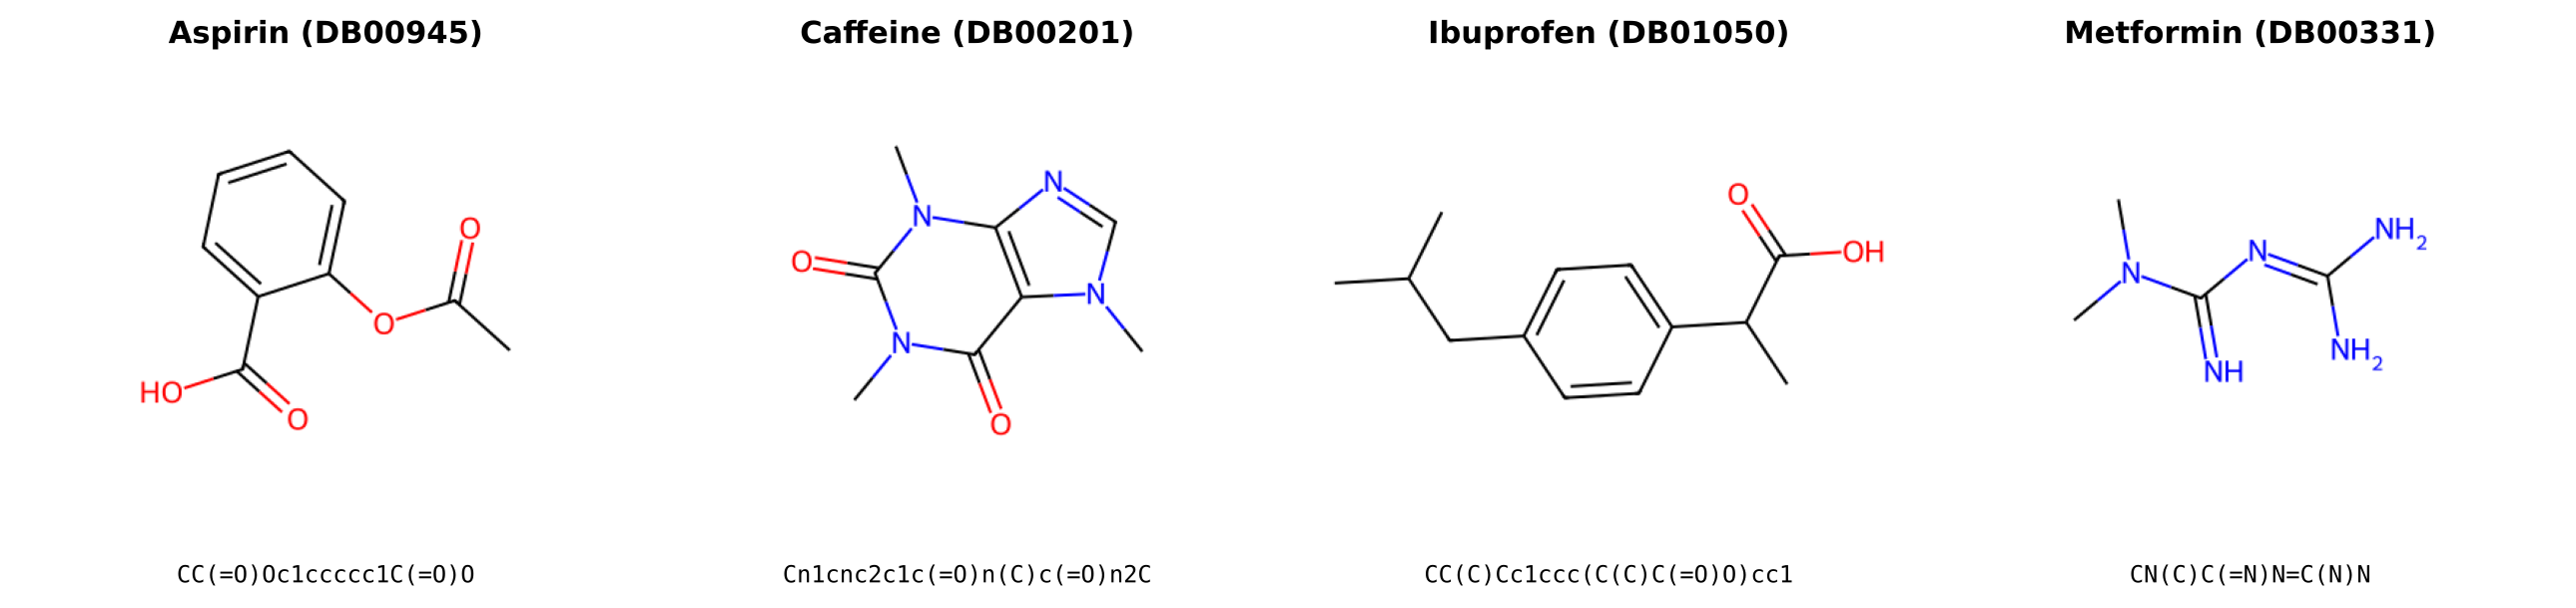
\includegraphics[width=\textwidth]{fig19_cau_truc_smiles.png}
  \caption{Cấu trúc hai chiều và chuỗi SMILES của bốn thuốc phân tử nhỏ}
  \label{fig:cautrucsmiles}
\end{figure}

\subsection{Chuẩn hóa cấu trúc}
Dữ liệu SMILES lấy từ cơ sở dữ liệu thực tế không đồng nhất, nên cần một bước
chuẩn hóa (standardization) trước khi tính đặc trưng. Các thao tác
thường dùng, đều có sẵn trong RDKit \cite{rdkit}:
\begin{itemize}
  \item Tách thành phần lớn nhất (largest fragment): nhiều thuốc được
        đăng ký dưới dạng muối (vd. hydrochloride) hoặc dạng ngậm nước, nên
        chuỗi SMILES gồm nhiều thành phần ngăn bởi dấu chấm. Ion đối và phân tử
        nước không quyết định hoạt tính nhưng làm vân tay của hai dạng muối của
        cùng một hoạt chất khác nhau, nên chỉ giữ thành phần lớn nhất.
  \item Chuẩn hóa nhóm chức và trung hòa điện tích: viết lại các nhóm
        chức tương đương về một dạng quy ước.
  \item Kiểm tra tính hợp lệ: chuỗi SMILES sai hóa trị sẽ không đọc
        được, cần loại bỏ.
  \item Loại phân tử quá nhỏ: các ion hoặc chất vô cơ chỉ có một vài
        nguyên tử nặng cho vân tay gần như toàn 0, không mang thông tin cấu
        trúc.
\end{itemize}
Bỏ qua bước này là một nguồn rò rỉ dữ liệu tinh vi: hai mã thuốc khác nhau
nhưng cùng một hoạt chất sẽ sinh ra hai mẫu có đặc trưng giống hệt nhau,
và nếu rơi vào hai tập huấn luyện/kiểm tra khác nhau thì kết quả đánh giá bị
thổi phồng.

\section{Vân tay phân tử và đặc trưng hóa lý}
\label{sec:vantay}

Vân tay phân tử (molecular fingerprint) là vectơ số -- thường là nhị
phân -- mã hóa sự có mặt của các mảnh cấu trúc trong phân tử. Đây là cầu nối
giữa đồ thị phân tử và mô hình học máy: sau bước này, mỗi thuốc trở thành một
điểm trong không gian nhiều chiều và mọi thuật toán phân loại thông thường đều
áp dụng được.

\subsection{Vân tay Morgan (ECFP)}
Vân tay Morgan, còn gọi là ECFP (Extended-Connectivity Fingerprint)
\cite{rogers2010}, là loại vân tay được dùng nhiều nhất hiện nay. Thuật toán
sinh vân tay gồm ba bước.

Bước 1 -- gán định danh ban đầu. Mỗi nguyên tử $v$ nhận một số nguyên
$id^{(0)}(v)$ băm từ các thuộc tính bất biến của nó: số nguyên tử (số hiệu
nguyên tố), số liên kết, số hydro gắn kèm, điện tích hình thức, khối lượng đồng
vị và việc nguyên tử có nằm trong vòng hay không.

Bước 2 -- lan truyền theo vòng lặp. Ở vòng lặp thứ $r = 1, 2, \dots, R$,
định danh của mỗi nguyên tử được cập nhật từ định danh của chính nó và của các
nguyên tử kề:
\begin{equation}
  id^{(r)}(v) = \mathrm{hash}\Big(\, id^{(r-1)}(v),\ \big\{\!\big\{\,
  (b_{vu},\, id^{(r-1)}(u)) : u \in \mathcal{N}(v) \big\}\!\big\} \Big),
  \label{eq:morgan}
\end{equation}
trong đó $\mathcal{N}(v)$ là tập nguyên tử kề $v$, $b_{vu}$ là bậc liên kết, và
$\{\!\{\cdot\}\!\}$ là đa tập được sắp xếp để kết quả không phụ thuộc thứ tự
duyệt. Sau vòng lặp thứ $r$, $id^{(r)}(v)$ mã hóa toàn bộ vùng lân cận bán kính
$r$ quanh nguyên tử $v$ (Hình~\ref{fig:morganbankinh}). Công thức~\eqref{eq:morgan}
chính là một dạng của thuật toán làm mới nhãn Weisfeiler--Lehman, và cũng là ý
tưởng mà các mạng nơ-ron đồ thị hiện đại kế thừa.

Bước 3 -- băm vào vectơ độ dài cố định. Tập hợp tất cả các định danh
$\{ id^{(r)}(v) : v \in V,\ 0 \le r \le R \}$ được băm vào $L$ vị trí
(thường $L = 1.024$):
\begin{equation}
  x_j = \mathbb{1}\big[\, \exists\, v, r:\ id^{(r)}(v) \bmod L = j \,\big],
  \qquad j = 0, 1, \dots, L-1 .
  \label{eq:bang}
\end{equation}
Nếu giữ nguyên số lần xuất hiện thay vì chỉ 0/1, ta có vân tay dạng đếm
(count fingerprint).

\begin{figure}[H]
  \centering
  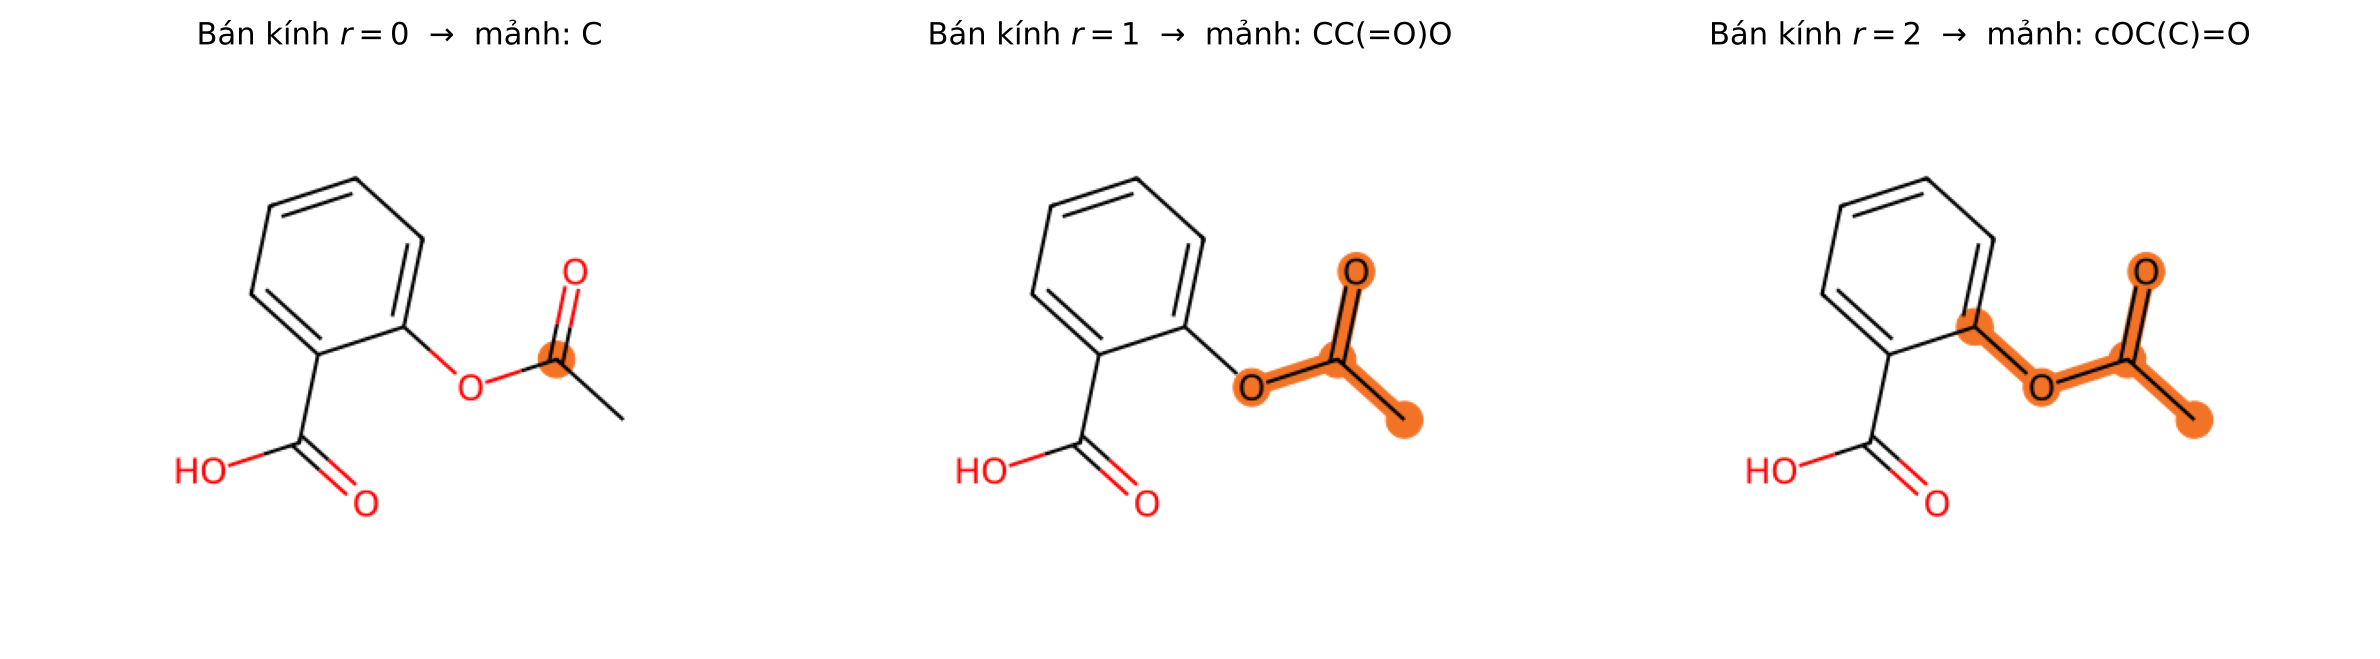
\includegraphics[width=\textwidth]{fig20_morgan_ban_kinh.png}
  \caption{Vùng lân cận bán kính $r = 0, 1, 2$ quanh một nguyên tử của Aspirin
           và mảnh cấu trúc tương ứng được mã hóa thành một bit}
  \label{fig:morganbankinh}
\end{figure}

Hai tham số quan trọng là bán kính $R$ và độ dài $L$. Bán kính $R = 2$ (tương
ứng ECFP4, vì đường kính bằng 4 liên kết) là lựa chọn phổ biến: đủ lớn để mô tả
một nhóm chức cùng môi trường xung quanh, nhưng chưa lớn đến mức mỗi mảnh gần
như đặc trưng cho riêng một phân tử. Độ dài $L$ quyết định mức độ
va chạm băm (hash collision): vì số mảnh cấu trúc có thể có lớn hơn $L$
rất nhiều, hai mảnh khác nhau có thể cùng bật một bit. Đây là cái giá phải trả
để có vectơ độ dài cố định, và cũng là lý do một bit Morgan không có ý nghĩa hóa
học duy nhất -- khi diễn giải độ quan trọng đặc trưng, chỉ có thể nói về mảnh hay gặp nhất làm bật
bit đó.

\subsection{Bộ khóa MACCS}
Khác với Morgan sinh mảnh tự động, MACCS \cite{durant2002} là một bộ
166 khóa cấu trúc định sẵn do chuyên gia thiết kế. Mỗi khóa là một câu
hỏi có/không dưới dạng mẫu SMARTS, ví dụ ``phân tử có chứa nguyên tử thơm
không'', ``có liên kết lưu huỳnh -- nitơ không''. Cài đặt trong RDKit trả về
vectơ 167 bit (bit 0 không dùng). Hình~\ref{fig:maccskhoa} minh họa hai khóa
được bật trên hai phân tử.

\begin{figure}[H]
  \centering
  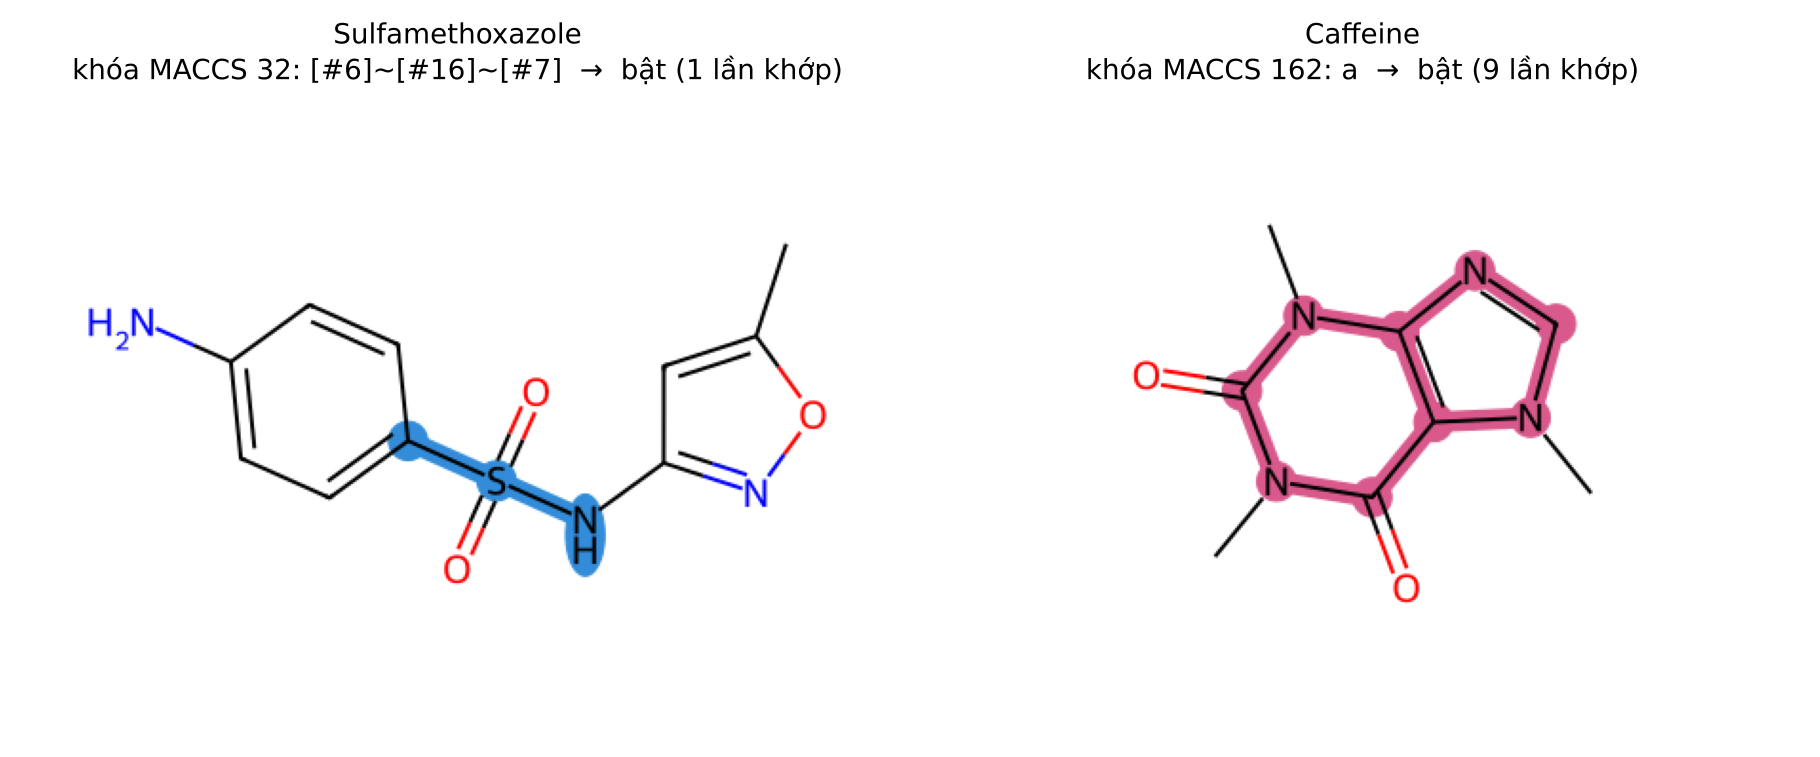
\includegraphics[width=\textwidth]{fig21_maccs_khoa.png}
  \caption{Hai khóa MACCS và các mảnh con khớp mẫu SMARTS tương ứng}
  \label{fig:maccskhoa}
\end{figure}

So sánh hai loại vân tay: MACCS ngắn, dễ diễn giải (mỗi bit có ý nghĩa hóa học
rõ ràng, không có va chạm băm) nhưng độ phân giải thấp -- nhiều phân tử khác
nhau có thể cùng một vectơ MACCS; Morgan dài hơn, thưa hơn, mô tả chi tiết hơn
nhưng khó diễn giải. Hai loại bổ sung cho nhau nên thường được dùng kết hợp.

\subsection{Độ tương đồng Tanimoto}
Để đo mức giống nhau giữa hai phân tử qua vân tay nhị phân $\mathbf{a}$ và
$\mathbf{b}$, chỉ số chuẩn là hệ số Tanimoto (còn gọi là Jaccard):
\begin{equation}
  T(\mathbf{a}, \mathbf{b}) = \frac{|\mathbf{a} \cap \mathbf{b}|}
  {|\mathbf{a}| + |\mathbf{b}| - |\mathbf{a} \cap \mathbf{b}|}
  = \frac{\sum_j a_j b_j}{\sum_j a_j + \sum_j b_j - \sum_j a_j b_j}
  \in [0, 1],
  \label{eq:tanimoto}
\end{equation}
bằng số bit cùng bật chia cho số bit bật ở ít nhất một trong hai vectơ. Tanimoto
được ưa dùng hơn khoảng cách Euclid vì vân tay rất thưa: với hai vectơ mà đa số
bit đều bằng 0, các bit cùng tắt không mang thông tin, và Tanimoto -- khác với
Euclid hay Hamming -- bỏ qua chúng. Trên vân tay 2D, Tanimoto là mốc chuẩn
trong sàng lọc ảo nhờ tính đơn giản và hiệu quả thực nghiệm.

Hình~\ref{fig:tanimoto} cho thấy chỉ số này hoạt động đúng như mong đợi trên các
thuốc quen thuộc: các cặp cùng nhóm cấu trúc (Aspirin -- Salicylic acid 0,46;
Ibuprofen -- Naproxen 0,42; Caffeine -- Theophylline 0,47) có Tanimoto cao hơn
hẳn các cặp khác nhóm (dưới 0,21). Cần lưu ý ngưỡng: trong tin hóa học, Tanimoto
khoảng 0,4--0,5 trên vân tay Morgan đã được xem là ``tương đồng đáng kể'', chứ
không phải 0,9 như trực giác thông thường về tỷ lệ phần trăm.

\begin{figure}[H]
  \centering
  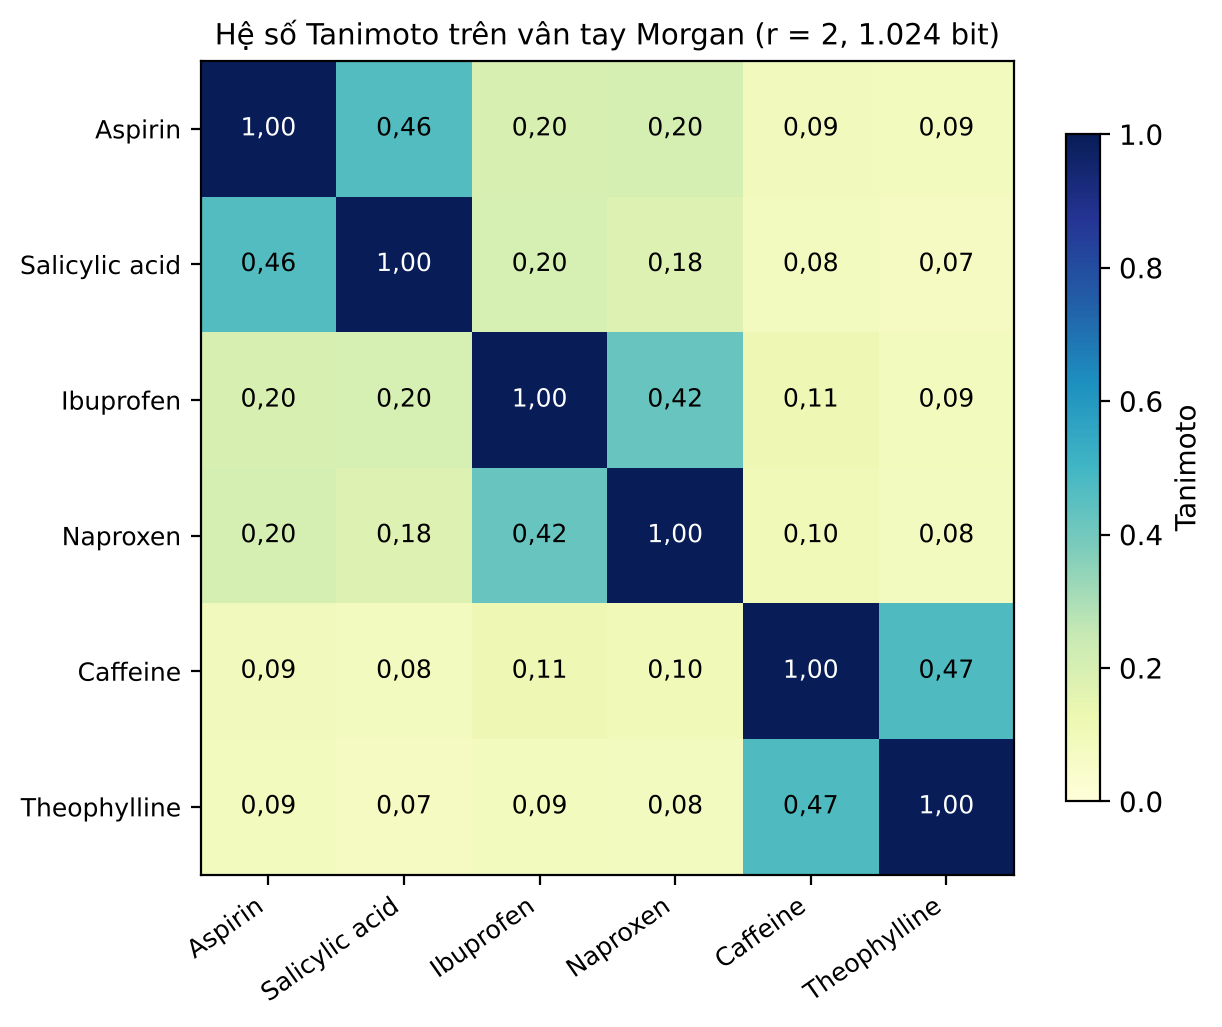
\includegraphics[width=0.78\textwidth]{fig22_tanimoto.png}
  \caption{Ma trận độ tương đồng Tanimoto giữa sáu thuốc thuộc ba nhóm cấu trúc}
  \label{fig:tanimoto}
\end{figure}

\subsection{Đặc trưng mô tả hóa lý}
Ngoài vân tay, mỗi phân tử còn được mô tả bằng các đại lượng hóa lý
(physicochemical descriptors) tính trực tiếp từ đồ thị phân tử. Các đại lượng
thường dùng (Bảng~\ref{tab:hoaly}) đều liên quan tới quá trình ADME
nói ở Mục~\ref{sec:ddi}: khối lượng phân tử và số nguyên tử nặng phản ánh kích
thước; LogP (hệ số phân bố octanol/nước) phản ánh độ ưa béo, quyết định khả năng
thấm qua màng; TPSA (diện tích bề mặt phân cực) và số nhóm cho/nhận liên kết
hydro liên quan tới khả năng hấp thu; số liên kết quay tự do phản ánh độ mềm dẻo
của phân tử. Nhóm đại lượng này cũng là cơ sở của
``quy tắc năm'' mô tả khoảng giá trị thường gặp ở các thuốc uống được.

\begin{table}[H]
  \centering
  \caption{Các đặc trưng mô tả hóa lý thường dùng}
  \label{tab:hoaly}
  \small
  \begin{tabularx}{\textwidth}{>{\raggedright\arraybackslash}p{3.0cm}
                               >{\raggedright\arraybackslash}p{3.4cm} X}
    \toprule
    \textbf{Đại lượng} & \textbf{Ý nghĩa} & \textbf{Liên quan tới tương tác thuốc} \\
    \midrule
    \texttt{mol\_wt} (Da) & Khối lượng phân tử & Kích thước phân tử, ảnh hưởng tới hấp thu và phân bố \\
    \texttt{logp} & Độ ưa béo (Crippen LogP) & Khả năng thấm qua màng; thuốc rất ưa béo hay được chuyển hóa qua gan \\
    \texttt{tpsa} (Å$^2$) & Diện tích bề mặt phân cực & Khả năng hấp thu qua đường tiêu hóa \\
    \texttt{hbd}, \texttt{hba} & Số nhóm cho / nhận liên kết hydro & Khả năng gắn vào thụ thể và protein huyết tương \\
    \texttt{rot\_bonds} & Số liên kết quay tự do & Độ mềm dẻo của phân tử khi gắn vào đích \\
    \texttt{rings}, \texttt{arom\_rings} & Số vòng, số vòng thơm & Khung cấu trúc; vòng thơm hay gặp ở cơ chất của enzyme chuyển hóa \\
    \texttt{heavy\_atoms} & Số nguyên tử nặng & Kích thước đồ thị phân tử \\
    \bottomrule
  \end{tabularx}
\end{table}

Khác với vân tay nhị phân, các đại lượng này là số thực có thang đo rất khác
nhau (khối lượng phân tử hàng trăm, LogP khoảng $-5$ đến $5$), nên khi dùng với
mô hình tuyến tính hoặc SVM cần chuẩn hóa; mô hình cây không cần vì chỉ so sánh
ngưỡng.

\section{Bài toán dự đoán tương tác thuốc dưới góc nhìn học máy}
\label{sec:ddihocmay}

\subsection{Phát biểu dưới dạng dự đoán liên kết}
Gọi $\mathcal{D}$ là tập thuốc. Tập các tương tác đã biết tạo thành một đồ thị
vô hướng $\mathcal{G} = (\mathcal{D}, \mathcal{E})$, trong đó cạnh
$\{A, B\} \in \mathcal{E}$ nghĩa là cặp $(A, B)$ có tương tác đã ghi nhận. Dự
đoán DDI vì vậy là một bài toán dự đoán liên kết (link prediction): cho
một cặp chưa có cạnh, ước lượng khả năng cạnh đó tồn tại. Hai hướng khai thác
bài toán này khác nhau căn bản:
\begin{itemize}
  \item Hướng dựa trên đồ thị tương tác: dùng chính cấu trúc của
        $\mathcal{G}$ (số láng giềng chung, nhúng đỉnh\dots) làm đặc trưng. Ưu
        điểm là chính xác cao với thuốc đã có nhiều tương tác; nhược điểm là
        không áp dụng được cho thuốc mới -- đỉnh chưa có cạnh nào.
  \item Hướng dựa trên thuộc tính thuốc: mỗi thuốc
        được mô tả bằng vectơ đặc trưng $\phi(A) \in \mathbb{R}^{d}$ tính từ cấu
        trúc hóa học, và mô hình học hàm $f(\phi(A), \phi(B)) \to [0,1]$. Hướng
        này về nguyên tắc áp dụng được cho thuốc mới, miễn là biết cấu trúc.
\end{itemize}
Bài toán có thể phát biểu ở dạng nhị phân (có hay không có tương tác) hoặc đa
lớp (dự đoán loại tương tác); Mục~\ref{sec:lienquan} điểm qua cả hai hướng.

\subsection{Tính đối xứng của cặp không thứ tự}
Cặp thuốc là một cặp không thứ tự: $(A, B)$ và $(B, A)$ là cùng một đối
tượng. Hàm dự đoán vì vậy phải đối xứng:
\begin{equation}
  f(\phi(A), \phi(B)) = f(\phi(B), \phi(A)) \qquad \forall A, B .
  \label{eq:doixung}
\end{equation}
Có ba cách thường dùng để tạo vectơ đặc trưng cho cặp từ vectơ của từng thuốc:
\begin{enumerate}
  \item Ghép nối $[\phi(A) \,\|\, \phi(B)]$, số chiều $2d$. Giữ nguyên
        mọi thông tin nhưng không đối xứng: phải quy ước một thứ tự (vd.
        mã thuốc nhỏ hơn đứng trước), và mô hình có thể học cả thông tin vô tình
        nằm trong quy ước đó.
  \item Toán tử đối xứng: tổng $\phi(A) + \phi(B)$, tích Hadamard
        $\phi(A) \odot \phi(B)$, hoặc trị tuyệt đối của hiệu
        $|\phi(A) - \phi(B)|$; số chiều $d$. Thỏa mãn~\eqref{eq:doixung} theo
        thiết kế và giảm một nửa số chiều, nhưng mất một phần thông tin (vd. với
        phép tổng, giá trị 1 không phân biệt được ``mảnh này chỉ có ở $A$'' với
        ``chỉ có ở $B$''). Ran \textit{et al.} \cite{ran2022} so sánh đúng các
        toán tử này.
  \item Đối xứng hóa ở bước dự đoán: giữ ghép nối khi huấn luyện, khi
        dự đoán thì lấy trung bình $\tfrac{1}{2}[f(\phi_A, \phi_B) +
        f(\phi_B, \phi_A)]$; hoặc huấn luyện trên cả hai thứ tự (nhân đôi dữ
        liệu).
\end{enumerate}

\subsection{Vấn đề mẫu âm: học từ dữ liệu dương và chưa gán nhãn}
Như đã nêu, cơ sở dữ liệu chỉ cung cấp các cặp dương. Đây là tình huống
học từ dữ liệu dương và chưa gán nhãn (Positive--Unlabeled learning): tập
còn lại là hỗn hợp của các cặp thực sự không tương tác và các cặp có
tương tác nhưng chưa được phát hiện. Giải pháp phổ biến nhất là giả thiết ``thế giới đóng'': lấy ngẫu nhiên một phần các
cặp chưa ghi nhận làm mẫu âm. Giả thiết này kéo theo hai hệ quả phải kiểm soát:
\begin{itemize}
  \item Nhiễu nhãn: một tỷ lệ mẫu âm thực chất là dương chưa biết. Mô
        hình học được vẫn hữu ích cho mục tiêu xếp hạng, nhưng các chỉ số tuyệt
        đối bị ước lượng thiên lệch.
  \item Thiên lệch theo bậc (degree bias): trong đồ thị $\mathcal{G}$,
        các thuốc được nghiên cứu kỹ có rất nhiều cạnh. Nếu lấy mẫu âm ngẫu
        nhiên đều, các thuốc ``ít tương tác'' sẽ xuất hiện nhiều một cách bất
        thường ở lớp âm. Mô hình khi đó có thể đạt điểm cao chỉ bằng cách nhận
        ra độ phổ biến của từng thuốc, thay vì học quan hệ giữa hai cấu
        trúc. Đây là một dạng ``lối tắt'' (shortcut learning) và là một trong
        những điểm yếu ít được báo cáo của các nghiên cứu DDI.
\end{itemize}

\subsection{Rò rỉ dữ liệu và các chế độ chia tập}
Vì mỗi thuốc xuất hiện trong rất nhiều cặp, cách chia tập quyết định ý nghĩa của
kết quả đánh giá. Ba chế độ thường được phân biệt trong tài liệu:
\begin{itemize}
  \item S0 (chia theo cặp, ``thuốc đã biết''): chia ngẫu nhiên tập cặp.
        Hầu như mọi thuốc trong tập kiểm tra đều đã xuất hiện trong tập huấn
        luyện. Kết quả phản ánh khả năng ``điền vào chỗ trống'' của ma trận
        tương tác.
  \item S1 (một thuốc mới): cặp kiểm tra gồm một thuốc đã biết và một
        thuốc chưa từng xuất hiện khi huấn luyện.
  \item S2 (hai thuốc mới): cả hai thuốc đều chưa từng xuất hiện. Đây
        là chế độ khó nhất và gần với tình huống sàng lọc thuốc mới phát triển.
\end{itemize}
Điểm số luôn giảm dần theo thứ tự S0 $>$ S1 $>$ S2; một báo cáo chỉ nêu kết quả
S0 sẽ cho ấn tượng lạc quan quá mức. Ngoài ra còn ba nguồn rò rỉ cụ thể cần
chặn: (i) cùng một tương tác xuất hiện ở cả hai chiều A--B và B--A; (ii) hai mã
thuốc trùng cấu trúc rơi vào hai tập khác nhau; (iii) dùng bậc của thuốc
(số tương tác) làm đặc trưng -- đại lượng này tính trực tiếp từ nhãn nên là rò
rỉ hiển nhiên.

\section{Cơ sở toán học của các thuật toán sử dụng}
\label{sec:cosotoan}

Mục này trình bày nền tảng toán học của các thuật toán phân loại thường dùng
với dữ liệu dạng bảng.
Ký hiệu chung: tập huấn luyện $\mathcal{S} = \{(\mathbf{x}_i, y_i)\}_{i=1}^{n}$
với $\mathbf{x}_i \in \mathbb{R}^{d}$ và $y_i \in \{0, 1\}$.

\subsection{Khung chung: cực tiểu rủi ro thực nghiệm}
Mọi thuật toán phân loại có giám sát đều có thể viết dưới dạng bài toán tối ưu
\begin{equation}
  \min_{f \in \mathcal{F}}\ \underbrace{\frac{1}{n}\sum_{i=1}^{n}
  \ell\big(y_i, f(\mathbf{x}_i)\big)}_{\text{rủi ro thực nghiệm}}
  \ +\ \lambda\, \Omega(f),
  \label{eq:erm}
\end{equation}
trong đó $\mathcal{F}$ là lớp hàm giả thuyết, $\ell$ là hàm mất mát, $\Omega$ là
số hạng điều chuẩn phạt độ phức tạp và $\lambda$ điều khiển mức phạt. Các thuật
toán khác nhau ở ba lựa chọn: lớp hàm $\mathcal{F}$ (tuyến tính, cây, tổ hợp
cây), hàm mất mát $\ell$ (log-loss, hinge) và cách điều chuẩn.

\subsection{Đánh đổi độ chệch -- phương sai}
\label{sec:biasvariance}
Với một điểm $\mathbf{x}$ và mô hình $\hat{f}$ học từ tập dữ liệu ngẫu nhiên,
sai số kỳ vọng phân tích được thành ba thành phần:
\begin{equation}
  \mathbb{E}\big[(y - \hat{f}(\mathbf{x}))^2\big] =
  \underbrace{\big(\mathbb{E}[\hat{f}(\mathbf{x})] - f^{*}(\mathbf{x})\big)^{2}}_{\text{độ chệch}^2}
  + \underbrace{\mathbb{E}\big[(\hat{f}(\mathbf{x}) - \mathbb{E}[\hat{f}(\mathbf{x})])^{2}\big]}_{\text{phương sai}}
  + \underbrace{\sigma^{2}}_{\text{nhiễu}} .
  \label{eq:biasvar}
\end{equation}
Độ chệch đo sai lệch hệ thống do lớp hàm quá đơn giản (chưa khớp --
underfitting); phương sai đo mức dao động của mô hình khi đổi tập huấn
luyện (quá khớp -- overfitting); nhiễu là phần không thể giảm. Phân tích này là
sợi chỉ xuyên suốt các mục sau: hồi quy Logistic nằm ở phía độ chệch cao, cây
quyết định sâu nằm ở phía phương sai cao, còn các phương pháp tổ hợp là cách
giảm một trong hai thành phần mà không làm tăng thành phần kia nhiều.

\subsection{Hồi quy Logistic}
Hồi quy Logistic mô hình hóa trực tiếp xác suất hậu nghiệm bằng hàm sigmoid
$\sigma(z) = 1/(1 + e^{-z})$ áp lên một tổ hợp tuyến tính:
\begin{equation}
  P(y = 1 \mid \mathbf{x}) = \sigma(\mathbf{w}^{\top}\mathbf{x} + b)
  = \frac{1}{1 + e^{-(\mathbf{w}^{\top}\mathbf{x} + b)}} .
  \label{eq:sigmoid}
\end{equation}
Tham số được ước lượng theo nguyên lý hợp lý cực đại. Với $p_i = \sigma(\mathbf{w}^{\top}\mathbf{x}_i + b)$,
hàm hợp lý là $\prod_i p_i^{y_i}(1 - p_i)^{1-y_i}$; lấy logarit và đổi dấu được
hàm mất mát log-loss, cộng thêm điều chuẩn L2:
\begin{equation}
  \mathcal{L}(\mathbf{w}) = -\sum_{i=1}^{n}
  \Big[ y_i \log p_i + (1 - y_i)\log(1 - p_i) \Big]
  + \frac{1}{2C}\lVert \mathbf{w} \rVert_2^{2} .
  \label{eq:logloss}
\end{equation}
Hàm này lồi nên có cực tiểu toàn cục; đạo hàm có dạng đặc biệt gọn
\begin{equation}
  \nabla_{\mathbf{w}} \mathcal{L} = \sum_{i=1}^{n} (p_i - y_i)\,\mathbf{x}_i
  + \frac{1}{C}\mathbf{w},
  \label{eq:grad}
\end{equation}
tức là mỗi mẫu đóng góp theo đúng phần sai số $p_i - y_i$. Siêu tham số
$C$ là nghịch đảo độ mạnh điều chuẩn: $C$ nhỏ ép $\lVert\mathbf{w}\rVert$ nhỏ,
tăng độ chệch và giảm phương sai -- cần thiết khi số chiều lớn và các đặc trưng
tương quan mạnh với nhau như vân tay phân tử.

Điểm mạnh của mô hình là diễn giải được: $w_j$ là log tỷ số chênh (log-odds)
khi đặc trưng $j$ tăng một đơn vị. Điểm yếu là biên quyết định tuyến tính:
mô hình cộng độc lập đóng góp của từng bit, trong khi giả thuyết của bài
toán là tương tác phụ thuộc vào việc đồng thời có những mảnh cấu trúc
nhất định ở cả hai thuốc -- một quan hệ nhân, không cộng.

\subsection{Cây quyết định}
Cây quyết định chia không gian đặc trưng thành các vùng chữ nhật bằng một dãy
câu hỏi dạng ``$x_j \le t$?''. Với bài toán phân loại, thuật toán CART chọn
cặp (đặc trưng $j$, ngưỡng $t$) tại mỗi nút để giảm mạnh nhất độ vẩn đục.
Hai thước đo độ vẩn đục thông dụng, với $p_k$ là tỷ lệ lớp $k$ trong nút:
\begin{equation}
  G = 1 - \sum_{k} p_k^{2} \quad (\text{Gini}),
  \qquad
  H = -\sum_{k} p_k \log_2 p_k \quad (\text{entropy}).
  \label{eq:gini}
\end{equation}
Cả hai đạt cực tiểu bằng 0 khi nút thuần nhất và cực đại khi hai lớp cân bằng.
Chất lượng của một phép chia nút cha $P$ thành hai nút con $L, R$ đo bằng
độ giảm vẩn đục:
\begin{equation}
  \Delta = G(P) - \frac{n_L}{n_P} G(L) - \frac{n_R}{n_P} G(R).
  \label{eq:deltagini}
\end{equation}
Thuật toán tham lam: tại mỗi nút chọn phép chia có $\Delta$ lớn nhất, rồi lặp
lại cho hai nút con đến khi nút thuần nhất hoặc đạt điều kiện dừng
(\texttt{max\_depth}, \texttt{min\_samples\_leaf}).

Ưu điểm với dữ liệu vân tay phân tử: cây xử lý được đặc trưng nhị phân mà không cần
chuẩn hóa, và mỗi đường đi từ gốc tới lá là một hội các điều kiện trên
nhiều bit -- chính là dạng quan hệ mà mô hình tuyến tính không biểu diễn được.
Nhược điểm: một cây phát triển hết độ sâu có phương sai rất lớn, chỉ cần thay
đổi vài mẫu huấn luyện là cấu trúc cây đổi hẳn. Hai họ phương pháp tổ hợp dưới
đây khắc phục nhược điểm đó theo hai cách trái ngược nhau
(Hình~\ref{fig:baggingboosting}).

\begin{figure}[H]
  \centering
  \begin{tikzpicture}[
      font=\footnotesize,
      cay/.style={draw,rounded corners=2pt,fill=black!5,minimum height=0.7cm,
                  text width=1.5cm,align=center},
      hop/.style={draw,rounded corners=2pt,fill=black!12,minimum height=0.7cm,
                  text width=1.7cm,align=center},
      mui/.style={-{Stealth[length=2mm]},thick}]
    % bagging
    \node[font=\small\bfseries] at (-4.2,1.5) {(a) Bagging (Random Forest)};
    \node[hop] (d) at (-6.4,0.3) {Dữ liệu};
    \node[cay] (c1) at (-4.2,1.2) {Cây 1};
    \node[cay] (c2) at (-4.2,0.3) {Cây 2};
    \node[cay] (c3) at (-4.2,-0.6) {\dots};
    \node[cay] (cM) at (-4.2,-1.5) {Cây $M$};
    \node[hop] (tb) at (-2.0,0.3) {Trung bình\\xác suất};
    \foreach \c in {c1,c2,c3,cM} {\draw[mui] (d) -- (\c);\draw[mui] (\c) -- (tb);}
    \node[align=center,text width=4.6cm] at (-4.2,-2.3)
      {Các cây học song song, độc lập\\$\rightarrow$ giảm phương sai};
    % boosting
    \node[font=\small\bfseries] at (3.5,1.5) {(b) Boosting (XGBoost)};
    \node[hop,text width=1.3cm] (d2) at (0.3,0.3) {Dữ liệu};
    \node[cay,text width=1.2cm] (b1) at (2.5,0.3) {Cây 1};
    \node[cay,text width=1.2cm] (b2) at (4.8,0.3) {Cây 2};
    \node[cay,text width=1.2cm] (b3) at (7.1,0.3) {\dots};
    \draw[mui] (d2) -- (b1);
    \draw[mui] (b1) -- node[above,font=\scriptsize,inner sep=2pt] {sai số} (b2);
    \draw[mui] (b2) -- node[above,font=\scriptsize,inner sep=2pt] {sai số} (b3);
    \node[align=center,text width=5.4cm] at (3.7,-2.3)
      {Cây sau học phần dư của cây trước\\$\rightarrow$ giảm độ chệch};
  \end{tikzpicture}
  \caption{Hai cách tổ hợp cây quyết định: bagging và boosting}
  \label{fig:baggingboosting}
\end{figure}

\subsection{Rừng ngẫu nhiên và Extra Trees}
Rừng ngẫu nhiên (Random Forest) \cite{breiman2001} huấn luyện $M$ cây
độc lập, mỗi cây trên một mẫu bootstrap (lấy có hoàn lại $n$ mẫu từ tập
huấn luyện), và tại mỗi nút chỉ xét một tập con ngẫu nhiên gồm
\texttt{max\_features} đặc trưng. Dự đoán cuối là trung bình xác suất:
$\hat{p}(\mathbf{x}) = \frac{1}{M}\sum_{m=1}^{M} \hat{p}_m(\mathbf{x})$.

Cơ sở của phương pháp nằm ở công thức phương sai của trung bình $M$ biến ngẫu
nhiên có cùng phương sai $\sigma^2$ và tương quan từng đôi $\rho$:
\begin{equation}
  \operatorname{Var}\!\left(\frac{1}{M}\sum_{m=1}^{M} Z_m\right)
  = \rho\,\sigma^{2} + \frac{1 - \rho}{M}\,\sigma^{2}.
  \label{eq:varrf}
\end{equation}
Khi $M$ tăng, số hạng thứ hai tiến về 0, nhưng số hạng thứ nhất
$\rho\sigma^{2}$ thì không. Vì vậy muốn giảm phương sai phải giảm tương
quan $\rho$ giữa các cây: đó chính là vai trò của bootstrap và của việc lấy
mẫu đặc trưng ở mỗi nút. Công thức~\eqref{eq:varrf} cũng giải thích hai hiện
tượng thường gặp trong thực nghiệm: tăng số cây
quá một mức nào đó gần như không cải thiện thêm, và \texttt{max\_features} nhỏ
làm các cây khác nhau hơn nên thường có lợi khi số đặc trưng lớn. Lưu ý rằng
mỗi cây vẫn được phát triển hết độ sâu, nên độ chệch của từng cây rất nhỏ và
điểm huấn luyện của cả rừng gần như luôn bằng 1 -- bản thân con số đó không
chứng tỏ mô hình kém.

Extra Trees (Extremely Randomized Trees) \cite{geurts2006} đẩy ý tưởng
ngẫu nhiên hóa đi xa hơn: tại mỗi nút, thay vì tìm ngưỡng tốt nhất cho từng đặc
trưng, thuật toán rút ngẫu nhiên một ngưỡng cho mỗi đặc trưng được xét
rồi chọn ngưỡng tốt nhất trong số đó; mặc định cũng không dùng bootstrap. Hệ
quả: $\rho$ giảm thêm (phương sai giảm) trong khi độ chệch tăng nhẹ, và vì không
phải quét toàn bộ các ngưỡng nên huấn luyện nhanh hơn đáng kể.

Độ quan trọng đặc trưng. Cả hai phương pháp đều cho phép ước lượng mức
đóng góp của từng đặc trưng bằng tổng độ giảm vẩn đục~\eqref{eq:deltagini} tại
mọi nút chia theo đặc trưng đó, lấy trung bình trên các cây. Cần thận trọng khi
diễn giải: độ đo này thiên vị các đặc trưng có nhiều giá trị khác nhau và chia
nhỏ đóng góp giữa các đặc trưng tương quan.

\subsection{Tăng cường gradient và XGBoost}
Tăng cường gradient (gradient boosting) xây dựng mô hình
cộng dồn theo từng bước:
$\hat{y}^{(t)}_i = \hat{y}^{(t-1)}_i + f_t(\mathbf{x}_i)$, trong đó $f_t$ là
cây thứ $t$. XGBoost \cite{chen2016} chọn $f_t$ bằng cách cực tiểu hàm mục tiêu
có điều chuẩn:
\begin{equation}
  \mathcal{L}^{(t)} = \sum_{i=1}^{n}
  \ell\big(y_i,\ \hat{y}^{(t-1)}_i + f_t(\mathbf{x}_i)\big)
  + \gamma T + \tfrac{1}{2}\lambda \lVert \mathbf{w} \rVert^{2},
  \label{eq:xgb}
\end{equation}
với $T$ là số lá của cây và $\mathbf{w}$ là vectơ giá trị các lá. Khai triển
Taylor bậc hai quanh $\hat{y}^{(t-1)}_i$, đặt
$g_i = \partial_{\hat{y}}\ell$ và $h_i = \partial^{2}_{\hat{y}}\ell$, ta được
hàm mục tiêu xấp xỉ
\begin{equation}
  \tilde{\mathcal{L}}^{(t)} = \sum_{i=1}^{n}
  \Big[ g_i f_t(\mathbf{x}_i) + \tfrac{1}{2} h_i f_t^{2}(\mathbf{x}_i) \Big]
  + \gamma T + \tfrac{1}{2}\lambda \sum_{j=1}^{T} w_j^{2} .
  \label{eq:taylor}
\end{equation}
Với cấu trúc cây đã cố định, gọi $I_j$ là tập mẫu rơi vào lá $j$;~\eqref{eq:taylor}
là hàm bậc hai theo $w_j$ nên có nghiệm đóng
\begin{equation}
  w_j^{*} = -\frac{\sum_{i \in I_j} g_i}{\sum_{i \in I_j} h_i + \lambda},
  \qquad
  \tilde{\mathcal{L}}^{*} = -\frac{1}{2}\sum_{j=1}^{T}
  \frac{\big(\sum_{i \in I_j} g_i\big)^{2}}{\sum_{i \in I_j} h_i + \lambda}
  + \gamma T .
  \label{eq:leaf}
\end{equation}
Giá trị $\tilde{\mathcal{L}}^{*}$ đóng vai trò ``điểm chất lượng'' của một cấu
trúc cây, từ đó suy ra tiêu chí chọn phép chia: tách một lá thành hai lá $L, R$
mang lại độ lợi
\begin{equation}
  \mathrm{Gain} = \frac{1}{2}\left[
  \frac{(\sum_{i \in I_L} g_i)^{2}}{\sum_{i \in I_L} h_i + \lambda}
  + \frac{(\sum_{i \in I_R} g_i)^{2}}{\sum_{i \in I_R} h_i + \lambda}
  - \frac{(\sum_{i \in I} g_i)^{2}}{\sum_{i \in I} h_i + \lambda}
  \right] - \gamma .
  \label{eq:gain}
\end{equation}
Công thức~\eqref{eq:gain} thay thế cho~\eqref{eq:deltagini} của CART và cho thấy
rõ vai trò của hai siêu tham số điều chuẩn: $\lambda$ (\texttt{reg\_lambda}) làm
mềm các lá ít mẫu, còn $\gamma$ đặt một ngưỡng tối thiểu để chấp nhận phép chia.
Thực tế, mỗi cây còn được nhân với tốc độ học $\eta$
(\texttt{learning\_rate}) trước khi cộng vào mô hình, nên $\eta$ nhỏ đòi hỏi
nhiều cây hơn nhưng thường tổng quát hóa tốt hơn. Các siêu tham số
\texttt{subsample} và \texttt{colsample\_bytree} lấy ngẫu nhiên một phần mẫu và
đặc trưng cho mỗi cây, vừa giảm quá khớp vừa tăng tốc. Với dữ liệu nhiều chiều,
XGBoost dùng thuật toán histogram (\texttt{tree\_method="hist"}): các giá
trị đặc trưng được gom vào một số ít khoảng, nên chi phí tìm phép chia giảm
mạnh -- đặc biệt hiệu quả với đặc trưng nhị phân chỉ có hai giá trị.

So với rừng ngẫu nhiên, boosting giảm độ chệch bằng cách cho mỗi cây học
phần sai số còn lại, nên thường dùng cây nông hơn; đổi lại nó nhạy với nhiễu
nhãn hơn, vì các mẫu bị gán sai sẽ liên tục có gradient lớn và bị các cây sau
``đuổi theo''. Đây là điểm đáng lưu ý với bài toán DDI, nơi mẫu âm vốn có nhiễu.

\subsection{Máy vectơ hỗ trợ}
Máy vectơ hỗ trợ (SVM) \cite{cortes1995} tìm siêu phẳng phân tách hai lớp sao
cho lề -- khoảng cách từ siêu phẳng tới các điểm gần nhất -- là lớn nhất
(Hình~\ref{fig:svm}). Với nhãn quy ước $y_i \in \{-1, +1\}$ và cho phép một số
mẫu vi phạm lề qua các biến bù $\xi_i \ge 0$, bài toán gốc là
\begin{equation}
  \min_{\mathbf{w}, b, \boldsymbol{\xi}}\ \frac{1}{2}\lVert \mathbf{w}\rVert^{2}
  + C \sum_{i=1}^{n} \xi_i
  \quad \text{với}\quad
  y_i(\mathbf{w}^{\top}\mathbf{x}_i + b) \ge 1 - \xi_i,\ \ \xi_i \ge 0 .
  \label{eq:svmprimal}
\end{equation}
Chuyển sang bài toán đối ngẫu Lagrange, chỉ còn các hệ số $\alpha_i$:
\begin{equation}
  \max_{\boldsymbol{\alpha}}\ \sum_{i=1}^{n}\alpha_i
  - \frac{1}{2}\sum_{i=1}^{n}\sum_{j=1}^{n}
  \alpha_i \alpha_j y_i y_j\, K(\mathbf{x}_i, \mathbf{x}_j)
  \quad \text{với}\quad
  0 \le \alpha_i \le C,\ \ \sum_{i=1}^{n} \alpha_i y_i = 0 .
  \label{eq:svmdual}
\end{equation}
Dạng đối ngẫu chỉ phụ thuộc dữ liệu qua tích vô hướng, nên có thể thay
bằng một hàm nhân $K$ để học biên phi tuyến mà không cần ánh xạ tường minh
(``mẹo nhân''). Một hàm nhân thông dụng là nhân RBF
$K(\mathbf{x}, \mathbf{x}') = \exp(-\gamma \lVert \mathbf{x} - \mathbf{x}'\rVert^{2})$.
Theo điều kiện KKT, chỉ các mẫu có $\alpha_i > 0$ -- gọi là vectơ hỗ trợ --
tham gia vào hàm quyết định; tỷ lệ vectơ hỗ trợ cao là dấu hiệu biên phân tách
rất phức tạp hoặc dữ liệu nhiễu.

\begin{figure}[H]
  \centering
  \begin{tikzpicture}[font=\footnotesize,scale=0.95]
    \fill[black!3] (-0.3,-0.3) rectangle (7.6,4.3);
    \draw[very thick] (0.2,0.4) -- (7.1,3.5) node[right,font=\small] {$\mathbf{w}^{\top}\mathbf{x}+b=0$};
    \draw[dashed,thick,black!60] (0.2,1.35) -- (7.1,4.45) node[right] {lề $=1$};
    \draw[dashed,thick,black!60] (0.2,-0.55) -- (7.1,2.55) node[right] {lề $=-1$};
    \foreach \p in {(1.0,2.2),(2.1,3.3),(3.3,3.8),(1.6,3.9),(4.6,4.1)}
      {\fill[black!75] \p circle (2.6pt);}
    \foreach \p in {(2.3,0.4),(3.6,1.0),(5.0,1.6),(4.2,0.3),(6.0,1.5)}
      {\draw[thick] \p circle (2.6pt);}
    % support vectors
    \foreach \p in {(1.0,2.2),(3.3,3.8)} {\draw[thick,black] \p circle (5.5pt);}
    \foreach \p in {(3.6,1.0),(5.0,1.6)} {\draw[thick,black] \p circle (5.5pt);}
    \draw[{Stealth[length=2mm]}-{Stealth[length=2mm]}] (4.0,2.1) -- (4.55,0.88)
      node[midway,right,xshift=2pt] {lề};
    \node[anchor=west] at (0.1,4.1) {\textbf{lớp $+1$}};
    \node[anchor=west] at (5.6,0.3) {\textbf{lớp $-1$}};
    \node[align=left,anchor=west,font=\scriptsize] at (-0.2,-0.9)
      {Các điểm được khoanh tròn là vectơ hỗ trợ: chỉ chúng quyết định siêu phẳng.};
  \end{tikzpicture}
  \caption{Siêu phẳng lề cực đại của SVM}
  \label{fig:svm}
\end{figure}

Hạn chế lớn nhất của SVM với bài toán này là chi phí: giải~\eqref{eq:svmdual}
đòi hỏi thao tác trên ma trận nhân kích thước $n \times n$, nên thời gian huấn
luyện tăng xấp xỉ bậc hai tới bậc ba theo số mẫu. Ngoài ra, với vectơ nhị phân
rất thưa, khoảng cách Euclid trong nhân RBF ít mang thông tin: hai phân tử bất
kỳ đều ``xa'' nhau vì phần lớn bit đều bằng 0.

\subsection{Kết hợp mô hình bằng Soft Voting}
Soft Voting lấy trung bình xác suất dự đoán của $M$ mô hình đã huấn luyện:
\begin{equation}
  P(y = 1 \mid \mathbf{x}) = \frac{1}{M}\sum_{m=1}^{M} P_m(y = 1 \mid \mathbf{x}).
  \label{eq:voting}
\end{equation}
Cơ sở lý thuyết vẫn là công thức~\eqref{eq:varrf}: trung bình nhiều ước lượng
làm giảm phương sai, và mức giảm phụ thuộc vào mức tương quan giữa các
mô hình. Vì vậy tổ hợp chỉ có lợi khi các mô hình thành phần (i) đủ tốt và
(ii) mắc lỗi khác nhau. Kết hợp một mô hình bagging với một mô hình
boosting, trên hai cách biểu diễn đặc trưng khác nhau, thỏa mãn cả hai điều
kiện. Khi đánh giá tổ
hợp bằng kiểm định chéo, phải lấy trung bình các xác suất ngoài fold của
đúng từng fold, nếu không sẽ rò rỉ dữ liệu.

\section{Đánh giá mô hình và tối ưu siêu tham số}
\label{sec:danhgialythuyet}

\subsection{Ma trận nhầm lẫn và các chỉ số dẫn xuất}
Với bài toán phân loại nhị phân, mọi chỉ số tại một ngưỡng cho trước đều suy ra
từ bốn ô của ma trận nhầm lẫn (Bảng~\ref{tab:nhamlan}).

\begin{table}[H]
  \centering
  \caption{Ma trận nhầm lẫn và ý nghĩa trong bài toán dự đoán tương tác thuốc}
  \label{tab:nhamlan}
  \small
  \begin{tabularx}{\textwidth}{>{\raggedright\arraybackslash}p{2.9cm}
      >{\raggedright\arraybackslash}X >{\raggedright\arraybackslash}X}
    \toprule
    & \textbf{Dự đoán: có tương tác} & \textbf{Dự đoán: không tương tác} \\
    \midrule
    Thực tế: có tương tác & TP -- cảnh báo đúng & FN -- bỏ sót tương tác \\
    Thực tế: không tương tác & FP -- báo động sai & TN -- đúng \\
    \bottomrule
  \end{tabularx}
\end{table}

Hai loại lỗi có hậu quả khác nhau: FN nghĩa là một cặp có nguy cơ bị bỏ qua,
FP chỉ làm tốn thêm công kiểm chứng. Trong ứng dụng sàng lọc an toàn thuốc, FN
nghiêm trọng hơn, nên Recall được theo dõi riêng bên cạnh F1. Các chỉ số:
\begin{equation}
  \text{Accuracy} = \frac{TP + TN}{TP + TN + FP + FN}, \quad
  \text{Precision} = \frac{TP}{TP + FP}, \quad
  \text{Recall} = \frac{TP}{TP + FN},
  \label{eq:acc}
\end{equation}
\begin{equation}
  F_1 = \frac{2 \cdot \text{Precision} \cdot \text{Recall}}
             {\text{Precision} + \text{Recall}} .
  \label{eq:f1}
\end{equation}
$F_1$ là trung bình điều hòa của Precision và Recall, nên chỉ cao khi cả
hai cùng cao. Accuracy chỉ có ý nghĩa khi hai lớp cân bằng -- điều kiện mà bộ
liệu cân bằng thỏa mãn nhờ lấy mẫu âm tỷ lệ 1:1, nhưng không đúng với dữ liệu
thực tế nơi các cặp không tương tác chiếm đa số áp đảo.

\subsection{Đường cong ROC và AUC}
Các chỉ số trên phụ thuộc vào ngưỡng quyết định (mặc định 0,5). Khi mô hình được
dùng để xếp hạng, cần một chỉ số không phụ thuộc ngưỡng. Đường cong ROC
vẽ tỷ lệ dương thật $TPR = TP/(TP + FN)$ theo tỷ lệ dương giả
$FPR = FP/(FP + TN)$ khi ngưỡng chạy từ 1 về 0; ROC-AUC là diện tích dưới đường
cong đó. AUC có một cách hiểu xác suất rất trực tiếp:
\begin{equation}
  \text{AUC} = P\big(\hat{p}(\mathbf{x}^{+}) > \hat{p}(\mathbf{x}^{-})\big),
  \label{eq:auc}
\end{equation}
tức là xác suất mô hình chấm điểm một mẫu dương ngẫu nhiên cao hơn một mẫu âm
ngẫu nhiên. Từ đó AUC $= 0{,}5$ tương ứng đoán ngẫu nhiên và AUC $= 1$ là xếp
hạng hoàn hảo. Khi mục tiêu là ưu tiên các cặp nghi ngờ để kiểm chứng, ROC-AUC
là chỉ số phù hợp để làm chỉ số chính.

Khi hai lớp mất cân bằng nặng, đường cong Precision--Recall (và AUPR) phản ánh
chất lượng tốt hơn ROC, vì ROC không nhạy với số lượng lớn mẫu âm dễ phân loại.
Đây là lý do nhiều nghiên cứu DDI gần đây (vd. Zhang \textit{et al.}
\cite{zhang2017}, Deng \textit{et al.} \cite{deng2020}) báo cáo AUPR.

\subsection{Kiểm định chéo}
Đánh giá trên một lần chia dữ liệu cho ước lượng có phương sai lớn.
Kiểm định chéo $k$-fold chia tập huấn luyện thành $k$ phần bằng nhau; mỗi
lần lấy một phần làm tập kiểm định và $k-1$ phần còn lại để huấn luyện, rồi lấy
trung bình $k$ kết quả. Phân tầng (stratified) giữ nguyên tỷ lệ lớp ở mọi
fold. Độ lệch chuẩn qua các fold cho biết ước lượng ổn định đến mức nào và là
căn cứ để kết luận chênh lệch giữa hai mô hình có đáng kể hay chỉ do may rủi của
cách chia: chênh lệch lớn hơn vài lần độ lệch chuẩn mới được coi là ổn định.

Việc chọn $k$ là một đánh đổi: $k$ lớn cho ước lượng ít chệch hơn (mỗi mô hình
học trên nhiều dữ liệu hơn) nhưng tốn gấp $k$ lần thời gian. Với tập dữ liệu lớn,
mỗi fold kiểm định đã đủ lớn để ước lượng ổn định, nên $k = 5$
là lựa chọn hợp lý.

Với dữ liệu có cấu trúc nhóm -- như cặp thuốc, nơi một thuốc xuất hiện trong
nhiều cặp -- $k$-fold thông thường là không đủ: các cặp trong fold kiểm
định vẫn chứa những thuốc đã thấy khi huấn luyện. Để đo khả năng tổng quát hóa
cho thuốc mới cần chia theo nhóm (group split): giữ riêng một phần thuốc
và loại mọi cặp chứa chúng khỏi tập huấn luyện (Hình~\ref{fig:chiatapkiemdinh}).

\begin{figure}[H]
  \centering
  \begin{tikzpicture}[font=\footnotesize]
    % k-fold
    \node[font=\small\bfseries,anchor=west] at (-0.2,2.55) {(a) Kiểm định chéo 5-fold phân tầng};
    \foreach \i in {0,...,4} {
      \begin{scope}[yshift=-\i*0.56cm]
        \foreach \j in {0,...,4} {
          \pgfmathparse{int(\i==\j)}
          \ifnum\pgfmathresult=1
            \fill[black!45] (\j*1.15,1.6) rectangle (\j*1.15+1.05,1.98);
          \else
            \fill[black!12] (\j*1.15,1.6) rectangle (\j*1.15+1.05,1.98);
          \fi
          \draw[black!55] (\j*1.15,1.6) rectangle (\j*1.15+1.05,1.98);
        }
        \node[anchor=west,font=\scriptsize] at (5.85,1.79) {Lần \number\numexpr\i+1\relax};
      \end{scope}}
    \fill[black!45] (0,-1.35) rectangle (0.5,-1.05); \node[anchor=west,font=\scriptsize] at (0.6,-1.2) {kiểm định};
    \fill[black!12] (2.5,-1.35) rectangle (3.0,-1.05); \draw[black!55] (2.5,-1.35) rectangle (3.0,-1.05);
    \node[anchor=west,font=\scriptsize] at (3.1,-1.2) {huấn luyện};
    % group split
    \begin{scope}[xshift=8.6cm]
      \node[font=\small\bfseries,anchor=west] at (-0.3,2.55) {(b) Chia theo nhóm thuốc};
      \draw[black!55,fill=black!12] (0,1.1) rectangle (2.3,1.98);
      \node[align=center,font=\scriptsize] at (1.15,1.54) {Thuốc đã biết\\(80\%)};
      \draw[black!55,fill=black!35] (2.6,1.1) rectangle (4.3,1.98);
      \node[align=center,font=\scriptsize] at (3.45,1.54) {Thuốc mới\\(20\%)};
      \draw[black!55,fill=black!12] (0,0.0) rectangle (2.3,0.72);
      \node[align=center,font=\scriptsize] at (1.15,0.36) {Huấn luyện\\(2 thuốc đã biết)};
      \draw[black!55,fill=black!25] (2.6,0.0) rectangle (4.3,0.72);
      \node[align=center,font=\scriptsize] at (3.45,0.36) {S1\\(1 thuốc mới)};
      \draw[black!55,fill=black!45] (2.6,-1.1) rectangle (4.3,-0.38);
      \node[align=center,font=\scriptsize,text=white] at (3.45,-0.74) {S2\\(2 thuốc mới)};
      \node[align=left,font=\scriptsize,anchor=north west,text width=4.4cm] at (0,-1.35)
        {Mỗi cặp được xếp vào S1 hoặc S2 theo số thuốc mới mà nó chứa.};
    \end{scope}
  \end{tikzpicture}
  \caption{Hai cách chia dữ liệu để đánh giá: theo cặp và theo nhóm thuốc}
  \label{fig:chiatapkiemdinh}
\end{figure}

\subsection{Rò rỉ dữ liệu trong quy trình tiền xử lý}
Một nguồn rò rỉ thường gặp nằm ở chính các bước tiền xử lý. Nếu chuẩn hóa hay
chọn đặc trưng được thực hiện trên toàn bộ dữ liệu trước khi chia tập,
thông tin của tập kiểm định đã ``lọt'' vào tham số tiền xử lý (trung bình, độ
lệch chuẩn\dots) và kết quả đánh giá sẽ lạc quan hơn thực tế. Cách phòng là gói
toàn bộ các bước vào một \texttt{Pipeline} \cite{pedregosa2011} và chỉ
\texttt{fit} trên phần huấn luyện của từng fold. Tập kiểm tra giữ lại phải được
dùng đúng một lần, sau khi đã chốt mô hình và siêu tham số.

\subsection{Tìm kiếm siêu tham số}
Siêu tham số là các tham số không học được từ dữ liệu mà phải đặt trước (số cây,
độ sâu, tốc độ học\dots). Ba chiến lược thông dụng:
\begin{itemize}
  \item Tìm kiếm lưới (Grid Search): thử mọi tổ hợp trên một lưới định
        sẵn. Đơn giản và tái lập được, nhưng số tổ hợp tăng theo cấp số nhân với
        số siêu tham số.
  \item Tìm kiếm ngẫu nhiên (Random Search): rút ngẫu nhiên một số cấu
        hình từ phân phối định trước. Với cùng một ngân sách tính toán, tìm
        kiếm ngẫu nhiên thường tốt hơn tìm kiếm lưới, vì trong thực tế chỉ một
        vài siêu tham số
        thực sự quan trọng: lưới lãng phí nhiều lần thử để lặp lại cùng một giá
        trị của siêu tham số quan trọng, còn rút ngẫu nhiên cho mỗi lần thử một
        giá trị mới.
  \item Tối ưu Bayes: dùng kết quả các lần thử trước để chọn cấu hình
        tiếp theo. Hiệu quả hơn khi mỗi lần thử rất tốn kém, nhưng cài đặt phức
        tạp hơn.
\end{itemize}
Cần lưu ý hai điểm khi báo cáo kết quả tìm kiếm siêu tham số: điểm số của cấu hình tốt nhất trên chính vòng tìm kiếm
là ước lượng lạc quan (do đã chọn cực đại trên nhiều lần thử), nên phải đánh giá
lại bằng một vòng kiểm định chéo riêng; và nếu giá trị tối ưu rơi vào biên
của không gian tìm kiếm thì không gian đó còn hẹp, nên mở rộng.

\section{Các công trình nghiên cứu liên quan}
\label{sec:lienquan}

\subsection{Các hướng tiếp cận chính}
Nghiên cứu dự đoán DDI bằng tính toán có thể chia thành ba nhóm theo loại dữ
liệu và mô hình.

(a) Dựa trên độ tương đồng. Giả thuyết nền: thuốc giống nhau có hồ sơ
tương tác giống nhau. Vilar \textit{et al.} \cite{vilar2012} tính độ tương đồng
vân tay giữa các thuốc trên DrugBank và lan truyền nhãn tương tác từ thuốc
tương đồng sang thuốc đích -- đây là công trình đặt nền cho hướng dựa trên cấu
trúc. Gottlieb \textit{et al.} \cite{gottlieb2012} mở rộng bằng cách kết hợp bảy
độ đo tương đồng (cấu trúc, tác dụng phụ, đích tác dụng\dots) trong khung INDI
và dự đoán được cả tương tác dược động học lẫn dược lực học, đạt AUC từ 0,93 trở
lên trong kiểm định chéo.

(b) Học máy truyền thống trên đặc trưng tích hợp. Cheng và Zhao
\cite{cheng2014} ghép đặc trưng hóa học, kiểu hình, điều trị và hệ gen rồi so
sánh năm thuật toán kinh điển (Naive Bayes, cây quyết định, $k$-NN, hồi quy
Logistic, SVM). Zhang \textit{et al.} \cite{zhang2017} dùng tám loại dữ liệu
thuốc (cấu trúc con, đích, enzyme, chất vận chuyển, con đường chuyển hóa, chỉ
định, tác dụng phụ\dots) trên 548 thuốc và 48.584 tương tác đã biết, kết hợp ba
phương pháp qua hai luật tổ hợp và đạt AUPR khoảng 0,81 trong kiểm định chéo
5-fold. Ran \textit{et al.} \cite{ran2022} đi theo hướng ngược lại -- tối giản
hóa: chỉ dùng vân tay ECFP4 1.024 bit, biểu diễn cặp thuốc bằng phép cộng, trừ
và tích Hadamard, phân loại bằng rừng ngẫu nhiên; trên 37.496 cặp dương và từng
ấy cặp âm, mô hình đạt AUROC 0,963 khi chia ngẫu nhiên và 0,903 khi một thuốc
chưa xuất hiện trong tập huấn luyện.

(c) Học sâu và đồ thị. Ryu \textit{et al.} \cite{ryu2018} đề xuất
DeepDDI: biểu diễn mỗi thuốc bằng hồ sơ tương đồng cấu trúc với toàn bộ tập
thuốc rồi đưa qua mạng nơ-ron sâu, dự đoán 86 loại tương tác trên khoảng 192
nghìn cặp của DrugBank -- tức là chuyển bài toán từ nhị phân sang đa lớp.
Zitnik \textit{et al.} \cite{zitnik2018} xây dựng Decagon, một mạng tích chập
đồ thị trên đồ thị đa quan hệ gồm tương tác protein -- protein, thuốc -- đích và
thuốc -- thuốc, trong đó mỗi loại tác dụng phụ là một loại cạnh riêng; mô hình
hoạt động tốt nhất ở những tác dụng phụ có cơ sở phân tử rõ ràng. Lin
\textit{et al.} \cite{lin2020} với KGNN khai thác đồ thị tri thức sinh y để
nhúng thuốc cùng các thực thể liên quan. Nyamabo \textit{et al.}
\cite{nyamabo2021} với SSI-DDI làm việc trực tiếp trên đồ thị phân tử và
phân rã bài toán thành việc xác định các tương tác giữa các mảnh cấu trúc
của hai thuốc -- gần với cơ chế hóa học thực tế hơn so với vân tay băm. Deng
\textit{et al.} \cite{deng2020} đề xuất DDIMDL, kết hợp bốn nguồn đặc trưng
(cấu trúc con, đích, enzyme, con đường chuyển hóa), mỗi nguồn qua một mạng con
rồi hợp nhất; trên bài toán 65 loại sự kiện tương tác, mô hình đạt độ chính xác
0,8852 và AUPR 0,9208, và các tác giả nhận xét rằng cấu trúc con hóa học
là nguồn đặc trưng mang nhiều thông tin nhất.

\subsection{Tổng hợp, nhận xét và khoảng trống nghiên cứu}
Bảng~\ref{tab:lienquan} tóm tắt các công trình trên theo đặc trưng, mô hình, bài
toán và kết quả chính được báo cáo.

{\footnotesize
\begin{xltabular}{\textwidth}{p{2.35cm} >{\raggedright\arraybackslash}p{2.9cm}
                              >{\raggedright\arraybackslash}p{2.5cm}
                              >{\raggedright\arraybackslash}p{2.3cm} X}
\caption{Tổng hợp các công trình dự đoán tương tác thuốc tiêu biểu}\label{tab:lienquan}\\
\toprule
\textbf{Công trình} & \textbf{Đặc trưng} & \textbf{Mô hình} & \textbf{Bài toán} & \textbf{Kết quả chính được báo cáo} \\ \midrule
\endfirsthead
\multicolumn{5}{l}{\textit{Bảng \thetable\ (tiếp theo)}}\\ \toprule
\textbf{Công trình} & \textbf{Đặc trưng} & \textbf{Mô hình} & \textbf{Bài toán} & \textbf{Kết quả chính được báo cáo} \\ \midrule
\endhead
\bottomrule
\endlastfoot
Vilar \textit{et al.} 2012 \cite{vilar2012} & Vân tay cấu trúc 2D & Lan truyền theo độ tương đồng & Nhị phân & Đặt nền cho hướng dự đoán DDI từ cấu trúc hóa học \\
Gottlieb \textit{et al.} 2012 (INDI) \cite{gottlieb2012} & 7 độ đo tương đồng (cấu trúc, đích, tác dụng phụ\dots) & Hồi quy Logistic trên đặc trưng tương đồng & Nhị phân, kèm cơ chế và mức độ & AUC $\geq 0{,}93$ trong kiểm định chéo \\
Cheng \& Zhao 2014 \cite{cheng2014} & Hóa học, kiểu hình, điều trị, hệ gen & Naive Bayes, cây, $k$-NN, LR, SVM & Nhị phân & So sánh có hệ thống 5 thuật toán truyền thống \\
Zhang \textit{et al.} 2017 \cite{zhang2017} & 8 loại dữ liệu thuốc & Tổ hợp: gợi ý láng giềng, bước ngẫu nhiên, nhiễu ma trận & Nhị phân; 548 thuốc, 48.584 cặp & AUPR $\approx 0{,}81$ (kiểm định chéo 5-fold) \\
Ryu \textit{et al.} 2018 (DeepDDI) \cite{ryu2018} & Hồ sơ tương đồng cấu trúc & Mạng nơ-ron sâu & 86 loại tương tác; $\approx$192 nghìn cặp & Chuyển bài toán sang đa lớp \\
Zitnik \textit{et al.} 2018 (Decagon) \cite{zitnik2018} & Đồ thị protein -- thuốc đa quan hệ & Mạng tích chập đồ thị & Đa nhãn (tác dụng phụ của tổ hợp thuốc) & Vượt các mô hình cơ sở tới 69\% \\
Deng \textit{et al.} 2020 (DDIMDL) \cite{deng2020} & Cấu trúc con, đích, enzyme, con đường & Mạng sâu đa phương thức & 65 loại sự kiện & Độ chính xác 0,8852; AUPR 0,9208 \\
Lin \textit{et al.} 2020 (KGNN) \cite{lin2020} & Đồ thị tri thức sinh y & Mạng nơ-ron trên đồ thị tri thức & Nhị phân & Khai thác quan hệ gián tiếp giữa thuốc và thực thể sinh học \\
Nyamabo \textit{et al.} 2021 (SSI-DDI) \cite{nyamabo2021} & Đồ thị phân tử (không cần đặc trưng thủ công) & Mạng đồ thị + cơ chế đồng chú ý & Đa loại & Mô hình hóa tương tác giữa các mảnh cấu trúc \\
Ran \textit{et al.} 2022 \cite{ran2022} & Chỉ vân tay ECFP4 1.024 bit & Rừng ngẫu nhiên & Nhị phân; 37.496 + 37.496 cặp & AUROC 0,963 (chia ngẫu nhiên); 0,903 (một thuốc mới) \\
\end{xltabular}
}

Từ bảng tổng hợp có thể rút ra bốn nhận xét.
\begin{enumerate}
  \item Xu hướng chung là tăng độ phức tạp của mô hình và số nguồn dữ
        liệu, từ độ tương đồng đơn giản (2012) tới mạng đồ thị đa quan hệ
        (2018--2021). Tuy nhiên Ran \textit{et al.} \cite{ran2022} cho thấy chỉ
        riêng vân tay cấu trúc với một mô hình cây đã đạt kết quả cạnh tranh, và
        Deng \textit{et al.} \cite{deng2020} cũng xác nhận cấu trúc con là nguồn
        đặc trưng giàu thông tin nhất. Điều này ủng hộ việc nghiên cứu kỹ nhóm
        mô hình truyền thống trên đặc trưng cấu trúc.
  \item Khó so sánh chéo giữa các công trình vì mỗi nghiên cứu dùng một
        tập thuốc, một cách lấy mẫu âm và một cách chia tập khác nhau. Một đóng
        góp thực tế hơn so với việc ``đạt điểm cao'' là so sánh công bằng
        nhiều thuật toán trên cùng dữ liệu, cùng cách chia và cùng bộ chỉ số.
  \item Cách tạo mẫu âm ít được phân tích. Hầu hết các công trình lấy
        mẫu âm ngẫu nhiên từ các cặp chưa ghi nhận mà không định lượng phần hiệu
        năng đến từ thiên lệch theo bậc (Mục~\ref{sec:ddihocmay}).
  \item Kết quả với thuốc mới thường không được báo cáo hoặc chỉ báo
        cáo ở chế độ S1.
\end{enumerate}

% =====================================================================
%  CHƯƠNG 2
% =====================================================================
\chapter{Phương pháp đề xuất và thiết kế quy trình thực nghiệm}
\label{chap:phuongphap}

\section{Tổng quan quy trình đề xuất}
\label{sec:pipeline}
Chương này trình bày chi tiết quy trình (pipeline) do nhóm đề xuất, đi từ dữ
liệu thô của DrugBank tới vectơ đặc trưng của một cặp thuốc và cấu hình huấn
luyện mô hình. Hình~\ref{fig:pipeline} mô tả toàn bộ chuỗi xử lý; mỗi khối
tương ứng với một mục của chương.

\begin{figure}[H]
  \centering
  \begin{tikzpicture}[
      font=\footnotesize,
      lop/.style={draw,rounded corners=3pt,align=center,minimum height=1.25cm,
                  text width=2.95cm,inner sep=3pt},
      tho/.style={lop,fill=black!14},
      xuly/.style={lop,fill=black!5},
      dt/.style={lop,fill=black!8},
      mh/.style={lop,fill=black!16},
      nhan/.style={font=\scriptsize\itshape,text=black!55,inner sep=0pt},
      mui/.style={-{Stealth[length=2.2mm]},thick}]

    \def\rA{0} \def\rB{-2.55} \def\rC{-5.1} \def\rD{-7.65}
    % hàng 1 (trái -> phải)
    \node[tho]  (xml)  at (0,\rA)     {\texttt{full database.xml}\\\scriptsize DrugBank 5.1\\\scriptsize($\approx$1,6 GB)};
    \node[xuly] (tr)   at (3.8,\rA)   {Trích xuất\\\scriptsize\texttt{extract\_drugbank.py}};
    \node[dt]   (bang) at (7.6,\rA)   {Bảng thuốc +\\bảng cặp tương tác};
    \node[xuly] (lam)  at (11.4,\rA)  {Làm sạch,\\chuẩn hóa SMILES};
    \draw[mui] (xml) -- (tr); \draw[mui] (tr) -- (bang); \draw[mui] (bang) -- (lam);
    \node[nhan,below=2pt of tr]    {Mục 2.3};
    \node[nhan,anchor=north east] at ([xshift=-3pt,yshift=-3pt]lam.south east) {Mục 2.5};
    % hàng 2 (phải -> trái)
    \node[dt]   (thuoc) at (11.4,\rB) {2.472 thuốc sạch};
    \node[xuly] (mau)   at (7.6,\rB)  {Lấy mẫu âm 1:1\\\scriptsize(trong thuốc bậc $\geq 1$)};
    \node[dt]   (cap)   at (3.8,\rB)  {100.000 cặp\\\scriptsize 50.000 dương\\\scriptsize+ 50.000 âm};
    \node[xuly] (fp)    at (0,\rB)    {Vân tay mỗi thuốc\\\scriptsize Morgan 1.024 + MACCS 167};
    \draw[mui] (lam.south) -- (thuoc.north);
    \draw[mui] (thuoc) -- (mau); \draw[mui] (mau) -- (cap); \draw[mui] (cap) -- (fp);
    \node[nhan,below=2pt of mau]   {Mục 2.6};
    % hàng 3 (trái -> phải)
    \node[xuly] (ghep) at (0,\rC)    {Ghép thành vectơ cặp\\\scriptsize ghép nối / đối xứng};
    \node[dt]   (X)    at (3.8,\rC)  {Ma trận đặc trưng\\\scriptsize$\mathbf{X}\in\mathbb{R}^{100.000\times d}$};
    \node[xuly] (chia) at (7.6,\rC)  {Chia tập\\\scriptsize 80/20 và theo thuốc};
    \draw[mui] (fp.south) -- (ghep.north);
    \draw[mui] (ghep) -- (X); \draw[mui] (X) -- (chia);
    \node[nhan,below=2pt of ghep]  {Mục 2.7};
    \node[nhan,anchor=north east] at ([xshift=-3pt,yshift=-3pt]chia.south east) {Mục 2.8};
    % hàng 4
    \node[mh]   (train) at (7.6,\rD)  {Huấn luyện 6 phương án\\\scriptsize LR, RF, SVM, XGBoost,\\[-1pt]\scriptsize Extra Trees, Voting};
    \node[xuly] (cv)    at (3.8,\rD)  {Kiểm định chéo 5-fold\\\scriptsize+ tìm siêu tham số};
    \node[mh]   (test)  at (11.4,\rD) {Đánh giá cuối\\\scriptsize tập kiểm tra giữ lại};
    \draw[mui] (chia.south) -- (train.north);
    \draw[mui] (train) -- (cv); \draw[mui] (train) -- (test);
    \node[nhan,below=4pt of cv]    {Mục 2.9};
  \end{tikzpicture}
  \caption{Quy trình đề xuất: từ dữ liệu thô DrugBank tới vectơ đặc trưng cặp
           thuốc và mô hình}
  \label{fig:pipeline}
\end{figure}

Hai nguyên tắc chi phối thiết kế này. Thứ nhất, mọi quyết định xử lý dữ
liệu đều phải truy được về một bằng chứng định lượng: mỗi bước làm sạch ở
Mục~\ref{sec:chatluong} đi kèm số lượng bản ghi bị ảnh hưởng và lý do. Thứ hai,
không để rò rỉ nhãn: tập kiểm tra được tách ra ngay sau khi tạo bộ dữ
liệu và chỉ dùng một lần; các bước lọc đặc trưng, chuẩn hóa nằm trong
\texttt{Pipeline} và chỉ được khớp trên phần huấn luyện; bậc của thuốc (số tương
tác, tính trực tiếp từ nhãn) chỉ dùng để phân tích, không bao giờ làm đặc trưng.

Quy trình thực hiện dự án theo thời gian, tương ứng ba giai đoạn của học phần,
được tóm tắt ở Hình~\ref{fig:quytrinh}.

\begin{figure}[H]
  \centering
  \begin{tikzpicture}[
      node distance=0.45cm,
      buoc/.style={draw,rounded corners=3pt,fill=black!5,minimum height=1.1cm,
                   text width=1.9cm,align=center,font=\small},
      mui/.style={-{Stealth[length=2.5mm]},thick}]
    \node[buoc] (b1) {Phát biểu\\bài toán};
    \node[buoc,right=of b1] (b2) {Trích xuất\\DrugBank};
    \node[buoc,right=of b2] (b3) {Khảo sát \&\\tiền xử lý};
    \node[buoc,right=of b3] (b4) {Huấn luyện\\mô hình};
    \node[buoc,right=of b4] (b5) {Đánh giá\\mô hình};
    \node[buoc,below=0.9cm of b4] (b6) {Tối ưu \&\\cải tiến};
    \node[buoc,below=0.9cm of b2] (b7) {Lựa chọn\\mô hình cuối};
    \draw[mui] (b1) -- (b2);
    \draw[mui] (b2) -- (b3);
    \draw[mui] (b3) -- (b4);
    \draw[mui] (b4) -- (b5);
    \draw[mui] (b5) |- (b6);
    \draw[mui] (b6) -- (b4);
    \draw[mui] (b6) -- (b7);
  \end{tikzpicture}
  \caption{Quy trình thực hiện dự án học máy}
  \label{fig:quytrinh}
\end{figure}

\section{Phát biểu bài toán học máy và tiêu chí thành công}
\label{sec:phatbieu}

\subsection{Phát biểu bài toán}

\begin{itemize}
  \item Loại bài toán: phân loại nhị phân có giám sát.
  \item Đơn vị mẫu: một cặp thuốc không thứ tự $(A, B)$, với $A$, $B$ là hai
        thuốc phân tử nhỏ đã được phê duyệt trong DrugBank 5.1 (mã $A$ < mã $B$).
        Bộ dữ liệu gồm 100.000 cặp (Mục~\ref{sec:chatluong}).
  \item Đầu vào: vectơ nhị phân 2.382 chiều
        \[\mathbf{x} = [\,\text{Morgan}(A)\,\|\,\text{MACCS}(A)\,\|\,\text{Morgan}(B)\,\|\,\text{MACCS}(B)\,],\]
        trong đó Morgan bán kính 2 có 1.024 bit và MACCS có 167 bit cho mỗi thuốc,
        được tính từ chuỗi SMILES đã chuẩn hóa. Mã thuốc và số tương tác của
        thuốc không được dùng làm đặc trưng để tránh rò rỉ nhãn.
  \item Đầu ra: nhãn $y\in\{0,1\}$: $y=1$ nếu cặp có tương tác được ghi
        nhận trong DrugBank, $y=0$ nếu là cặp được lấy mẫu từ các cặp chưa ghi
        nhận tương tác. Mô hình trả về xác suất $P(y=1\mid\mathbf{x})$.
\end{itemize}

\subsection{Mục tiêu và tiêu chí thành công}

Mục tiêu thực tế và mục tiêu học máy tương ứng được trình bày trong
Bảng~\ref{tab:muctieu}. Mức tham chiếu ngoài là kết quả của Ran \textit{et al.}
\cite{ran2022} (AUROC 0,963 khi chia ngẫu nhiên; 0,903 khi một thuốc mới) trên
bộ dữ liệu nhỏ hơn; mức tham chiếu trong là mô hình cơ sở dự đoán theo lớp đa số
(ROC-AUC $=0{,}5$).

\begin{table}[H]
  \centering
  \caption{Mục tiêu và chỉ số đánh giá}
  \label{tab:muctieu}
  \begin{tabularx}{\textwidth}{>{\raggedright\arraybackslash}X >{\raggedright\arraybackslash}X
                               >{\centering\arraybackslash}p{2.6cm} >{\centering\arraybackslash}p{2.6cm}}
    \toprule
    \textbf{Mục tiêu thực tế} & \textbf{Mục tiêu học máy} & \textbf{Chỉ số chính} & \textbf{Mức mong muốn} \\
    \midrule
    Xếp hạng đúng các cặp thuốc theo nguy cơ tương tác để ưu tiên kiểm tra & Phân loại nhị phân, đầu ra xác suất & ROC-AUC & $\geq 0{,}85$ \\
    Không bỏ sót nhiều cặp có tương tác, đồng thời không báo động sai tràn lan & Cân bằng Precision -- Recall tại ngưỡng 0,5 & F1, Recall & F1 $\geq 0{,}80$; Recall $\geq 0{,}80$ \\
    Dự đoán được cho thuốc mới chưa có trong dữ liệu & Tổng quát hóa khi chia theo nhóm thuốc & ROC-AUC (S1) & $\geq 0{,}75$ \\
    Vượt phương pháp đơn giản & So với mô hình cơ sở & ROC-AUC & $>0{,}5$ rõ rệt \\
    \bottomrule
  \end{tabularx}
\end{table}

\section{Thu thập và khảo sát dữ liệu}
\label{sec:dulieu}

\subsection{Trích xuất dữ liệu từ DrugBank}

Nguồn và điều kiện sử dụng. Dữ liệu lấy từ DrugBank \cite{wishart2018},
file \texttt{full database.xml} phiên bản 5.1, xuất ngày 02/01/2025, dung lượng
khoảng 1,6~GB, tải tại \url{https://go.drugbank.com/releases/latest} sau khi đăng
ký tài khoản học thuật. Dữ liệu được dùng theo giấy phép học thuật phi thương mại
của DrugBank, không phân phối công khai. Script \texttt{src/extract\_drugbank.py}
đọc file XML theo kiểu streaming và tạo ra hai bảng: bảng thuốc
(\texttt{drugs.csv}: 17.430 thuốc $\times$ 8 cột) và bảng cặp tương tác
(\texttt{ddi\_pairs.csv.gz}: 1.428.193 cặp duy nhất, gộp từ 2.855.848 bản ghi).
Từ điển dữ liệu được trình bày trong Bảng~\ref{tab:tudien}.

{\small
\begin{xltabular}{\textwidth}{>{\centering\arraybackslash}p{0.8cm} p{3.6cm} p{2.3cm} X}
\caption{Từ điển dữ liệu}\label{tab:tudien}\\
\toprule
\textbf{STT} & \textbf{Tên đặc trưng} & \textbf{Kiểu dữ liệu} & \textbf{Ý nghĩa} \\ \midrule
\endfirsthead
\multicolumn{4}{l}{\textit{Bảng \thetable\ (tiếp theo)}}\\ \toprule
\textbf{STT} & \textbf{Tên đặc trưng} & \textbf{Kiểu dữ liệu} & \textbf{Ý nghĩa} \\ \midrule
\endhead
\bottomrule
\endlastfoot
    \multicolumn{4}{l}{\textit{Bảng thuốc gốc (\texttt{drugs.csv}) -- 17.430 dòng}} \\
    1 & \texttt{drugbank\_id} & Chuỗi & Mã thuốc trong DrugBank (khóa chính), vd. DB00945 \\
    2 & \texttt{name} & Chuỗi & Tên thuốc \\
    3 & \texttt{type} & Phân loại & \texttt{small molecule} (13.166) hoặc \texttt{biotech} (4.264) \\
    4 & \texttt{groups} & Phân loại đa trị & Trạng thái: approved, investigational, experimental, withdrawn\dots \\
    5 & \texttt{smiles} & Chuỗi & Cấu trúc hóa học dạng SMILES -- nguồn tạo đặc trưng \\
    6 & \texttt{inchikey} & Chuỗi & Mã băm định danh cấu trúc \\
    7 & \texttt{mol\_weight} & Số thực & Khối lượng phân tử (Da) \\
    8 & \texttt{n\_interactions} & Số nguyên & Số bản ghi tương tác của thuốc trong DrugBank \\
    \midrule
    \multicolumn{4}{l}{\textit{Bảng mẫu (\texttt{dataset\_pairs.csv.gz}) -- 100.000 dòng}} \\
    9 & \texttt{drug1}, \texttt{drug2} & Chuỗi & Mã hai thuốc của cặp (drug1 < drug2) \\
    10 & \texttt{label} & Nhị phân & 1 = có tương tác đã ghi nhận; 0 = cặp lấy mẫu âm \\
    11 & \texttt{split} & Phân loại & \texttt{train}/\texttt{test} (hold-out 80/20) \\
    \midrule
    \multicolumn{4}{l}{\textit{Đặc trưng đầu vào mô hình (tính từ SMILES đã chuẩn hóa) -- 2.382 cột}} \\
    12 & \texttt{A\_morgan\_0..1023} & Nhị phân & Vân tay Morgan bán kính 2 của thuốc A: bit $j$ = 1 nếu có mảnh cấu trúc (bán kính $\leq 2$ liên kết) được băm vào vị trí $j$ \\
    13 & \texttt{A\_maccs\_0..166} & Nhị phân & 166 khóa cấu trúc MACCS của thuốc A, mỗi bit trả lời một câu hỏi có/không (vd. khóa 161: có nitơ; khóa 162: có nguyên tử thơm); bit 0 luôn bằng 0 \\
    14 & \texttt{B\_morgan\_*}, \texttt{B\_maccs\_*} & Nhị phân & Như trên, cho thuốc B \\
    \midrule
    \multicolumn{4}{l}{\textit{Đặc trưng mô tả (chỉ dùng để khảo sát, tính bằng RDKit)}} \\
    15 & \texttt{mol\_wt}, \texttt{heavy\_atoms} & Số thực/nguyên & Khối lượng phân tử; số nguyên tử nặng \\
    16 & \texttt{logp}, \texttt{tpsa} & Số thực & Độ ưa béo (Crippen LogP); diện tích bề mặt phân cực (Å$^2$) \\
    17 & \texttt{hbd}, \texttt{hba}, \texttt{rot\_bonds} & Số nguyên & Số nhóm cho/nhận liên kết hydro; số liên kết quay tự do \\
    18 & \texttt{rings}, \texttt{arom\_rings} & Số nguyên & Số vòng; số vòng thơm \\
    19 & \texttt{degree} & Số nguyên & Bậc: số thuốc tương tác với thuốc đó (tính từ nhãn -- không dùng làm đặc trưng) \\
\end{xltabular}
}

\subsection{Thống kê và phân bố dữ liệu}
\label{sec:khaosat}
Sau làm sạch (Mục~\ref{sec:chatluong}), dữ liệu còn 2.472 thuốc. Thống kê mô tả
các đặc trưng mô tả của thuốc được trình bày trong Bảng~\ref{tab:thongke}.

\begin{table}[H]
  \centering
  \caption{Thống kê mô tả các đặc trưng mô tả của 2.472 thuốc}
  \label{tab:thongke}
  \small
  \begin{tabular}{lrrrrrrr}
    \toprule
    \textbf{Đặc trưng} & \textbf{TB} & \textbf{ĐLC} & \textbf{Min} & \textbf{Q1} & \textbf{Trung vị} & \textbf{Q3} & \textbf{Max} \\
    \midrule
    \texttt{mol\_wt} (Da) & 388,70 & 283,50 & 40,02 & 248,32 & 337,46 & 445,79 & 4.610,27 \\
    \texttt{logp} & 2,22 & 2,99 & $-23{,}83$ & 0,72 & 2,53 & 3,95 & 18,47 \\
    \texttt{tpsa} (Å$^2$) & 95,96 & 107,99 & 0,00 & 44,28 & 74,71 & 111,01 & 1.690,64 \\
    \texttt{hbd} & 2,33 & 3,58 & 0 & 1 & 2 & 3 & 57 \\
    \texttt{hba} & 5,28 & 4,92 & 0 & 3 & 4 & 6 & 88 \\
    \texttt{rot\_bonds} & 6,07 & 8,09 & 0 & 2 & 4 & 7 & 149 \\
    \texttt{heavy\_atoms} & 26,66 & 19,53 & 3 & 17 & 23 & 31 & 295 \\
    \texttt{degree} & 477,99 & 396,02 & 0 & 50,75 & 494,50 & 792 & 1.619 \\
    \bottomrule
  \end{tabular}
\end{table}

\begin{figure}[H]
  \centering
  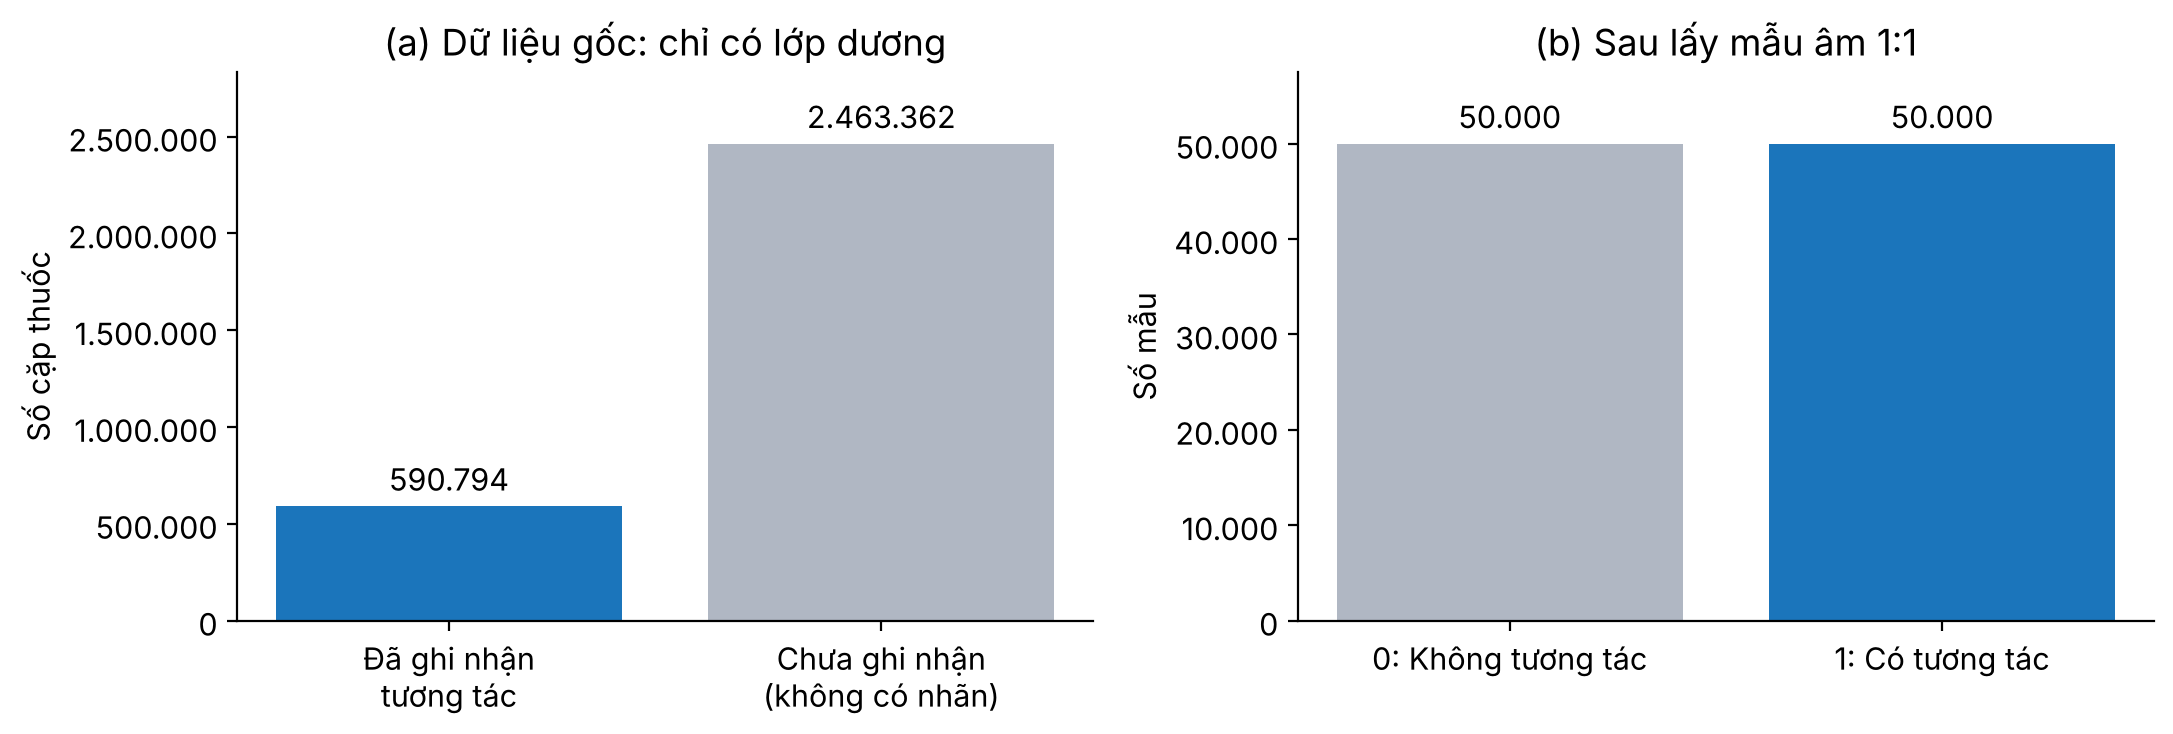
\includegraphics[width=\textwidth]{fig02_phan_bo_nhan.png}
  \caption{Phân bố nhãn: (a) dữ liệu gốc, (b) sau khi lấy mẫu âm}
  \label{fig:phanbonhan}
\end{figure}

\textit{Nhận xét:} Hình~\ref{fig:phanbonhan}a cho thấy DrugBank chỉ ghi nhận
lớp dương: 590.794 cặp có tương tác (19,34\% trong 3.054.156 cặp có thể
ghép từ 2.472 thuốc), 80,66\% cặp còn lại không có nhãn -- không có cặp nào
được xác nhận ``không tương tác''. Do đó phải tạo mẫu âm (Mục~\ref{sec:chatluong}).
Sau khi lấy 50.000 cặp dương và 50.000 cặp âm (Hình~\ref{fig:phanbonhan}b), hai
lớp cân bằng tuyệt đối, nên không cần kỹ thuật cân bằng lớp ở bước huấn luyện.

\begin{figure}[H]
  \centering
  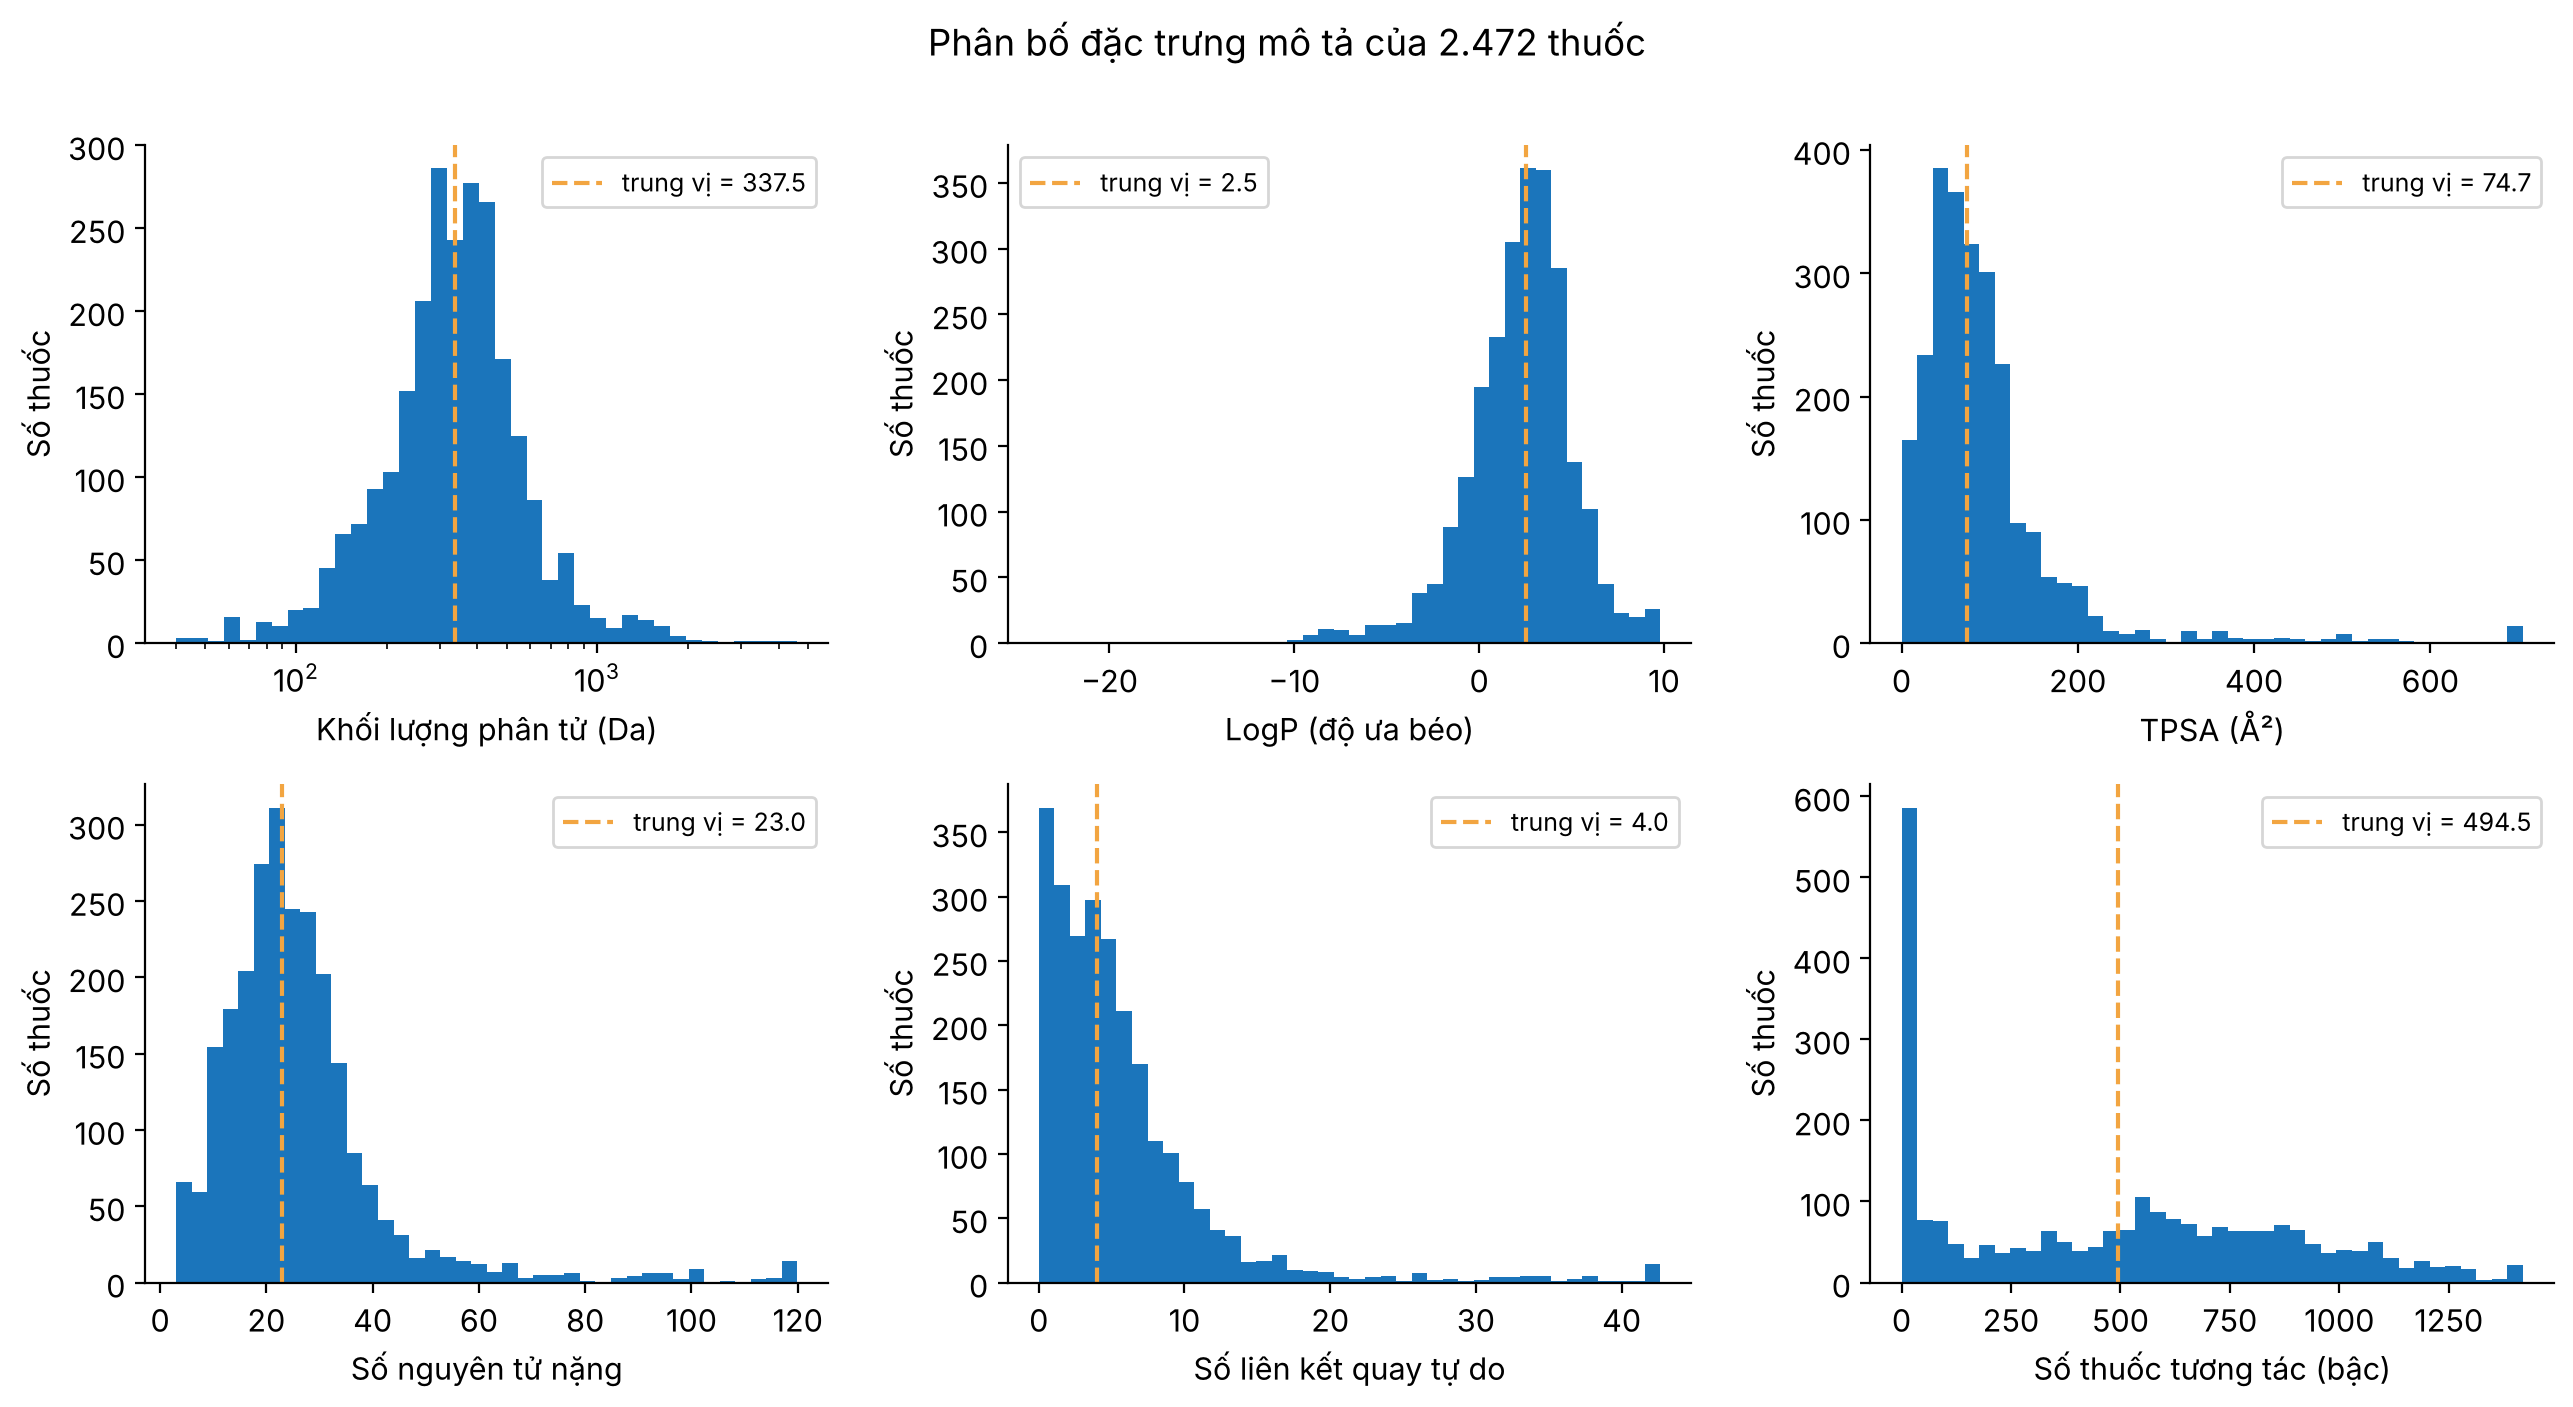
\includegraphics[width=\textwidth]{fig03_phan_bo_mo_ta.png}
  \caption{Phân bố các đặc trưng mô tả chính của thuốc}
  \label{fig:phanbomota}
\end{figure}

\textit{Nhận xét:} Theo Hình~\ref{fig:phanbomota}:
\begin{itemize}
  \item Khối lượng phân tử lệch phải mạnh (độ lệch 5,48): đa số thuốc
        nằm trong khoảng 248--446 Da (trung vị 337 Da, phù hợp quy tắc
        ``thuốc giống thuốc'' $<500$ Da), nhưng có đuôi dài gồm các peptide lớn
        như Imetelstat (4.610 Da), Semaglutide (4.114 Da).
  \item LogP tập trung quanh 2,5 (thuốc ưa béo vừa phải), có một số giá
        trị âm rất lớn ở các phân tử nhiều nhóm phân cực.
  \item TPSA, số nguyên tử nặng, số liên kết quay đều lệch phải và có
        đuôi dài cùng nhóm phân tử lớn; trung vị lần lượt 74,7 Å$^2$, 23 nguyên tử
        và 4 liên kết.
  \item Bậc tương tác phân bố hai đỉnh: 414 thuốc (16,7\%) có bậc 0
        (không tương tác với thuốc nào trong phạm vi), phần còn lại trải rộng
        tới 1.619. Đây là dấu hiệu quan trọng cho việc tạo mẫu âm (Mục~\ref{sec:chatluong}).
\end{itemize}

\begin{figure}[H]
  \centering
  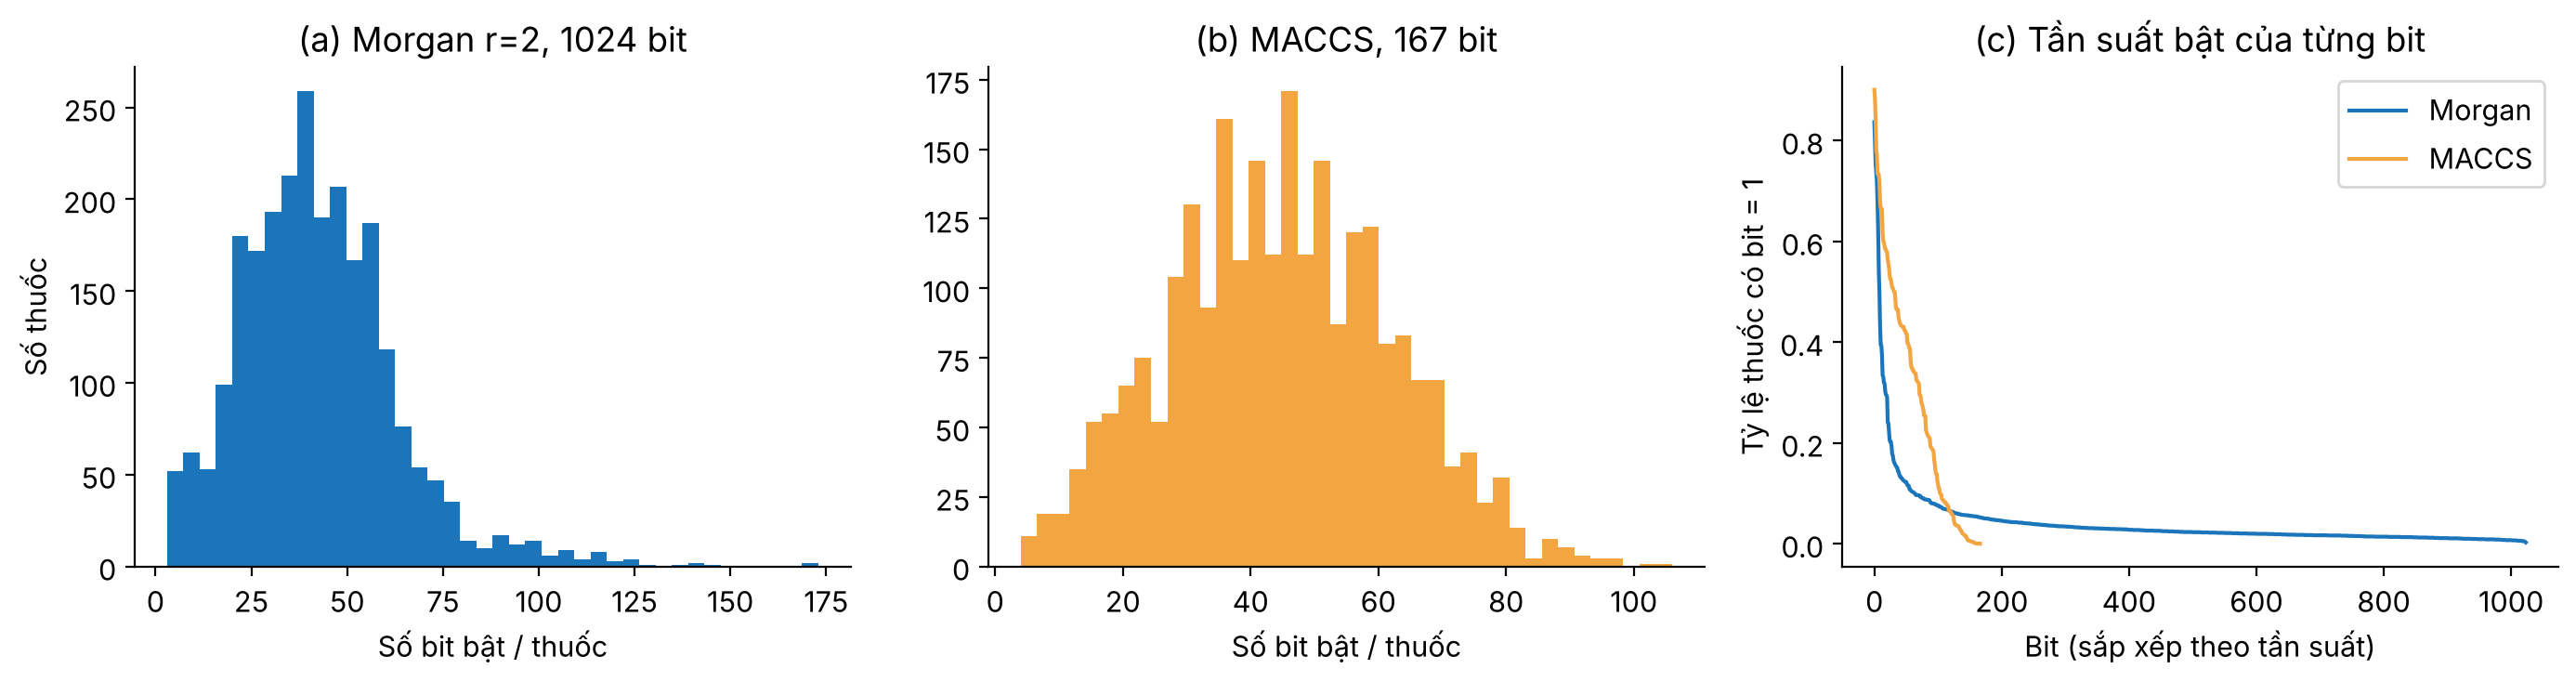
\includegraphics[width=\textwidth]{fig04_fingerprint.png}
  \caption{Đặc trưng vân tay phân tử: số bit bật mỗi thuốc và tần suất bật của từng bit}
  \label{fig:fingerprint}
\end{figure}

\textit{Nhận xét:} Hình~\ref{fig:fingerprint} cho thấy vân tay Morgan rất
thưa: trung vị 40/1.024 bit bằng 1 mỗi thuốc, mật độ trung bình 4,15\%,
đa số bit chỉ bật ở dưới 5\% số thuốc. MACCS dày hơn (trung vị 44/167 bit, mật
độ 26,78\%), một số khóa bật ở trên 80\% thuốc (vd. có vòng), trong khi 6 khóa
không bao giờ bật. Đặc trưng thưa, nhị phân phù hợp với mô hình cây và mô hình
tuyến tính có điều chuẩn.

\subsection{Quan hệ giữa các đặc trưng}
\label{sec:quanhe}

\begin{figure}[H]
  \centering
  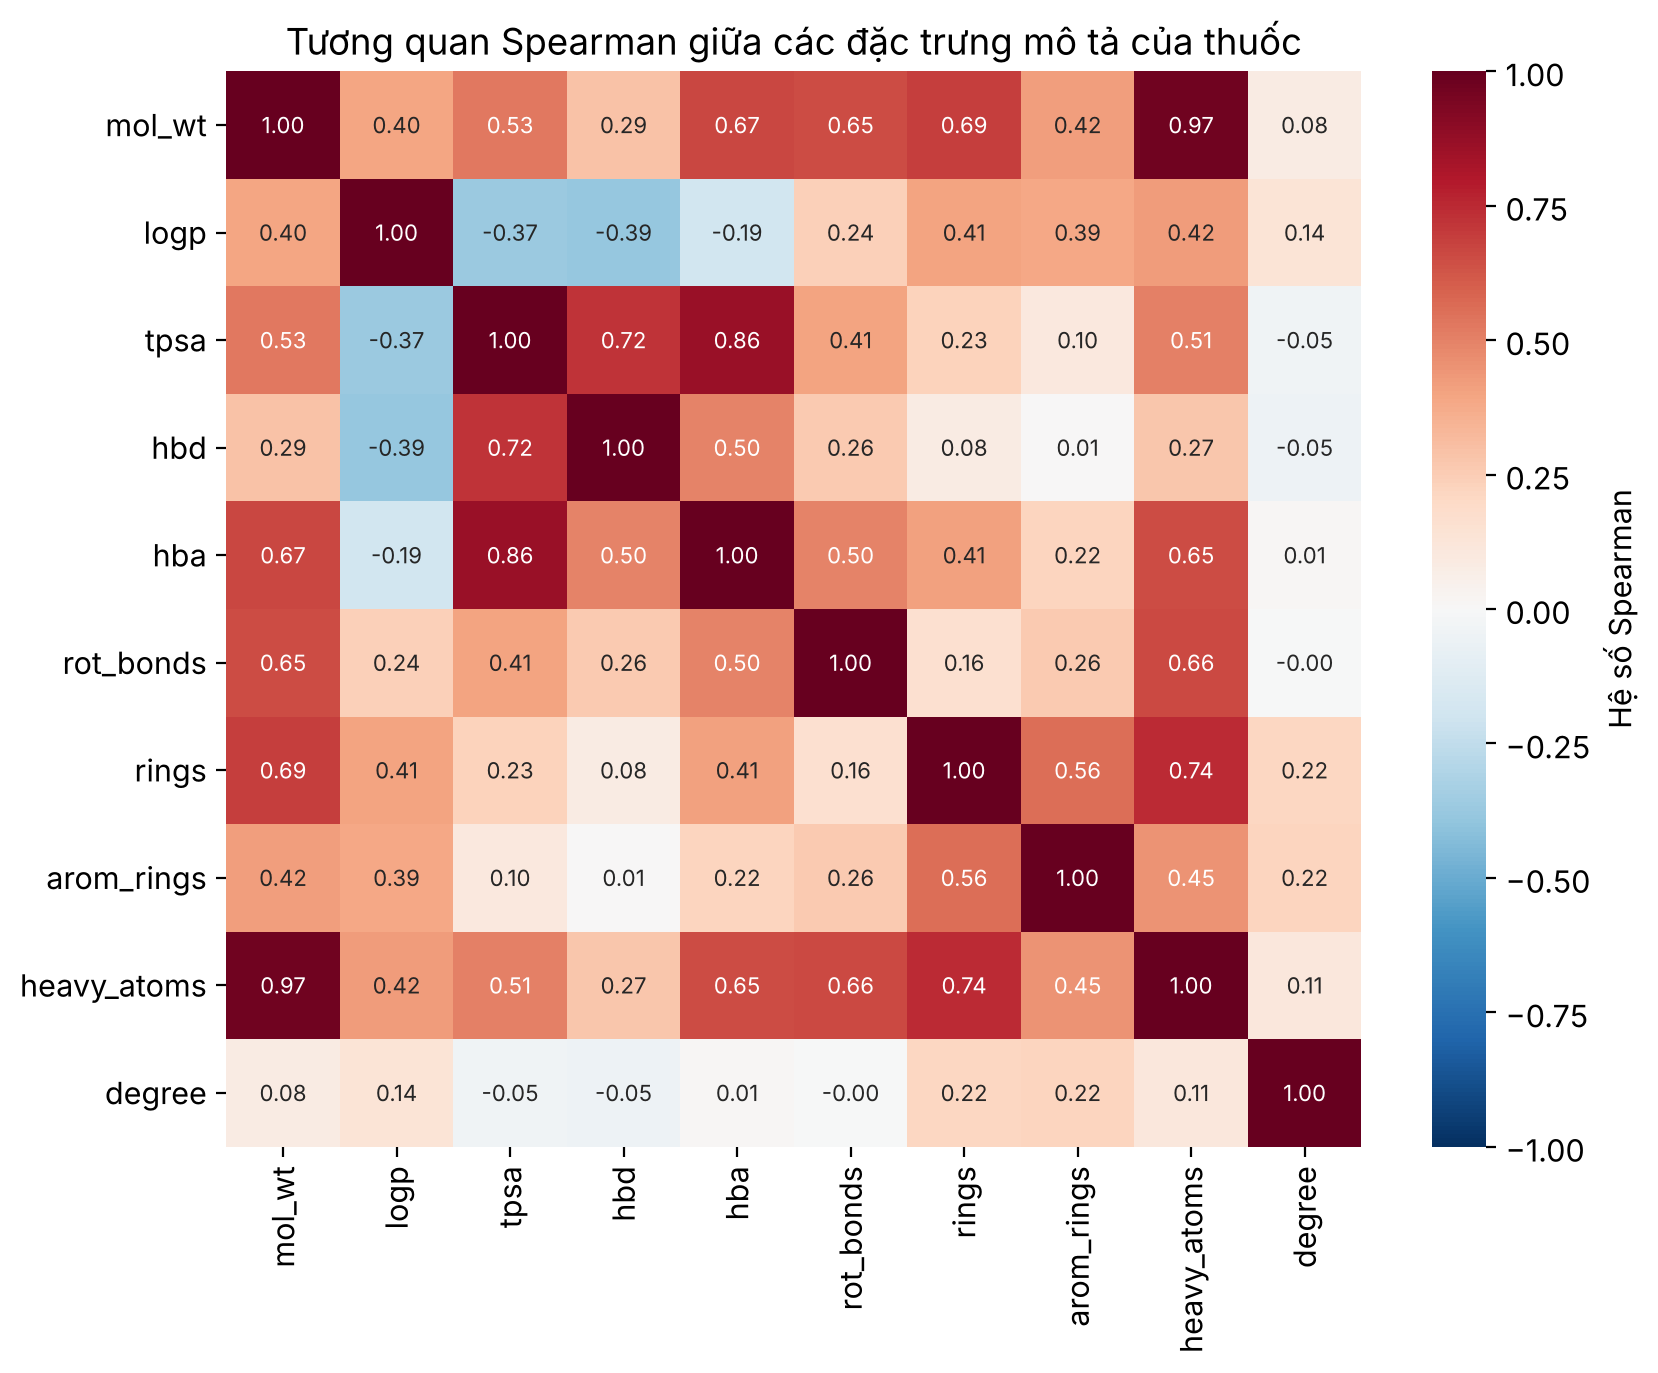
\includegraphics[width=0.78\textwidth]{fig05_tuong_quan.png}
  \caption{Ma trận tương quan Spearman giữa các đặc trưng mô tả của thuốc}
  \label{fig:tuongquan}
\end{figure}

\begin{figure}[H]
  \centering
  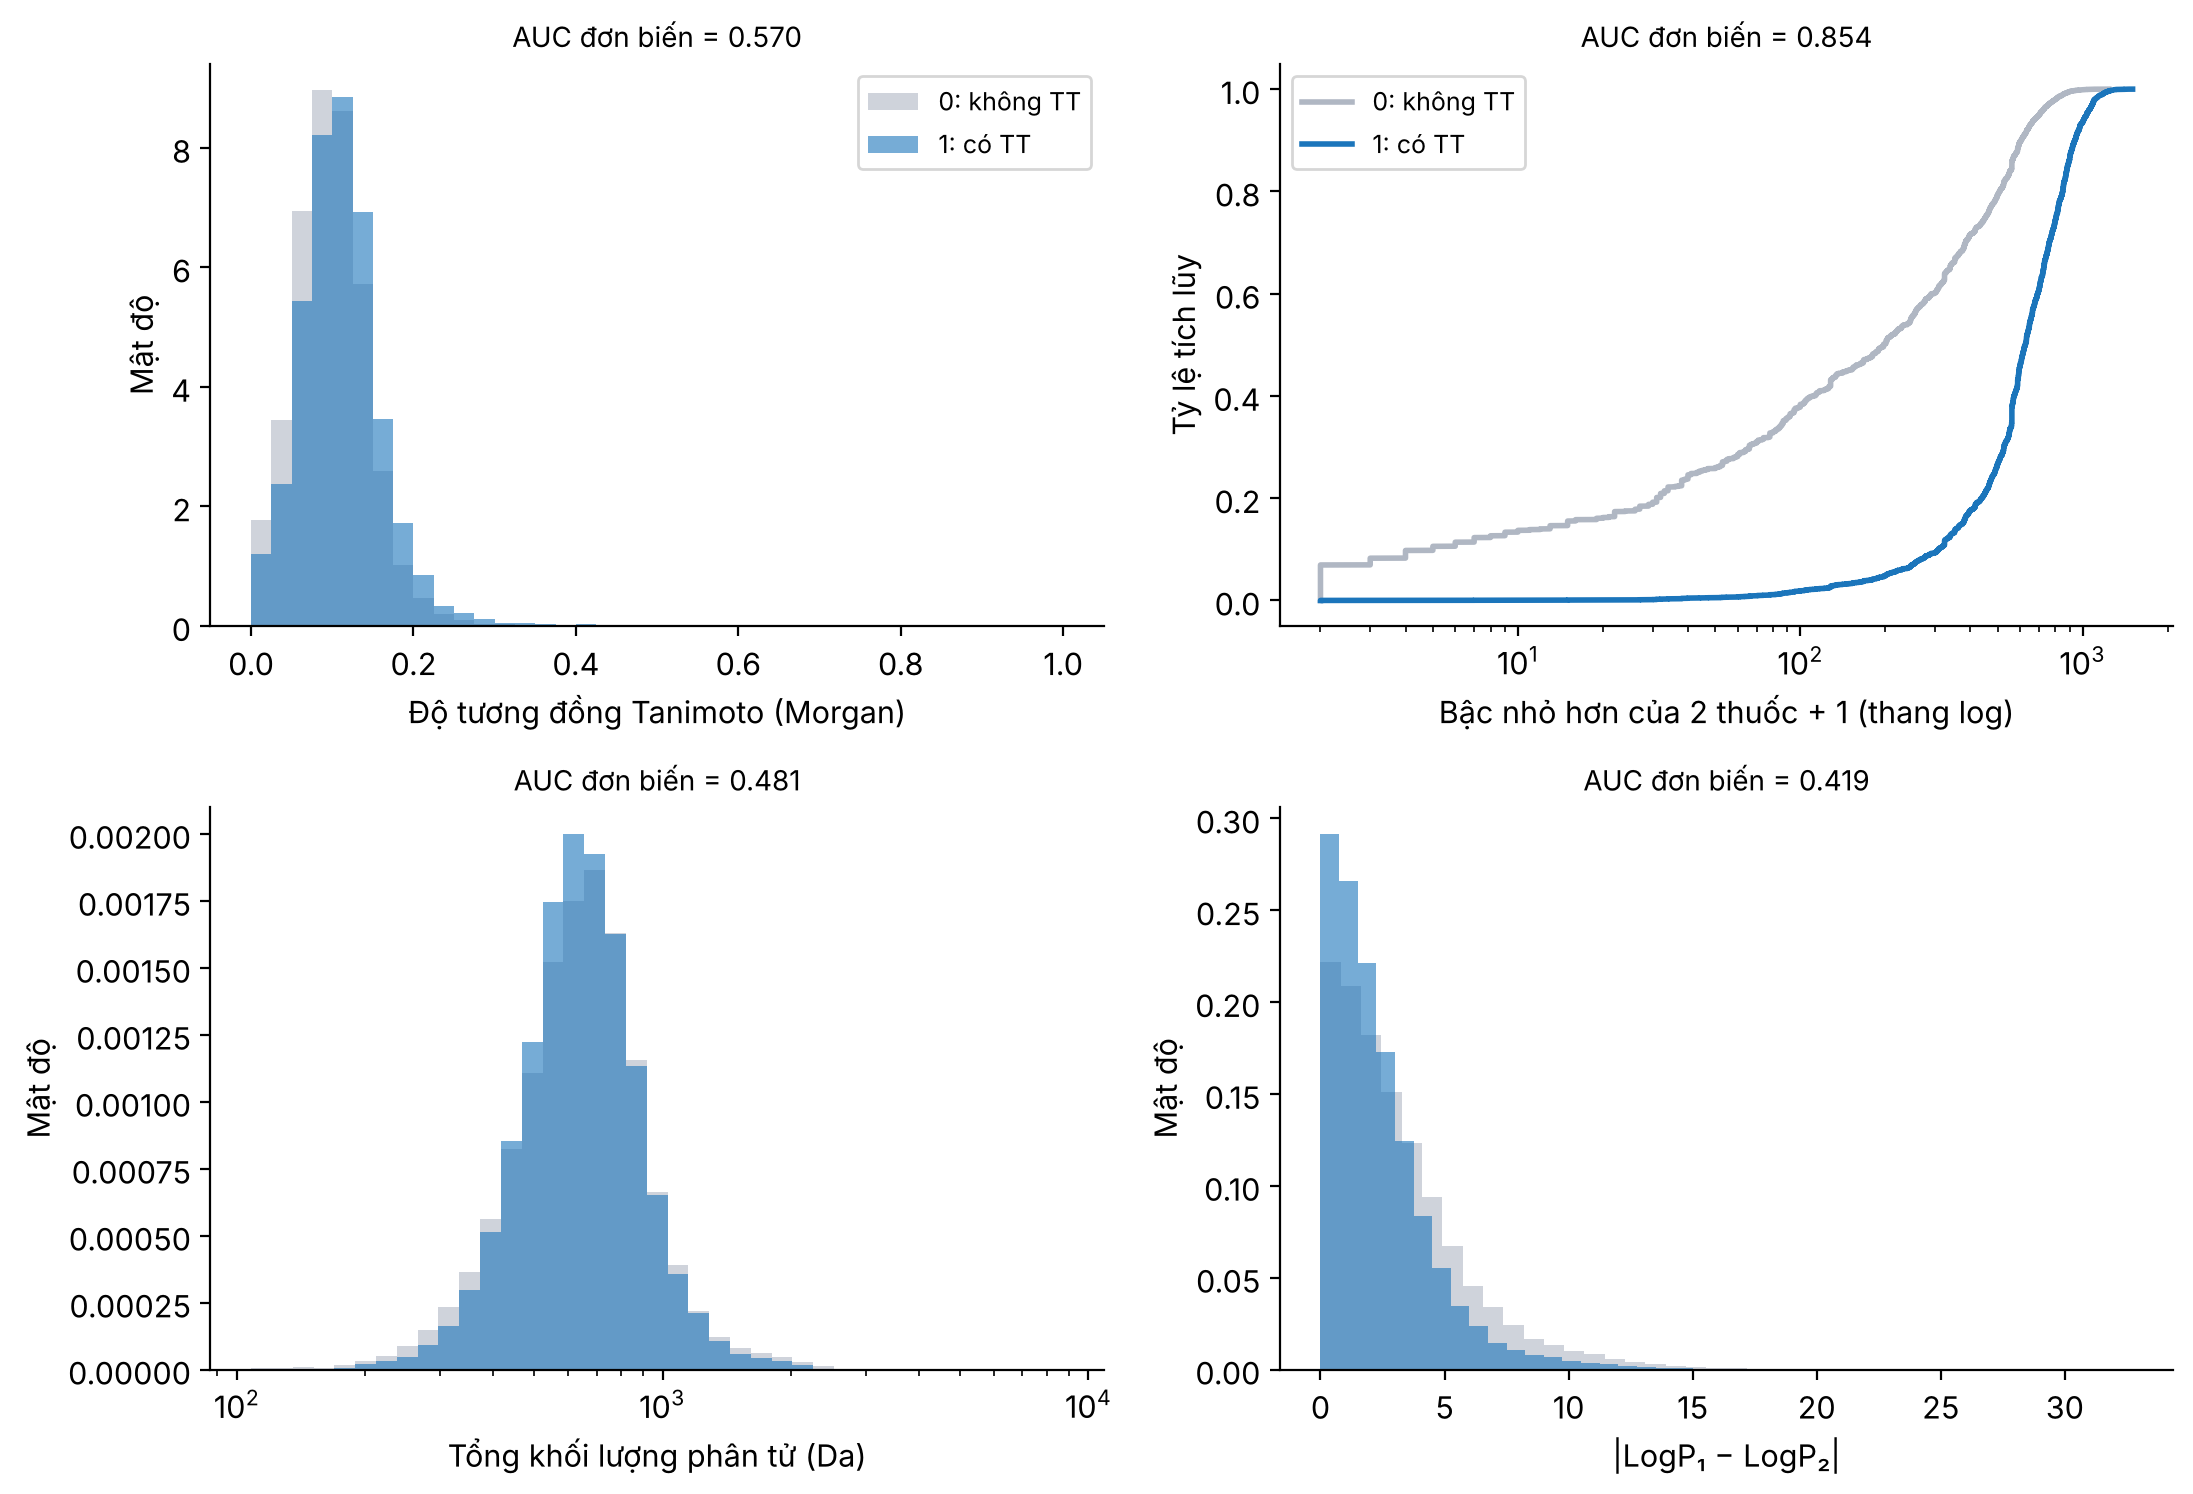
\includegraphics[width=0.92\textwidth]{fig06_dac_trung_cap_theo_nhan.png}
  \caption{Phân bố đặc trưng ở mức cặp thuốc theo nhãn (kèm AUC đơn biến)}
  \label{fig:capnhan}
\end{figure}

\begin{table}[H]
  \centering
  \caption{Đặc trưng ở mức cặp thuốc theo nhãn và AUC khi dùng riêng từng đặc trưng}
  \label{tab:donbien}
  \small
  \begin{tabular}{lccc}
    \toprule
    \textbf{Đặc trưng cặp} & \textbf{TB lớp 1} & \textbf{TB lớp 0} & \textbf{AUC đơn biến} \\
    \midrule
    Độ tương đồng Tanimoto (Morgan) & 0,111 & 0,099 & 0,570 \\
    Bậc nhỏ hơn của hai thuốc & 631,1 & 260,6 & 0,854 \\
    Tổng bậc hai thuốc & 1.613,0 & 965,6 & 0,858 \\
    Tổng khối lượng phân tử (Da) & 761,6 & 801,7 & 0,481 \\
    $|\text{LogP}_A-\text{LogP}_B|$ & 2,42 & 3,16 & 0,419 \\
    Tổng TPSA (Å$^2$) & 172,8 & 201,3 & 0,436 \\
    \bottomrule
  \end{tabular}
\end{table}

\begin{figure}[H]
  \centering
  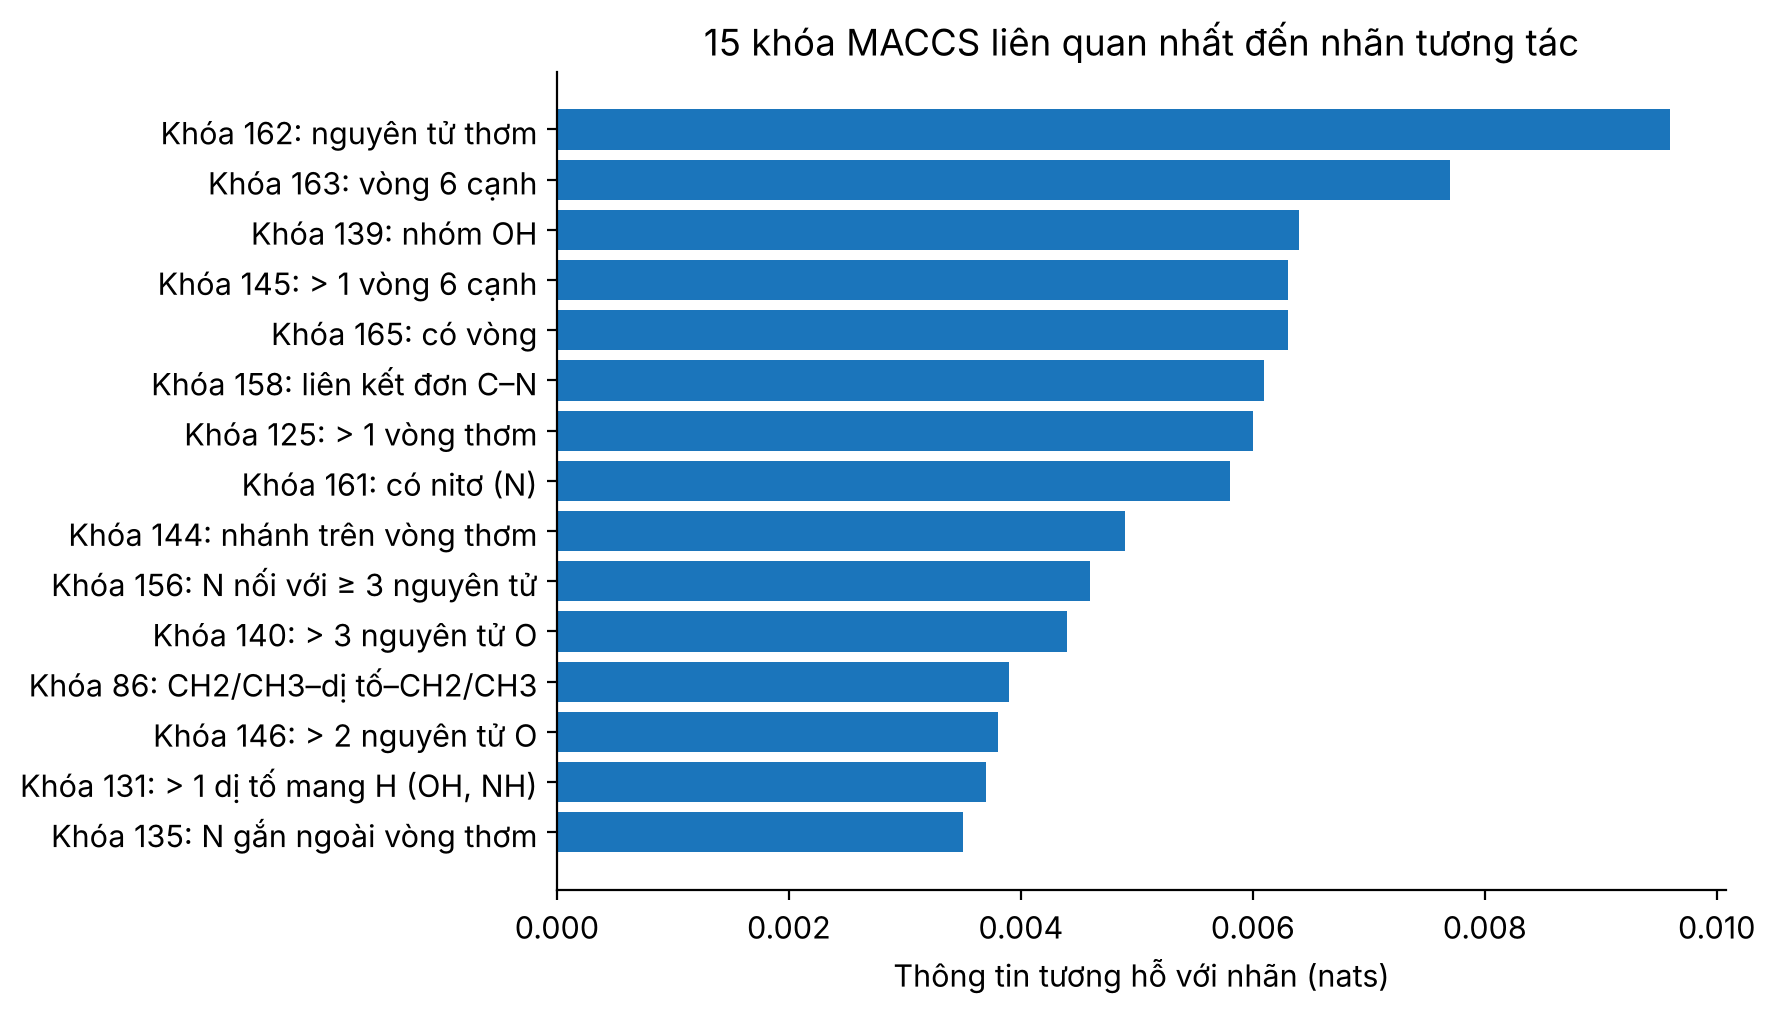
\includegraphics[width=0.85\textwidth]{fig07_maccs_mi.png}
  \caption{15 khóa MACCS có thông tin tương hỗ lớn nhất với nhãn}
  \label{fig:maccsmi}
\end{figure}

\textit{Nhận xét} (Hình~\ref{fig:tuongquan}--\ref{fig:maccsmi}, Bảng~\ref{tab:donbien}):
\begin{enumerate}
  \item Đặc trưng mô tả dư thừa: khối lượng phân tử và số nguyên tử nặng
        tương quan gần tuyệt đối ($\rho=0{,}97$), TPSA tương quan mạnh với số nhóm
        nhận liên kết hydro ($\rho=0{,}86$) và cho liên kết hydro ($\rho=0{,}72$).
        Tương tự, có 22 cặp khóa MACCS tương quan $|r|>0{,}9$. Thông tin cấu trúc
        bị lặp lại nhiều, nên mô hình tuyến tính cần điều chuẩn và có thể cân
        nhắc lựa chọn đặc trưng ở giai đoạn cải tiến.
  \item Mỗi bit cấu trúc riêng lẻ chỉ liên quan yếu đến nhãn: khóa MACCS
        mạnh nhất (khóa 162 -- có nguyên tử thơm) chỉ có MI = 0,0096 nats; các cặp
        tương tác có nhiều vòng thơm hơn (khóa 125 ``>1 vòng thơm'': 78,6\% so
        với 72,9\%) và ít nhóm OH, ít nguyên tử O hơn (khóa 139: 70,3\% so với
        79,4\%). Độ tương đồng Tanimoto giữa hai thuốc cũng chỉ đạt AUC 0,570.
        Vì vậy cần mô hình đa biến, phi tuyến (Random Forest, XGBoost) để kết hợp
        nhiều bit, thay vì dựa vào một vài đặc trưng.
  \item Bậc tương tác của thuốc dự đoán nhãn rất mạnh (AUC đơn biến 0,854
        với bậc nhỏ hơn): các thuốc ``phổ biến'' tham gia nhiều cặp dương, trong
        khi mẫu âm ngẫu nhiên hay chứa thuốc ít tương tác. Bậc được tính từ chính
        nhãn nên không được dùng làm đặc trưng (rò rỉ nhãn); tuy nhiên mô
        hình vẫn có thể gián tiếp học ``độ phổ biến'' của thuốc qua vân tay. Đây là
        thiên lệch cần kiểm soát khi tạo mẫu âm và khi đánh giá theo nhóm thuốc.
  \item Đặc trưng kích thước phân tử gần như không phân biệt nhãn (tổng
        khối lượng phân tử AUC 0,481), nên ngoại lai về kích thước không phải là
        nguồn tín hiệu chính; giữ lại các phân tử lớn không làm lệch mô hình.
  \item Bậc gần như độc lập với đặc trưng mô tả ($|\rho|\leq0{,}22$): độ
        phổ biến của thuốc không giải thích được bằng kích thước hay độ phân cực,
        nghĩa là tín hiệu ``bậc'' và tín hiệu cấu trúc là hai nguồn khác nhau.
\end{enumerate}

\section{Chất lượng dữ liệu và xây dựng tập mẫu âm}
\label{sec:chatluong}

\subsection{Phát hiện và xử lý vấn đề chất lượng dữ liệu}
Các vấn đề chất lượng dữ liệu được định lượng và xử lý như trong
Bảng~\ref{tab:chatluong}; so sánh trước -- sau xử lý ở Hình~\ref{fig:truocsau}.

{\small
\begin{xltabular}{\textwidth}{p{3.4cm} >{\centering\arraybackslash}p{2.6cm} X}
\caption{Thống kê các vấn đề chất lượng dữ liệu và cách xử lý}\label{tab:chatluong}\\
\toprule
\textbf{Vấn đề} & \textbf{Số lượng (tỷ lệ)} & \textbf{Cách xử lý và lý do} \\ \midrule
\endfirsthead
\multicolumn{3}{l}{\textit{Bảng \thetable\ (tiếp theo)}}\\ \toprule
\textbf{Vấn đề} & \textbf{Số lượng (tỷ lệ)} & \textbf{Cách xử lý và lý do} \\ \midrule
\endhead
\bottomrule
\endlastfoot
    Bản ghi tương tác trùng (A--B và B--A) & 1.427.655 / 2.855.848 (49,99\%) & Gộp thành cặp không thứ tự (A < B). Nếu giữ cả hai chiều, cùng một tương tác có thể rơi vào cả tập train và test, gây rò rỉ. \\
    Cặp tham chiếu thuốc không có trong bảng thuốc & 538 / 1.428.193 (0,04\%) & Loại bỏ vì không có thông tin cấu trúc. \\
    Thiếu SMILES & 5.117 / 17.430 (29,36\%); trong phạm vi: 157 / 2.802 (5,60\%) & Chủ yếu là thuốc sinh học (4.264). Giới hạn phạm vi vào thuốc phân tử nhỏ đã phê duyệt, loại 157 thuốc thiếu SMILES: không thể điền khuyết cấu trúc hóa học. \\
    SMILES không hợp lệ & 2 / 2.802 (0,07\%) & Loại bỏ (RDKit không đọc được). \\
    SMILES nhiều thành phần (muối, nước kết tinh) & 246 / 2.802 (8,78\%) & Giữ thành phần lớn nhất (\texttt{LargestFragmentChooser}): ion đối như Na$^+$, Cl$^-$ không quyết định hoạt tính nhưng làm vân tay khác nhau giữa các dạng muối. \\
    Thành phần chính quá nhỏ ($\leq2$ nguyên tử nặng) & 84 / 2.802 (3,00\%) & Loại bỏ (ion, chất vô cơ như K, Fe, NaCl): vân tay gần như toàn 0, không mang thông tin cấu trúc. \\
    Trùng cấu trúc (khác mã, cùng phân tử) & 87 mã thừa (3,10\%), 129 mã thuộc 42 cấu trúc & Gộp về một mã đại diện (mã có nhiều tương tác nhất), ánh xạ cặp tương tác sang mã đại diện. Nếu không, các mẫu có đặc trưng giống hệt nhau xuất hiện ở cả train và test. \\
    Ngoại lai kích thước phân tử (IQR) & \texttt{mol\_wt}: 154 (6,2\%); \texttt{tpsa}: 135 (5,5\%) & Giữ lại: đây là thuốc thật (peptide, kháng sinh lớn); vân tay là đặc trưng nhị phân nên không bị ảnh hưởng bởi độ lớn giá trị; kích thước gần như không liên quan đến nhãn (Bảng~\ref{tab:donbien}). \\
    Mất cân bằng lớp & 100\% dương; 0 cặp âm được ghi nhận & Lấy mẫu âm 1:1 từ các cặp chưa ghi nhận tương tác (loại mọi cặp có trong DrugBank). \\
    Thiên lệch khi lấy mẫu âm & 414 thuốc bậc 0; 37,9\% mẫu âm chứa thuốc bậc 0 & Chỉ ghép mẫu âm trong 2.058 thuốc có $\geq1$ tương tác (như Ran \textit{et al.}): tỷ lệ còn 0\%, AUC của ``bậc'' giảm từ 0,909 xuống 0,854 (Bảng~\ref{tab:mauam}). \\
    Nguy cơ rò rỉ khi chia theo cặp & 100\% thuốc của tập kiểm tra có mặt trong tập huấn luyện & Bổ sung đánh giá chia theo nhóm thuốc (Mục~\ref{sec:chuanbi}); không dùng mã thuốc, bậc làm đặc trưng. \\
\end{xltabular}
}

\begin{figure}[H]
  \centering
  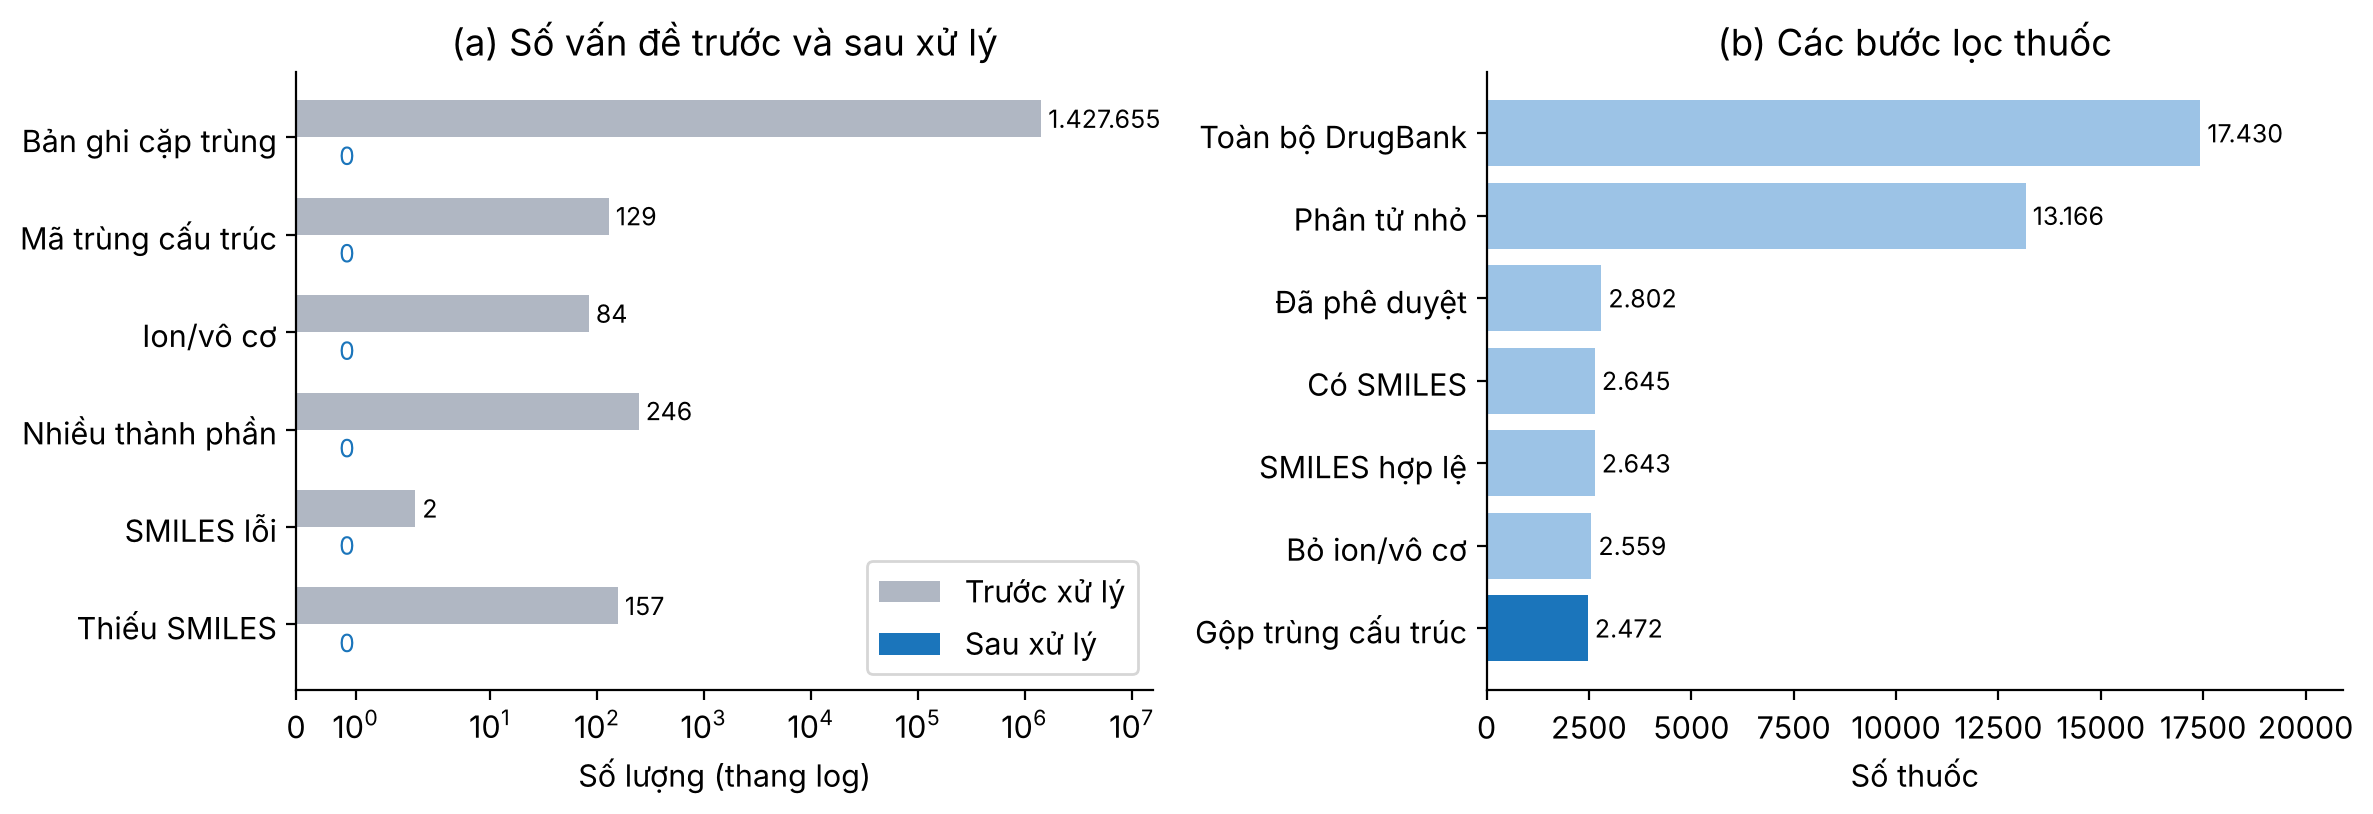
\includegraphics[width=\textwidth]{fig01_truoc_sau_lam_sach.png}
  \caption{So sánh trước -- sau xử lý: (a) số vấn đề, (b) số thuốc qua từng bước lọc}
  \label{fig:truocsau}
\end{figure}

\textit{Nhận xét:} Hình~\ref{fig:truocsau}a cho thấy toàn bộ các vấn đề đã phát
hiện đều được đưa về 0 sau xử lý. Hình~\ref{fig:truocsau}b thể hiện số thuốc
giảm từ 17.430 xuống 2.472 qua các bước lọc; bước giảm lớn nhất là giới hạn vào
thuốc đã phê duyệt (13.166 $\rightarrow$ 2.802). Việc ánh xạ mã trùng cấu trúc
làm giảm thêm 11.469 cặp tương tác trùng lặp, còn 590.794 cặp dương.

\subsection{Xây dựng tập mẫu âm}
\label{sec:mauam}

Vì DrugBank chỉ ghi nhận các cặp có tương tác (Mục~\ref{sec:ddi}), bài toán
rơi vào tình huống học từ dữ liệu dương và chưa gán nhãn
(Mục~\ref{sec:ddihocmay}). Nhóm so sánh hai phương án lấy mẫu âm và chọn phương
án giảm thiên lệch theo bậc (Bảng~\ref{tab:mauam}).

\begin{table}[H]
  \centering
  \caption{So sánh hai phương án lấy mẫu âm (cùng 50.000 cặp dương)}
  \label{tab:mauam}
  \small
  \begin{tabularx}{\textwidth}{X >{\centering\arraybackslash}p{2.4cm} >{\centering\arraybackslash}p{2.8cm} >{\centering\arraybackslash}p{2.8cm}}
    \toprule
    \textbf{Phương án} & \textbf{Số thuốc dùng để ghép} & \textbf{\% mẫu âm chứa thuốc bậc 0} & \textbf{AUC đơn biến của ``bậc nhỏ hơn''} \\
    \midrule
    1: Ghép ngẫu nhiên trong toàn bộ 2.472 thuốc & 2.472 & 37,9\% & 0,909 \\
    2 (chọn): Chỉ ghép trong thuốc có $\geq 1$ tương tác & 2.058 & 0,0\% & 0,854 \\
    \bottomrule
  \end{tabularx}
\end{table}

\textit{Nhận xét:} Với phương án 1, gần 38\% mẫu âm chứa một thuốc chưa từng
tương tác, mô hình có thể đạt điểm cao chỉ nhờ nhận ra ``thuốc lạ'' thay vì học
quan hệ cấu trúc. Phương án 2 loại bỏ hoàn toàn trường hợp này và giảm sức mạnh
dự đoán của ``bậc'' (AUC 0,909 $\rightarrow$ 0,854). Thiên lệch không mất hẳn
do thuốc phổ biến vẫn xuất hiện nhiều hơn ở lớp dương; nhóm sẽ đánh giá thêm
phương án lấy mẫu âm cân bằng theo bậc ở Mục~\ref{sec:tongquat}.

\section{Biểu diễn đặc trưng cặp thuốc}
\label{sec:bieudiencap}
Đây là bước chuyển từ thuốc sang cặp thuốc -- đơn vị mẫu thực sự
của bài toán -- và là khâu then chốt của quy trình, vì mọi thuật toán phía sau
đều chỉ nhìn thấy kết quả của bước này.

\subsection{Vectơ đặc trưng của một thuốc}
Mỗi thuốc $A$ sau khi chuẩn hóa SMILES được mã hóa thành vectơ
\begin{equation}
  \phi(A) = \big[\, \mathrm{Morgan}(A) \,\|\, \mathrm{MACCS}(A) \,\big]
  \in \{0,1\}^{1.191},
  \label{eq:phi}
\end{equation}
gồm vân tay Morgan bán kính 2 với 1.024 bit~\eqref{eq:bang} và 167 khóa MACCS,
tính bằng RDKit \cite{rdkit}. Hai loại vân tay được ghép vì chúng bổ sung cho
nhau (Mục~\ref{sec:vantay}): Morgan cho độ phân giải cao, MACCS cho các nhóm
chức đã được chuyên gia chọn lọc. Ngoài ra mỗi thuốc còn có vectơ 9 đặc trưng
hóa lý $\psi(A) \in \mathbb{R}^{9}$ (Bảng~\ref{tab:hoaly}), chỉ dùng ở phương án
biểu diễn mở rộng.

\subsection{Ba phương án ghép cặp}
Theo phân tích ở Mục~\ref{sec:ddihocmay}, nhóm triển khai và so sánh ba phương
án (Bảng~\ref{tab:bieudien}).

(1) Ghép nối (\texttt{concat}). Vectơ cặp là
\begin{equation}
  \mathbf{x}_{\text{concat}}(A,B) = \big[\, \phi(A) \,\|\, \phi(B) \,\big]
  \in \{0,1\}^{2.382},
  \label{eq:concat}
\end{equation}
với quy ước thuốc có mã DrugBank nhỏ hơn đứng trước. Đây là phương án dùng ở
giai đoạn đầu, giữ được toàn bộ thông tin của hai thuốc nhưng không thỏa
mãn điều kiện đối xứng~\eqref{eq:doixung}: cùng một cặp thuốc cho hai vectơ khác
nhau tùy thứ tự. Quy ước sắp theo mã thuốc còn kéo theo một hệ quả tinh vi --
mã DrugBank phản ánh thời điểm thuốc được đưa vào cơ sở dữ liệu, nên vị trí
trong vectơ vô tình mang một phần thông tin về ``tuổi'' và độ phổ biến của
thuốc. Mục~\ref{sec:hanche2} định lượng ảnh hưởng này.

(2) Đối xứng bằng phép cộng (\texttt{sum}).
\begin{equation}
  \mathbf{x}_{\text{sum}}(A,B) = \phi(A) + \phi(B) \in \{0,1,2\}^{1.191} .
  \label{eq:sum}
\end{equation}
Phương án này thỏa mãn~\eqref{eq:doixung} theo thiết kế và giảm một nửa số
chiều. Mỗi thành phần nhận ba giá trị mang ý nghĩa hóa học trực tiếp: 0 -- mảnh
cấu trúc không có ở thuốc nào; 1 -- có ở đúng một trong hai thuốc; 2 --
có ở cả hai. Thông tin bị mất là mảnh đó thuộc thuốc nào khi giá
trị bằng 1. Nhóm chọn phép cộng thay vì tích Hadamard hay hiệu tuyệt đối vì
phép cộng giữ được cả ba trạng thái trên, trong khi tích chỉ giữ lại trường hợp
``cả hai cùng có'' và hiệu tuyệt đối chỉ giữ ``đúng một bên có''.

(3) Đối xứng mở rộng (\texttt{sum\_plus}). Bổ sung hai cải tiến cho
phương án (2): dùng vân tay Morgan dạng đếm thay vì nhị phân (giữ lại số
lần một mảnh cấu trúc xuất hiện), và thêm 9 đặc trưng hóa lý dưới hai dạng toán
tử đối xứng -- tổng và trị tuyệt đối của hiệu:
\begin{equation}
  \mathbf{x}_{\text{sum\_plus}}(A,B) = \Big[\,
  \phi_{\text{đếm}}(A) + \phi_{\text{đếm}}(B)
  \;\big\|\; \psi(A) + \psi(B)
  \;\big\|\; \big|\psi(A) - \psi(B)\big| \,\Big]
  \in \mathbb{R}^{1.209} .
  \label{eq:sumplus}
\end{equation}
Hai dạng toán tử này mang thông tin khác nhau: tổng mô tả ``tải'' chung
của cặp (vd. tổng khối lượng phân tử, tổng độ ưa béo), còn hiệu tuyệt đối
mô tả mức chênh lệch giữa hai thuốc. Cơ sở để thêm nhóm đặc trưng này là
phân tích cơ chế ở Mục~\ref{sec:ddi}: tương tác dược động học phụ thuộc vào độ
ưa béo, kích thước và số nhóm chức -- những đại lượng mà vân tay nhị phân không
mã hóa trực tiếp.

\begin{table}[H]
  \centering
  \caption{Ba phương án biểu diễn cặp thuốc}
  \label{tab:bieudien}
  \small
  \begin{tabularx}{\textwidth}{>{\raggedright\arraybackslash}p{2.6cm}
      >{\centering\arraybackslash}p{1.6cm} >{\centering\arraybackslash}p{1.9cm} X}
    \toprule
    \textbf{Phương án} & \textbf{Số chiều} & \textbf{Đối xứng} & \textbf{Thông tin được giữ / bị mất} \\
    \midrule
    \texttt{concat}~\eqref{eq:concat} & 2.382 & Không & Giữ toàn bộ, kể cả thông tin mảnh thuộc thuốc nào; phụ thuộc quy ước thứ tự \\
    \texttt{sum}~\eqref{eq:sum} & 1.191 & Có & Giữ ``có ở một hay cả hai''; mất thông tin mảnh thuộc thuốc nào \\
    \texttt{sum\_plus}~\eqref{eq:sumplus} & 1.209 & Có & Như trên, thêm số lần xuất hiện của mảnh và đặc trưng hóa lý (tổng, $|$hiệu$|$) \\
    \bottomrule
  \end{tabularx}
\end{table}

Ngoài ba phương án trên, nhóm còn thử đối xứng hóa ở bước dự đoán: huấn
luyện trên \texttt{concat} nhưng khi dự đoán thì lấy trung bình xác suất của
$(A,B)$ và $(B,A)$. Kết quả của cả bốn phương án được so sánh ở
Mục~\ref{sec:caitien}.

\subsection{Cài đặt}
Toàn bộ bước này nằm trong mô-đun \texttt{src/ddi\_features.py} để hai notebook
huấn luyện dùng chung, bảo đảm mọi mô hình nhìn thấy đúng cùng một cách biểu
diễn. Ma trận đặc trưng được giữ ở kiểu
\texttt{uint8} thay vì \texttt{float64}: với 100.000 mẫu $\times$ 2.382 chiều,
cách này giảm bộ nhớ từ khoảng 1,9~GB xuống 238~MB -- yếu tố quyết định để chạy
được trên máy RAM 8~GB. Việc ép kiểu sang \texttt{float32} chỉ thực hiện bên
trong \texttt{Pipeline} cho các mô hình cần (hồi quy Logistic, SVM).

\section{Chia tập và chuẩn bị dữ liệu}
\label{sec:chuanbi}
\begin{itemize}
  \item Mã hóa: không có biến phân loại nào đưa vào mô hình; cấu trúc
        hóa học (SMILES) được mã hóa thành vân tay nhị phân Morgan (bán kính 2,
        1.024 bit) và MACCS (167 bit) bằng RDKit; vectơ cặp ghép nối hai thuốc
        theo thứ tự mã (2.382 chiều, kiểu \texttt{uint8}).
  \item Chia tập: hold-out phân tầng theo nhãn 80/20 với
        \texttt{random\_state = 42} (Bảng~\ref{tab:kichthuoc}); tập kiểm tra giữ
        nguyên đến đánh giá cuối. Ngoài ra, chia theo nhóm thuốc: chọn ngẫu nhiên
        20\% thuốc làm ``thuốc mới'', cặp có 1 hoặc 2 thuốc mới tạo thành tập
        S1, S2.
  \item Lọc đặc trưng và chuẩn hóa: \texttt{VarianceThreshold} và
        \texttt{StandardScaler} chỉ được \texttt{fit} trên tập huấn luyện rồi áp
        dụng cho tập kiểm tra: 16/2.382 bit luôn bằng 0 trên tập huấn luyện bị
        loại; sau chuẩn hóa, tập huấn luyện có trung bình 0, độ lệch chuẩn 1, tập
        kiểm tra có trung bình $\approx 0$, độ lệch chuẩn 1,001. Chuẩn hóa chỉ
        cần cho LR, SVM; khi huấn luyện, các bước này nằm trong \texttt{Pipeline}
        nên được fit lại trên từng fold huấn luyện.
\end{itemize}

\begin{table}[H]
  \centering
  \caption{Kích thước các tập dữ liệu sau khi chia}
  \label{tab:kichthuoc}
  \small
  \begin{tabular}{lccc}
    \toprule
    \textbf{Tập dữ liệu} & \textbf{Số mẫu} & \textbf{Số đặc trưng} & \textbf{Tỷ lệ lớp dương} \\
    \midrule
    Huấn luyện (hold-out) & 80.000 & 2.382 & 0,500 \\
    Kiểm tra (hold-out)   & 20.000 & 2.382 & 0,500 \\
    \midrule
    Theo thuốc: huấn luyện (2 thuốc đã biết) & 63.756 & 2.382 & 0,495 \\
    Theo thuốc: S1 (1 thuốc mới) & 32.208 & 2.382 & 0,508 \\
    Theo thuốc: S2 (2 thuốc mới) & 4.036 & 2.382 & 0,513 \\
    \bottomrule
  \end{tabular}
\end{table}

\begin{figure}[H]
  \centering
  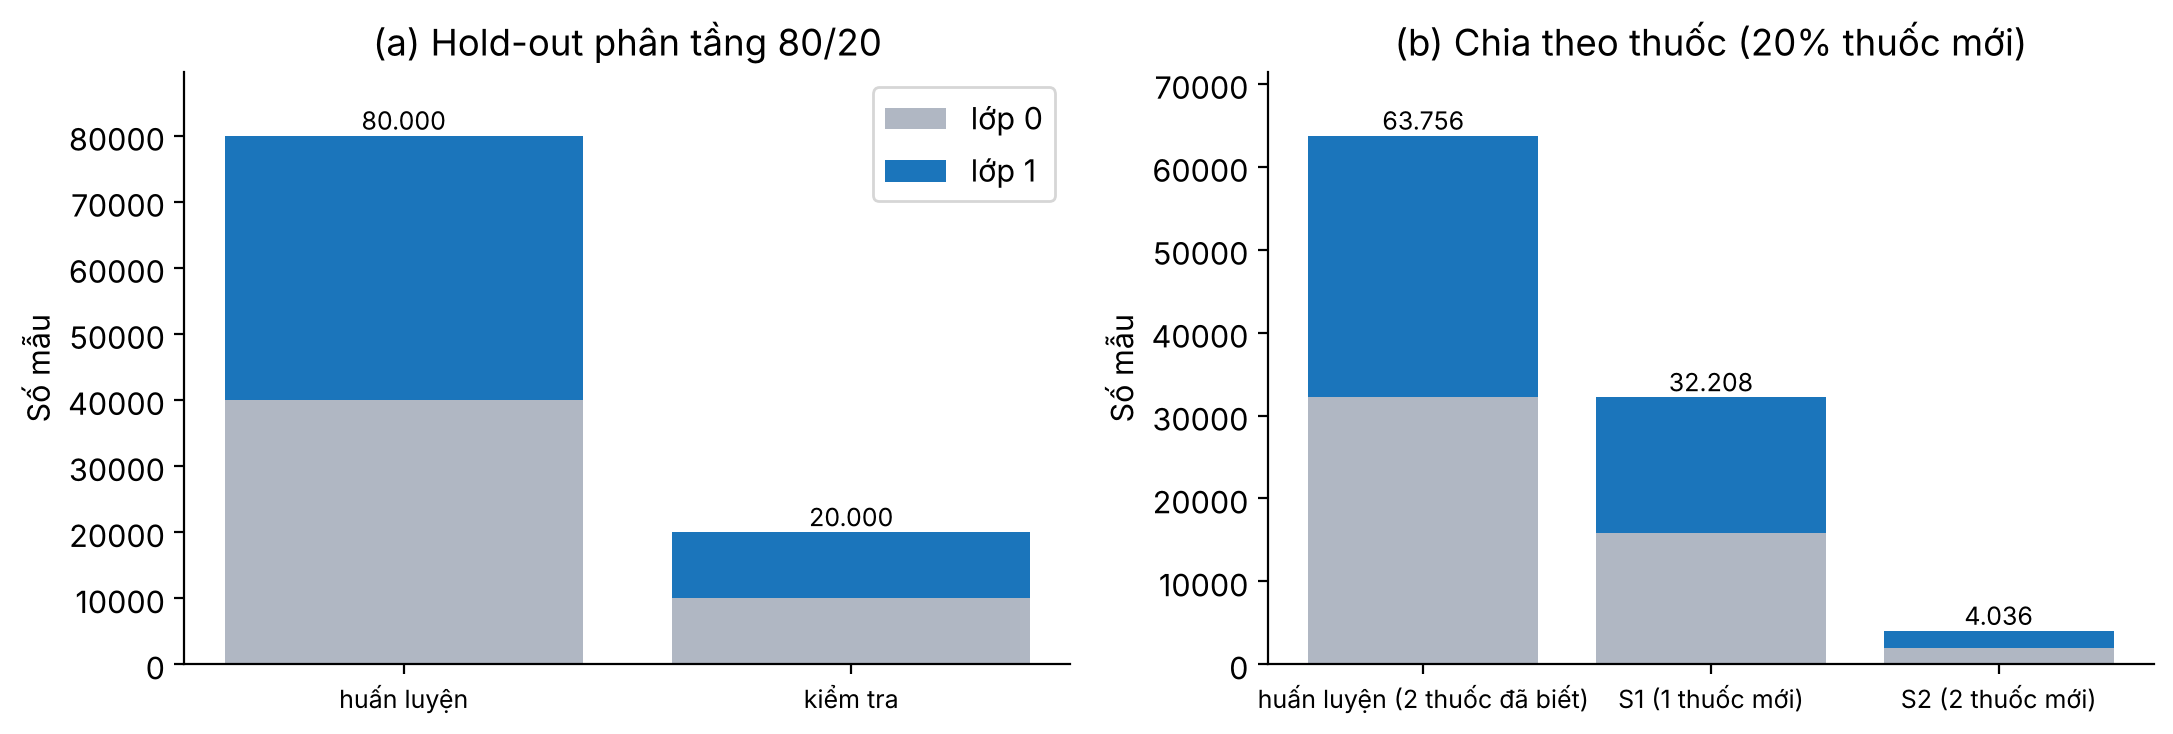
\includegraphics[width=\textwidth]{fig08_chia_tap.png}
  \caption{Kích thước và tỷ lệ lớp của các tập dữ liệu}
  \label{fig:chiatap}
\end{figure}

\textit{Nhận xét:} Hình~\ref{fig:chiatap}a cho thấy hai tập hold-out giữ đúng
tỷ lệ lớp 50/50 nhờ phân tầng. Khi chia theo cặp, toàn bộ thuốc của tập kiểm
tra đều đã xuất hiện trong tập huấn luyện, nên kết quả trên tập này phản ánh
khả năng dự đoán cho thuốc đã biết. Các tập S1, S2 (Hình~\ref{fig:chiatap}b)
vẫn gần cân bằng và đủ lớn (4.036 cặp ở S2) để đo khả năng tổng quát hóa cho
thuốc mới.

\section{Thuật toán, huấn luyện và đánh giá}
\label{sec:quytrinh}
Mục này khép lại quy trình: sau khi đã có ma trận đặc trưng và cách chia tập,
còn phải chọn thuật toán, thiết kế quy trình huấn luyện không rò rỉ dữ liệu và
chốt cách đánh giá. Cơ sở toán học của các thuật toán đã trình bày ở
Mục~\ref{sec:cosotoan}; ở đây chỉ nêu lý do chọn và cách cấu hình.

\subsection{Lựa chọn thuật toán}
Dữ liệu có 80.000 mẫu huấn luyện, 2.382 đặc trưng nhị phân thưa (chỉ khoảng 4\%
bit Morgan bằng 1), hai lớp cân bằng, và tín hiệu nằm ở tổ hợp nhiều bit hơn là ở
từng bit riêng lẻ (Mục~\ref{sec:quanhe}). Từ đặc điểm đó, nhóm chọn bốn thuật toán
(Bảng~\ref{tab:chonthuattoan}).

\begin{table}[H]
  \centering
  \caption{Các thuật toán được chọn và lý do}
  \label{tab:chonthuattoan}
  \small
  \begin{tabularx}{\textwidth}{>{\raggedright\arraybackslash}p{3.1cm} X}
    \toprule
    \textbf{Thuật toán} & \textbf{Lý do lựa chọn với dữ liệu của nhóm} \\
    \midrule
    Logistic Regression & Mô hình tuyến tính, nhanh, diễn giải được qua trọng số; làm mốc để biết bài toán có cần mô hình phi tuyến không. Cần điều chuẩn vì nhiều đặc trưng tương quan. \\
    Random Forest & Phù hợp đặc trưng nhị phân nhiều chiều, tự nắm bắt tương tác giữa các bit, không cần chuẩn hóa; là phương pháp chính của Ran \textit{et al.} \cite{ran2022}. \\
    XGBoost & Boosting trên cây, thường cho độ chính xác cao trên dữ liệu bảng; có điều chuẩn trong hàm mục tiêu, huấn luyện nhanh nhờ thuật toán histogram. \\
    SVM nhân RBF & Biên phi tuyến, mạnh với dữ liệu nhiều chiều; dùng làm đối chứng, chỉ chạy trên một fold vì thời gian huấn luyện tăng xấp xỉ bậc hai theo số mẫu. \\
    \bottomrule
  \end{tabularx}
\end{table}

\subsection{Mô hình cơ sở}
Mô hình cơ sở thứ nhất là \texttt{DummyClassifier} dự đoán xác suất bằng tỷ lệ
lớp (ROC-AUC $=0{,}5$, nhãn theo lớp đa số). Mô hình cơ sở thứ hai là Logistic
Regression với tham số mặc định ($C=1$), làm mốc tuyến tính đơn giản.

\subsection{Quy trình huấn luyện}

Quy trình huấn luyện và đánh giá được mô tả trong Hình~\ref{fig:quytrinhhuanluyen}.
Dữ liệu được chia thành tập huấn luyện và tập kiểm tra ngay từ đầu; các bước lọc
đặc trưng hằng số, chuẩn hóa và mô hình được tổ chức trong \texttt{Pipeline} của
Scikit-learn \cite{pedregosa2011}, chỉ được khớp trên tập huấn luyện. Tập kiểm tra chỉ được dùng một lần để đánh giá mô
hình cuối cùng.

\begin{figure}[H]
  \centering
  \begin{tikzpicture}[
      font=\small,
      buoc/.style={draw,rounded corners=3pt,fill=black!5,align=center,
                   minimum height=1cm,text width=3.4cm},
      buocrong/.style={buoc,text width=5.2cm},
      dulieu/.style={draw,fill=black!12,align=center,minimum height=0.9cm,
                     text width=3.4cm},
      mui/.style={-{Stealth[length=2.5mm]},thick},
      muinet/.style={-{Stealth[length=2.5mm]},thick,dashed}]
    \node[dulieu] (dl) at (0,0) {100.000 cặp thuốc\\đã làm sạch};
    \node[buoc] (chia) at (0,-1.6) {Chia 80/20 phân tầng\\(\texttt{random\_state}=42)};
    \node[dulieu] (train) at (0,-3.3) {Tập huấn luyện\\80.000 cặp};
    \node[dulieu,text width=2.6cm] (test) at (7.6,-3.3) {Tập kiểm tra\\20.000 cặp (giữ lại)};
    \node[buoc] (p1) at (-4.4,-5.4) {Lọc bit hằng số,\\chuẩn hóa};
    \node[buoc] (p2) at (0,-5.4) {Huấn luyện\\mô hình};
    \node[buoc] (p3) at (4.4,-5.4) {Đánh giá trên\\fold kiểm định};
    \node[buocrong] (sth) at (0,-7.0) {Tìm siêu tham số\\(Grid/Random Search)};
    \begin{scope}[on background layer]
      \node[draw,dashed,rounded corners=4pt,fill=black!2,inner sep=8pt,
            fit=(p1)(p3)(sth),label={[font=\small\itshape,anchor=south west]north west:%
            Kiểm định chéo 5-fold (Pipeline)}] (cv) {};
    \end{scope}
    \node[buocrong] (fit) at (0,-9.3) {Huấn luyện lại mô hình tốt nhất\\trên toàn bộ tập huấn luyện};
    \node[buocrong] (eval) at (0,-10.9) {Đánh giá cuối trên tập kiểm tra};
    \node[dulieu,text width=5.2cm] (final) at (0,-12.4) {Mô hình cuối cùng};
    \draw[mui] (dl) -- (chia);
    \draw[mui] (chia.south) -- (train.north);
    \draw[mui] (chia.east) -| (test.north);
    \draw[mui] (train) -- (cv.north -| train);
    \draw[mui] (p1) -- (p2);
    \draw[mui] (p2) -- (p3);
    \draw[mui] (p3.south) |- (sth.east);
    \draw[mui] (sth.west) -| (p1.south);
    \draw[mui] (cv.south -| fit) -- (fit);
    \draw[mui] (fit) -- (eval);
    \draw[mui] (eval) -- (final);
    \draw[muinet] (test.south) |- node[pos=0.25,right,font=\footnotesize\itshape,align=left]
      {chỉ dùng\\một lần} (eval.east);
  \end{tikzpicture}
  \caption{Quy trình huấn luyện và đánh giá mô hình}
  \label{fig:quytrinhhuanluyen}
\end{figure}

\subsection{Phương pháp và chỉ số đánh giá}
\label{sec:danhgia}

Chiến lược đánh giá. Dữ liệu không có yếu tố thời gian, nên không dùng
\texttt{TimeSeriesSplit}. Nhóm dùng: (i) hold-out phân tầng 80/20 để giữ
lại một tập kiểm tra độc lập cho đánh giá cuối; (ii) kiểm định chéo phân
tầng 5-fold trên tập huấn luyện để so sánh mô hình, chọn siêu tham số và báo
cáo trung bình $\pm$ độ lệch chuẩn. Với 80.000 mẫu, mỗi fold kiểm định có 16.000
mẫu nên ước lượng ổn định, 5 fold là đủ và tiết kiệm thời gian hơn 10 fold
(SVM tốn thời gian huấn luyện bậc hai theo số mẫu). Phân tầng giữ tỷ lệ lớp 50/50
ở mọi tập. (iii) Do chia theo cặp, mọi thuốc của tập kiểm tra đều đã xuất hiện
trong tập huấn luyện (Mục~\ref{sec:chuanbi}), nên nhóm bổ sung chia theo
nhóm thuốc: 20\% thuốc được giữ làm ``thuốc mới'' để đo khả năng tổng quát hóa,
tương tự thí nghiệm của Ran \textit{et al.}

Chỉ số đánh giá. ROC-AUC là chỉ số chính vì mô hình dùng để xếp
hạng nguy cơ, ROC-AUC không phụ thuộc ngưỡng và so sánh được với Ran \textit{et
al.}. F1 và Recall đo chất lượng tại ngưỡng 0,5; trong ứng dụng an
toàn thuốc, bỏ sót tương tác (FN) nguy hiểm hơn báo động sai (FP), nên Recall
được theo dõi riêng. Accuracy có ý nghĩa vì dữ liệu cân bằng nhưng chỉ
dùng làm chỉ số phụ, Precision cho biết tỷ lệ cảnh báo đúng.

% =====================================================================
%  CHƯƠNG 3
% =====================================================================
\chapter{Thực nghiệm, so sánh và đánh giá kết quả}
\label{chap:thucnghiem}

\section{Môi trường thực nghiệm}
\label{sec:moitruong}

Các notebook chạy trên CPU 2 nhân (Intel Xeon 2,1~GHz), RAM 8~GB, không dùng GPU.
Phần mềm: Python 3.13; NumPy 2.5; Pandas 3.0; Scikit-learn 1.9; XGBoost 3.4;
RDKit 2026.09; Matplotlib 3.11; Seaborn 0.13. Mọi bước ngẫu nhiên dùng
\texttt{random\_state = 42}. Thời gian chạy lần đầu: notebook 01 khoảng 2 phút,
notebook 02 khoảng 45 phút, notebook 03 khoảng 2,5--3 giờ; các
bước tốn thời gian được lưu vào \texttt{results/cache/} nên các lần chạy sau
nhanh hơn nhiều. Hướng dẫn chạy lại được trình bày trong tệp \texttt{README.md}
kèm theo bài nộp.

\section{Kết quả của các mô hình ban đầu}
\label{sec:ketqua}

Các mô hình được cài đặt trong notebook \texttt{02\_HuanLuyen\_DanhGia.ipynb}
theo quy trình ở Hình~\ref{fig:quytrinhhuanluyen}: mọi bước tiền xử lý nằm
trong \texttt{Pipeline}, kiểm định chéo phân tầng 5-fold (\texttt{random\_state = 42})
trên 80.000 mẫu huấn luyện, sau đó huấn luyện lại trên toàn bộ tập huấn luyện và
đánh giá đúng một lần trên 20.000 mẫu kiểm tra. Cấu hình ban đầu: Logistic
Regression $C=1$; Random Forest 300 cây, \texttt{max\_features = sqrt}; XGBoost
400 cây, \texttt{max\_depth = 6}, \texttt{learning\_rate = 0,1},
\texttt{subsample = 0,8}, \texttt{colsample\_bytree = 0,5}.

\subsection{Kết quả kiểm định chéo 5-fold}
\begin{table}[H]
  \centering
  \caption{Kết quả kiểm định chéo 5-fold trên tập huấn luyện (trung bình $\pm$ độ lệch chuẩn)}
  \label{tab:cv5}
  \footnotesize\setlength{\tabcolsep}{4pt}
  \begin{tabular}{lcccccr}
    \toprule
    \textbf{Mô hình} & \textbf{ROC-AUC} & \textbf{F1} & \textbf{Recall} & \textbf{Precision} & \textbf{Accuracy} & \textbf{Fit (s/fold)} \\
    \midrule
    Dummy (cơ sở) & 0,500 $\pm$ 0,000 & 0,000 & 0,000 & 0,000 & 0,500 & 0,0 \\
    Logistic Regression (cơ sở) & 0,807 $\pm$ 0,003 & 0,739 $\pm$ 0,003 & 0,756 & 0,722 & 0,732 & 22,9 \\
    Random Forest & 0,858 $\pm$ 0,002 & 0,783 $\pm$ 0,003 & 0,809 & 0,759 & 0,776 & 75,6 \\
    XGBoost & 0,847 $\pm$ 0,002 & 0,773 $\pm$ 0,002 & 0,799 & 0,748 & 0,765 & 45,4 \\
    \bottomrule
  \end{tabular}
\end{table}

\begin{figure}[H]
  \centering
  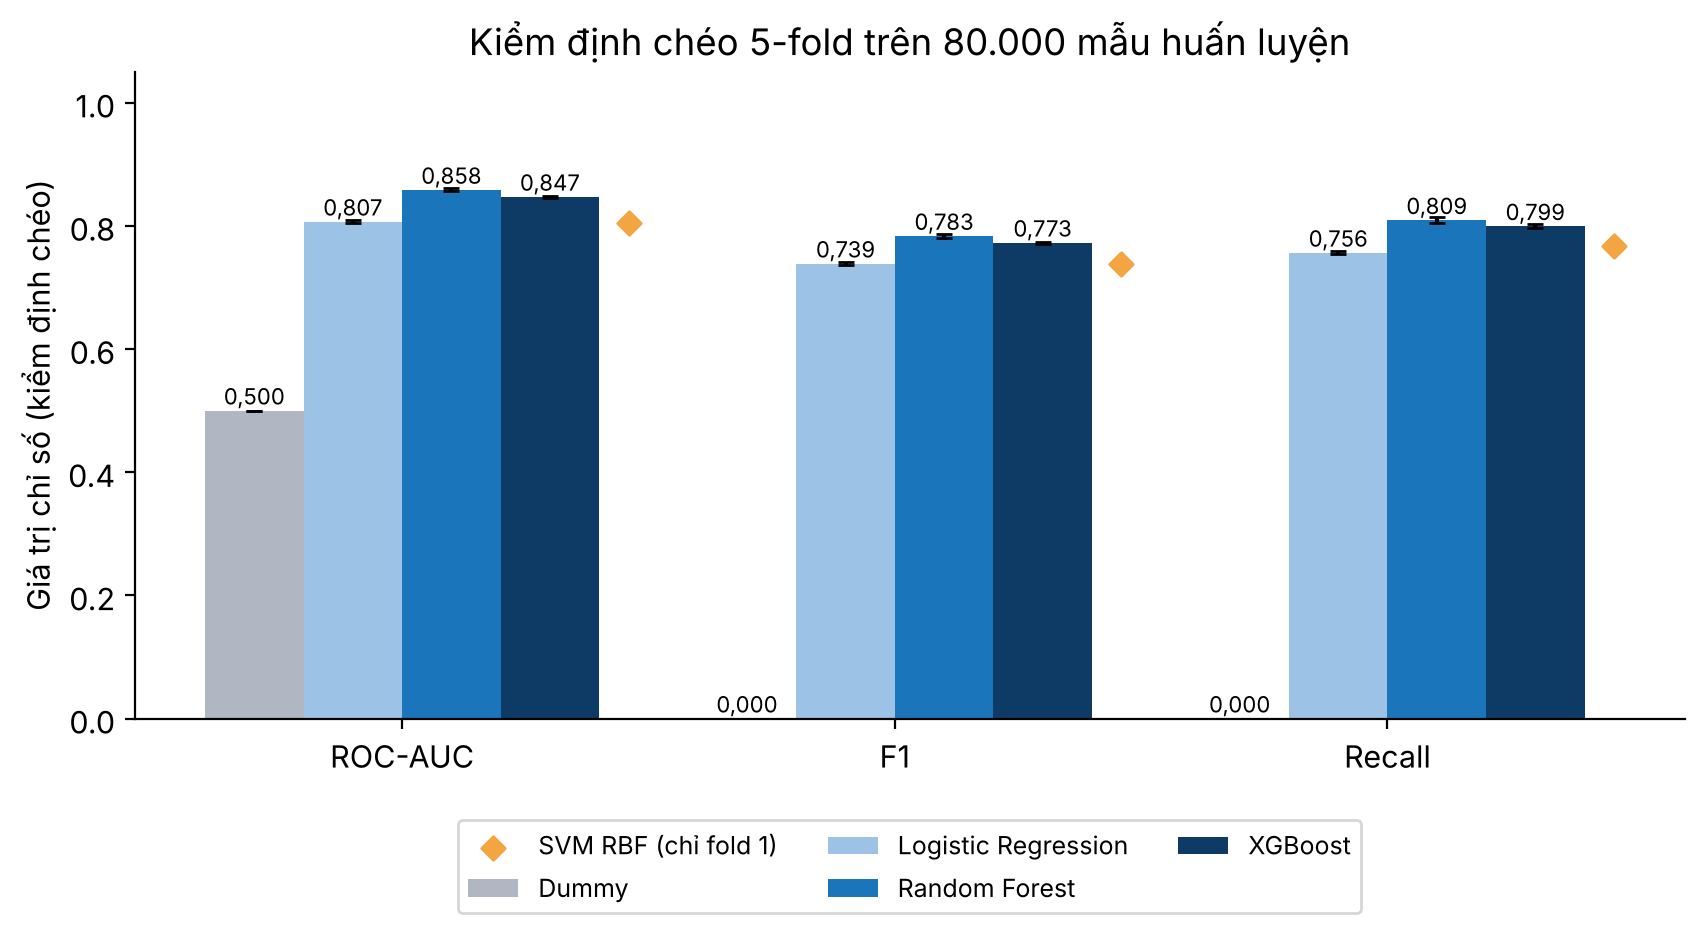
\includegraphics[width=0.9\textwidth]{fig09_cv_so_sanh.png}
  \caption{So sánh các mô hình bằng kiểm định chéo 5-fold (thanh lỗi: độ lệch chuẩn qua 5 fold)}
  \label{fig:cv5}
\end{figure}

\textit{Nhận xét} (Bảng~\ref{tab:cv5}, Hình~\ref{fig:cv5}):
\begin{itemize}
  \item Cả ba mô hình đều vượt xa mô hình cơ sở Dummy (ROC-AUC 0,5). Mô hình
        Dummy chỉ dự đoán một lớp nên F1 bằng 0 (khi dự đoán toàn lớp 0); đây
        là mốc ``không học gì''.
  \item Random Forest tốt nhất ở mọi chỉ số (ROC-AUC 0,858, F1 0,783),
        hơn XGBoost cấu hình mặc định khoảng 0,011 ROC-AUC và hơn Logistic
        Regression 0,051. Khoảng cách giữa RF và XGBoost lớn gấp khoảng 5 lần độ
        lệch chuẩn giữa các fold, nên chênh lệch là ổn định, không do may rủi
        của cách chia.
  \item Độ lệch chuẩn qua 5 fold rất nhỏ (0,002--0,003), cho thấy với 16.000 mẫu
        kiểm định mỗi fold, ước lượng hiệu năng đã ổn định.
  \item Mô hình tuyến tính kém hơn rõ rệt mô hình cây, khớp với nhận xét ở
        Mục~\ref{sec:quanhe}: tín hiệu nằm ở tổ hợp nhiều bit, cần mô
        hình phi tuyến.
\end{itemize}

\subsection{SVM nhân RBF trên fold 1}
Huấn luyện SVM trên 64.000 mẫu của một fold mất vài giờ (độ phức tạp xấp xỉ bậc
hai theo số mẫu), nên SVM được huấn luyện trên 20.000 mẫu lấy phân tầng từ phần
huấn luyện của fold 1 và đánh giá trên toàn bộ phần kiểm định của fold 1
(16.000 mẫu), cùng phần kiểm định với các mô hình khác (Bảng~\ref{tab:svm}).

\begin{table}[H]
  \centering
  \caption{So sánh trên fold 1 (cùng 16.000 mẫu kiểm định)}
  \label{tab:svm}
  \small
  \begin{tabular}{lccccrr}
    \toprule
    \textbf{Mô hình} & \textbf{Số mẫu học} & \textbf{ROC-AUC} & \textbf{F1} & \textbf{Recall} & \textbf{AUC train} & \textbf{Fit (s)} \\
    \midrule
    Logistic Regression & 64.000 & 0,807 & 0,737 & 0,755 & 0,837 & 23,8 \\
    Random Forest & 64.000 & 0,860 & 0,785 & 0,810 & 1,000 & 86,3 \\
    XGBoost & 64.000 & 0,848 & 0,773 & 0,800 & 0,928 & 45,1 \\
    SVM (RBF, $C=1$) & 20.000 & 0,804 & 0,738 & 0,767 & 0,969 & 462,9 \\
    \bottomrule
  \end{tabular}
\end{table}

\textit{Nhận xét:} SVM học trên 20.000 mẫu mất 463 giây, lâu gấp 5 lần Random
Forest học trên 64.000 mẫu, nhưng chỉ đạt ROC-AUC 0,804, tương đương Logistic
Regression và kém Random Forest 0,056. SVM giữ lại 16.739 vectơ hỗ trợ (84\% số
mẫu học), nghĩa là biên phân tách rất phức tạp. Với dữ liệu lớn và đặc trưng nhị
phân thưa như bài toán này, SVM nhân RBF không phù hợp về chi phí, nên nhóm không
đưa SVM vào các bước tối ưu tiếp theo.

\subsection{Đánh giá trên tập kiểm tra}
\begin{table}[H]
  \centering
  \caption{Kết quả trên tập kiểm tra giữ lại (20.000 cặp, huấn luyện trên toàn bộ 80.000 mẫu)}
  \label{tab:test2}
  \small
  \begin{tabular}{lccccc}
    \toprule
    \textbf{Mô hình} & \textbf{ROC-AUC} & \textbf{F1} & \textbf{Recall} & \textbf{Precision} & \textbf{Accuracy} \\
    \midrule
    Dummy & 0,500 & 0,667$^{*}$ & 1,000$^{*}$ & 0,500 & 0,500 \\
    Logistic Regression & 0,812 & 0,744 & 0,765 & 0,723 & 0,736 \\
    Random Forest & 0,865 & 0,789 & 0,822 & 0,759 & 0,780 \\
    XGBoost & 0,853 & 0,779 & 0,810 & 0,751 & 0,771 \\
    \bottomrule
    \multicolumn{6}{l}{\footnotesize $^{*}$ Dummy cho xác suất 0,5 với mọi cặp; ở ngưỡng $\geq 0{,}5$ mọi cặp bị gán lớp 1.}
  \end{tabular}
\end{table}

\begin{figure}[H]
  \centering
  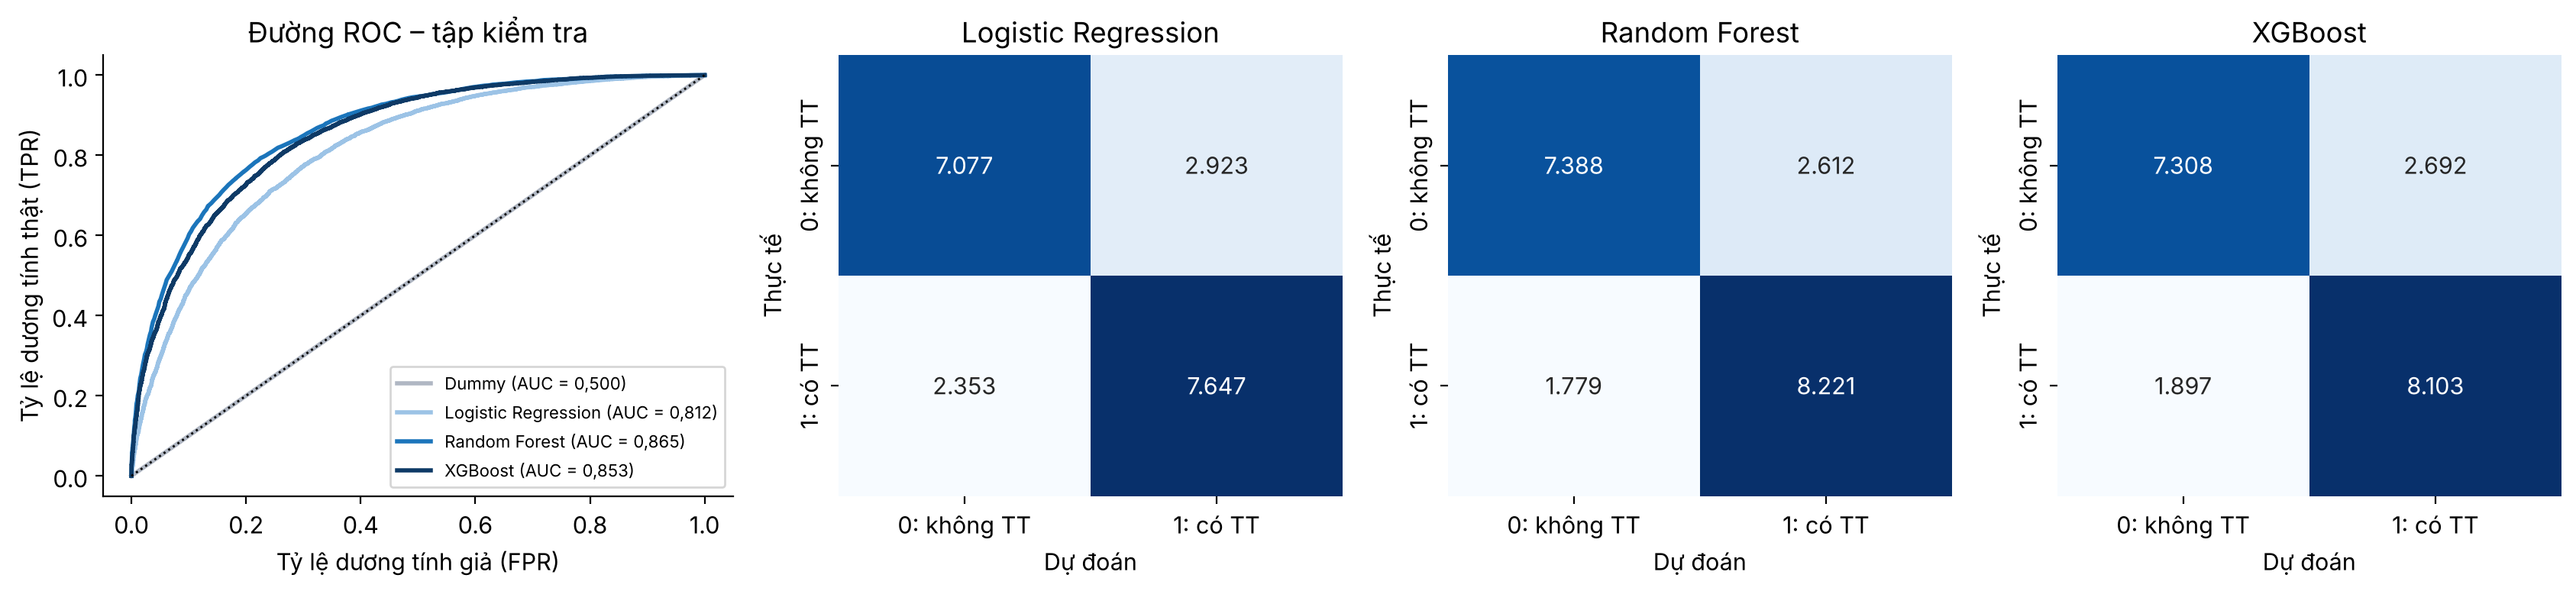
\includegraphics[width=\textwidth]{fig10_roc_nham_lan.png}
  \caption{Đường ROC và ma trận nhầm lẫn trên tập kiểm tra (ngưỡng 0,5)}
  \label{fig:rocnhamlan}
\end{figure}

\textit{Nhận xét} (Bảng~\ref{tab:test2}, Hình~\ref{fig:rocnhamlan}):
\begin{itemize}
  \item Thứ hạng trên tập kiểm tra giống hệt kiểm định chéo (RF $>$ XGBoost $>$
        LR $>$ Dummy) và các giá trị chỉ chênh 0,005--0,007 so với kiểm định
        chéo, nên kết quả kiểm định chéo đáng tin cậy.
  \item Đường ROC của RF và XGBoost gần như trùng nhau, cùng nằm trên LR ở mọi
        ngưỡng. Khi chỉ chấp nhận 10\% báo động sai (FPR $=0{,}1$), RF phát hiện
        60\% số cặp có tương tác, XGBoost 55\%, LR 46\%.
  \item Random Forest bỏ sót 1.779 cặp có tương tác (FN) và báo động sai 2.612
        cặp (FP): mô hình nghiêng về phía dự đoán ``có tương tác'' (Recall 0,822
        cao hơn Precision 0,759), phù hợp với ưu tiên không bỏ sót trong an
        toàn thuốc.
  \item So với mục tiêu ở Bảng~\ref{tab:muctieu}: RF và XGBoost đạt ROC-AUC
        $\geq 0{,}85$ và Recall $\geq 0{,}80$; F1 cao nhất 0,789 chưa đạt
        mục tiêu 0,80.
\end{itemize}

\section{Phân tích kết quả dự đoán và đặc trưng quan trọng}
\label{sec:phantichloi}


\subsection{Quá khớp và chưa khớp}
\begin{table}[H]
  \centering
  \caption{ROC-AUC trên phần huấn luyện và phần kiểm định (trung bình 5 fold)}
  \label{tab:gap}
  \small
  \begin{tabular}{lccc}
    \toprule
    \textbf{Mô hình} & \textbf{Huấn luyện} & \textbf{Kiểm định} & \textbf{Chênh lệch} \\
    \midrule
    Logistic Regression & 0,837 & 0,807 & 0,030 \\
    Random Forest & 1,000 & 0,858 & 0,142 \\
    XGBoost & 0,928 & 0,847 & 0,081 \\
    \bottomrule
  \end{tabular}
\end{table}

\textit{Nhận xét:} Logistic Regression có chênh lệch nhỏ nhưng điểm huấn luyện
cũng thấp (0,837): mô hình chưa khớp (độ chệch cao), không đủ khả năng
biểu diễn tương tác giữa các bit. Random Forest khớp hoàn hảo tập huấn luyện
(ROC-AUC 1,000) vì các cây được phát triển hết độ sâu: đây là quá khớp,
nhưng nhờ lấy trung bình 300 cây nên hiệu năng kiểm định vẫn cao nhất. XGBoost
nằm giữa (chênh lệch 0,081). Như vậy hạn chế chính của mô hình ban đầu là quá
khớp ở mô hình cây, sẽ được xử lý ở Mục~\ref{sec:hanche2} và~\ref{sec:caitien}.

\subsection{Lỗi tập trung ở nhóm dữ liệu nào}
Phân tích trên tập kiểm tra với Random Forest (mô hình tốt nhất). Bậc của thuốc
chỉ dùng để phân tích, không đưa vào mô hình.

\begin{figure}[H]
  \centering
  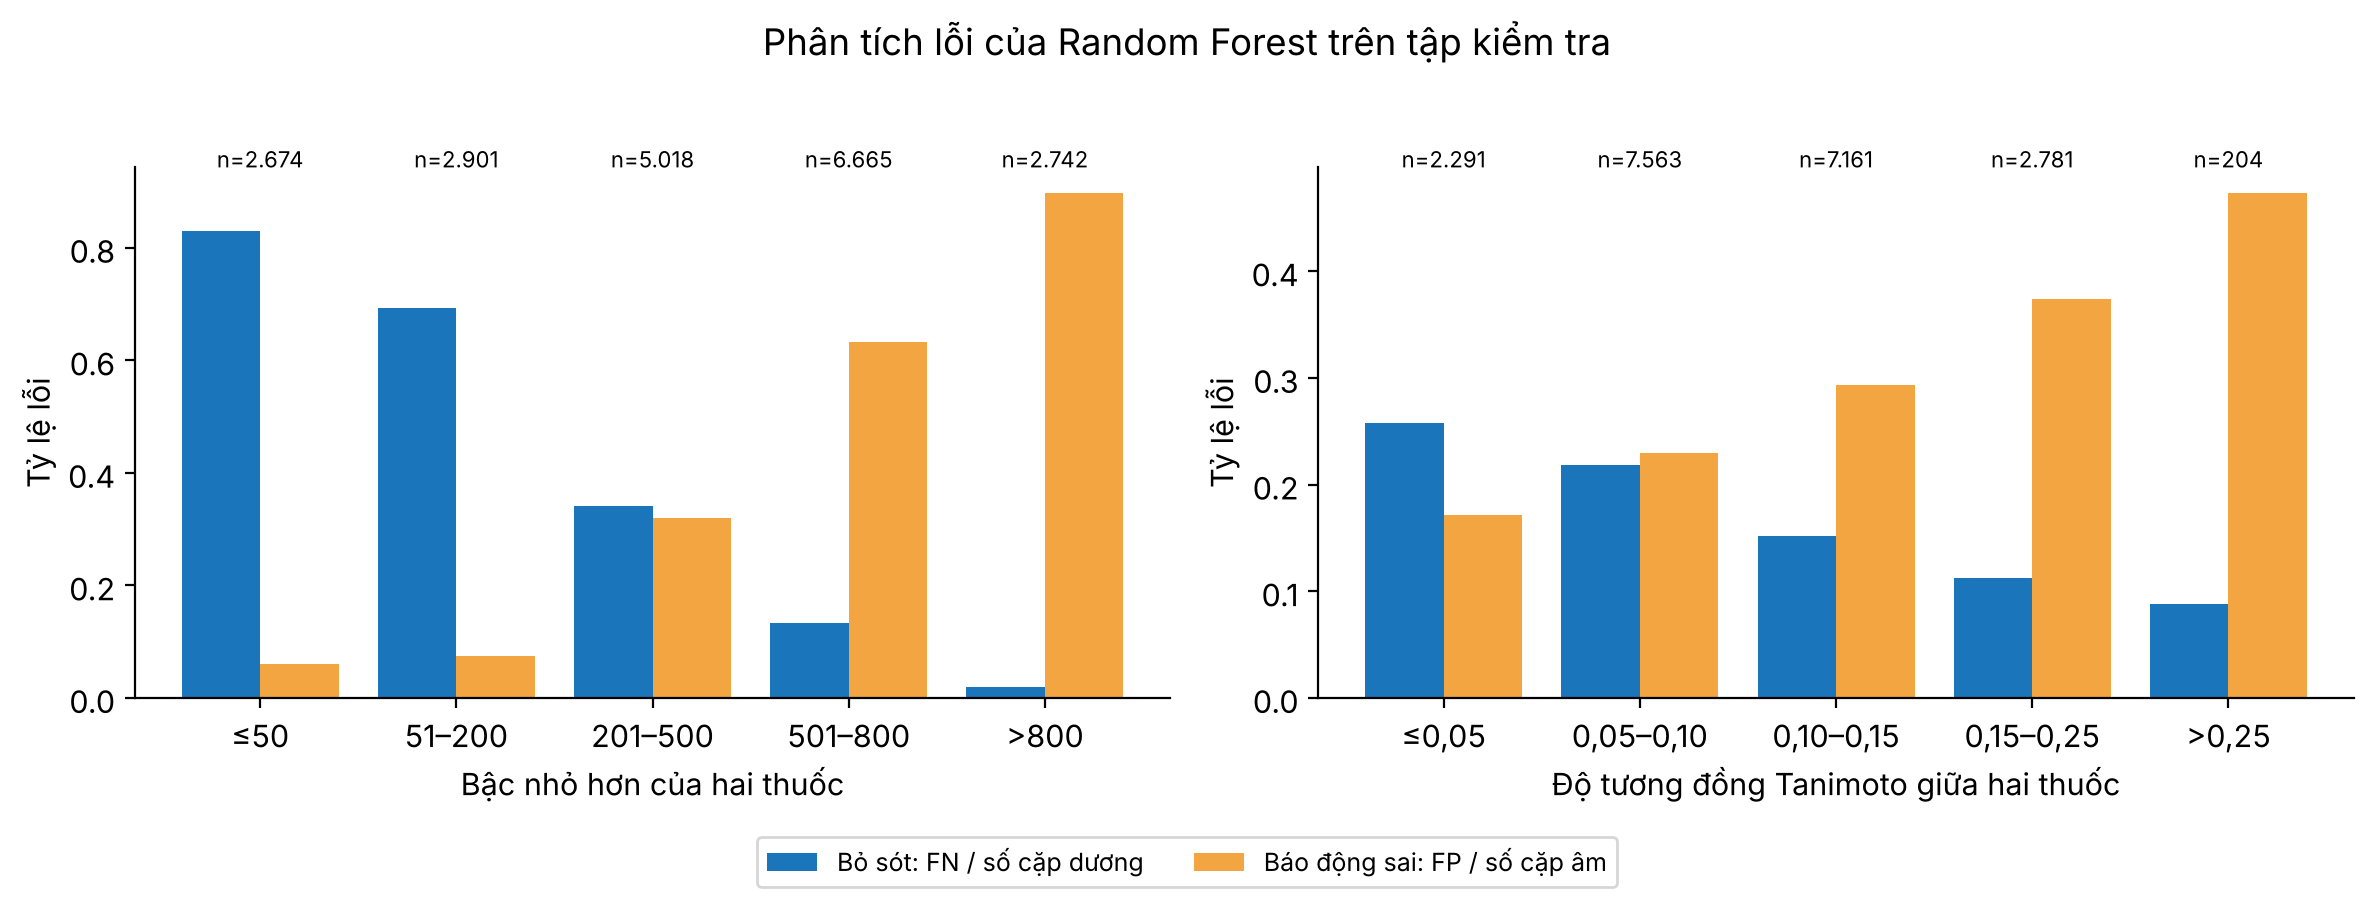
\includegraphics[width=\textwidth]{fig11_phan_tich_loi.png}
  \caption{Tỷ lệ bỏ sót (FN/số cặp dương) và báo động sai (FP/số cặp âm) của Random Forest theo bậc và theo độ tương đồng cấu trúc}
  \label{fig:phantichloi}
\end{figure}

\begin{table}[H]
  \centering
  \caption{Lỗi của Random Forest theo bậc nhỏ hơn của hai thuốc (tập kiểm tra)}
  \label{tab:loibac}
  \small
  \begin{tabular}{lrcccc}
    \toprule
    \textbf{Bậc nhỏ hơn} & \textbf{Số cặp} & \textbf{Tỷ lệ dương} & \textbf{Tỷ lệ sai} & \textbf{FN/dương} & \textbf{FP/âm} \\
    \midrule
    $\leq 50$ & 2.674 & 0,022 & 0,077 & 0,831 & 0,060 \\
    51--200 & 2.901 & 0,154 & 0,170 & 0,693 & 0,075 \\
    201--500 & 5.018 & 0,430 & 0,328 & 0,341 & 0,319 \\
    501--800 & 6.665 & 0,719 & 0,273 & 0,133 & 0,632 \\
    $> 800$ & 2.742 & 0,929 & 0,082 & 0,019 & 0,898 \\
    \bottomrule
  \end{tabular}
\end{table}

\textit{Nhận xét} (Hình~\ref{fig:phantichloi}, Bảng~\ref{tab:loibac}):
\begin{itemize}
  \item Lỗi phụ thuộc mạnh vào độ phổ biến của thuốc. Với cặp có một
        thuốc ít tương tác (bậc $\leq 50$), mô hình bỏ sót 83\% số cặp có tương
        tác; với cặp gồm hai thuốc rất phổ biến (bậc $> 800$), mô hình báo động
        sai 90\% số cặp không tương tác. Mô hình đã học được ``thuốc này hay
        tương tác'' từ vân tay thay vì quan hệ giữa hai cấu trúc, đúng với thiên
        lệch dự báo ở Mục~\ref{sec:chatluong}.
  \item Lỗi nhiều nhất ở nhóm bậc trung bình (201--500, tỷ lệ sai 32,8\%) vì
        đây là nhóm có hai lớp cân bằng nhất, mô hình không dựa được vào độ
        phổ biến.
  \item Theo độ tương đồng Tanimoto, hai thuốc càng giống nhau thì tỷ lệ báo
        động sai càng tăng (17\% $\rightarrow$ 47\%) và tỷ lệ bỏ sót càng giảm
        (26\% $\rightarrow$ 9\%): mô hình có xu hướng cho rằng hai thuốc cấu trúc
        giống nhau thì tương tác.
  \item Các thuốc bị dự đoán sai nhiều nhất (trong các thuốc xuất hiện ở ít
        nhất 30 cặp) là Celecoxib (40\% số cặp sai), Ponatinib (36,7\%), Dimethyl
        sulfoxide (35,5\%), Benzocaine (32,3\%) -- đều là thuốc có bậc cao
        (781--1.260), xuất hiện nhiều ở cả mẫu dương lẫn mẫu âm.
\end{itemize}

\subsection{Đặc trưng ảnh hưởng nhiều đến dự đoán}
\begin{figure}[H]
  \centering
  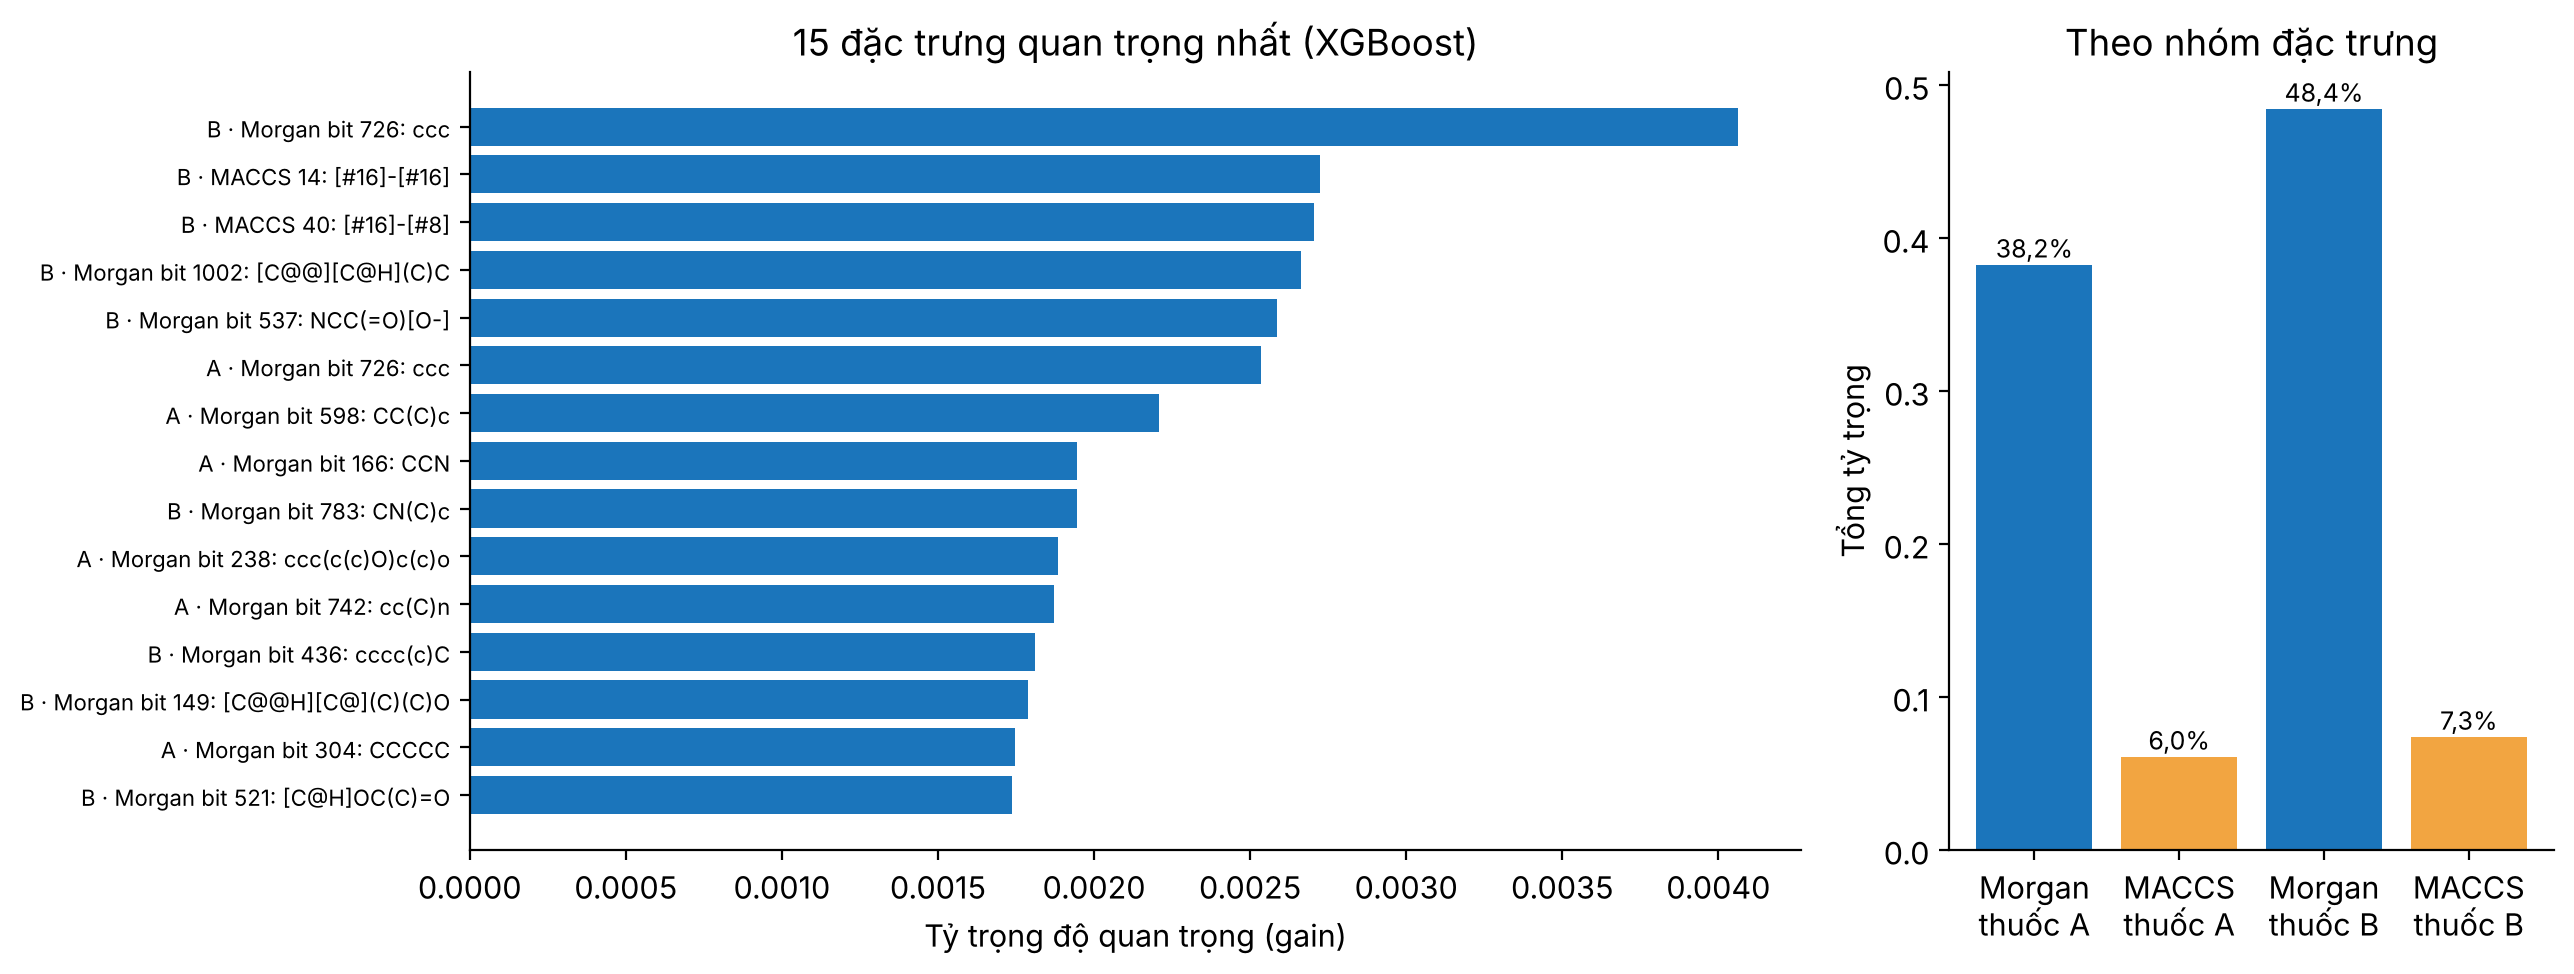
\includegraphics[width=\textwidth]{fig12_dac_trung_quan_trong.png}
  \caption{Độ quan trọng đặc trưng của XGBoost (theo gain): 15 đặc trưng lớn nhất và tổng theo nhóm}
  \label{fig:dactrung}
\end{figure}

\textit{Nhận xét} (Hình~\ref{fig:dactrung}):
\begin{itemize}
  \item Vân tay Morgan chiếm 86,6\% tổng độ quan trọng, MACCS chỉ 13,4\%. Morgan
        mô tả chi tiết các mảnh cấu trúc nên mang nhiều thông tin hơn 166 khóa
        MACCS định sẵn.
  \item Độ quan trọng phân tán: 15 đặc trưng lớn nhất chỉ chiếm 3,4\% tổng, nghĩa
        là mô hình dựa vào tổ hợp của rất nhiều bit, khớp với nhận xét mỗi bit
        riêng lẻ chỉ liên quan yếu đến nhãn.
  \item Các đặc trưng đứng đầu là mảnh vòng thơm (Morgan bit 726, \texttt{ccc}),
        liên kết lưu huỳnh -- lưu huỳnh và lưu huỳnh -- oxy (MACCS 14, 40), nhóm
        amin gắn vòng thơm (\texttt{CN(C)c}). Các bit Morgan bị băm vào 1.024 vị
        trí nên một bit có thể ứng với nhiều mảnh khác nhau; mảnh ghi trong hình
        là mảnh hay gặp nhất làm bật bit đó.
  \item Độ quan trọng không đối xứng: các bit của thuốc B chiếm 55,8\%, thuốc A
        chỉ 44,3\%, dù vai trò hai thuốc trong một cặp là như nhau. Mô hình phụ
        thuộc vào thứ tự ghép nối (A là thuốc có mã nhỏ hơn) -- một hạn chế của
        cách biểu diễn ban đầu, được phân tích ở Mục~\ref{sec:hanche2}.
\end{itemize}

\subsection{Giải thích vì sao mô hình này tốt hơn mô hình kia}
\begin{itemize}
  \item Random Forest $>$ Logistic Regression: LR chỉ cộng tuyến tính
        ảnh hưởng của từng bit, trong khi tương tác thuốc phụ thuộc vào việc
        đồng thời có những mảnh cấu trúc nhất định ở cả hai thuốc. Mỗi
        đường đi từ gốc đến lá của cây là một tổ hợp điều kiện trên nhiều bit,
        nên cây biểu diễn được các tương tác này.
  \item Random Forest $>$ XGBoost (cấu hình ban đầu): với 2.382 đặc
        trưng nhị phân thưa và nhiều nhiễu nhãn (mẫu âm là cặp chưa ghi
        nhận), việc lấy trung bình nhiều cây sâu độc lập của RF bền vững hơn.
        XGBoost với độ sâu 6 bị giới hạn mức tương tác giữa các bit mà mỗi cây
        biểu diễn được, nên cần tinh chỉnh siêu tham số (Mục~\ref{sec:caitien}).
  \item SVM kém và chậm: khoảng cách Euclid trên vectơ nhị phân thưa
        2.382 chiều ít ý nghĩa với nhân RBF; lại chỉ học được 20.000 mẫu.
\end{itemize}

\section{Phân tích hạn chế và đề xuất giải pháp}
\label{sec:hanche2}

Các thí nghiệm từ mục này trở đi nằm trong notebook
\texttt{03\_ToiUu\_CaiTien.ipynb}. Trước khi cải tiến, cần xác định mô hình ban
đầu yếu ở đâu và đưa ra bằng chứng định lượng cho từng hạn chế.

\subsection{Phân tích hạn chế của mô hình ban đầu}

\begin{figure}[H]
  \centering
  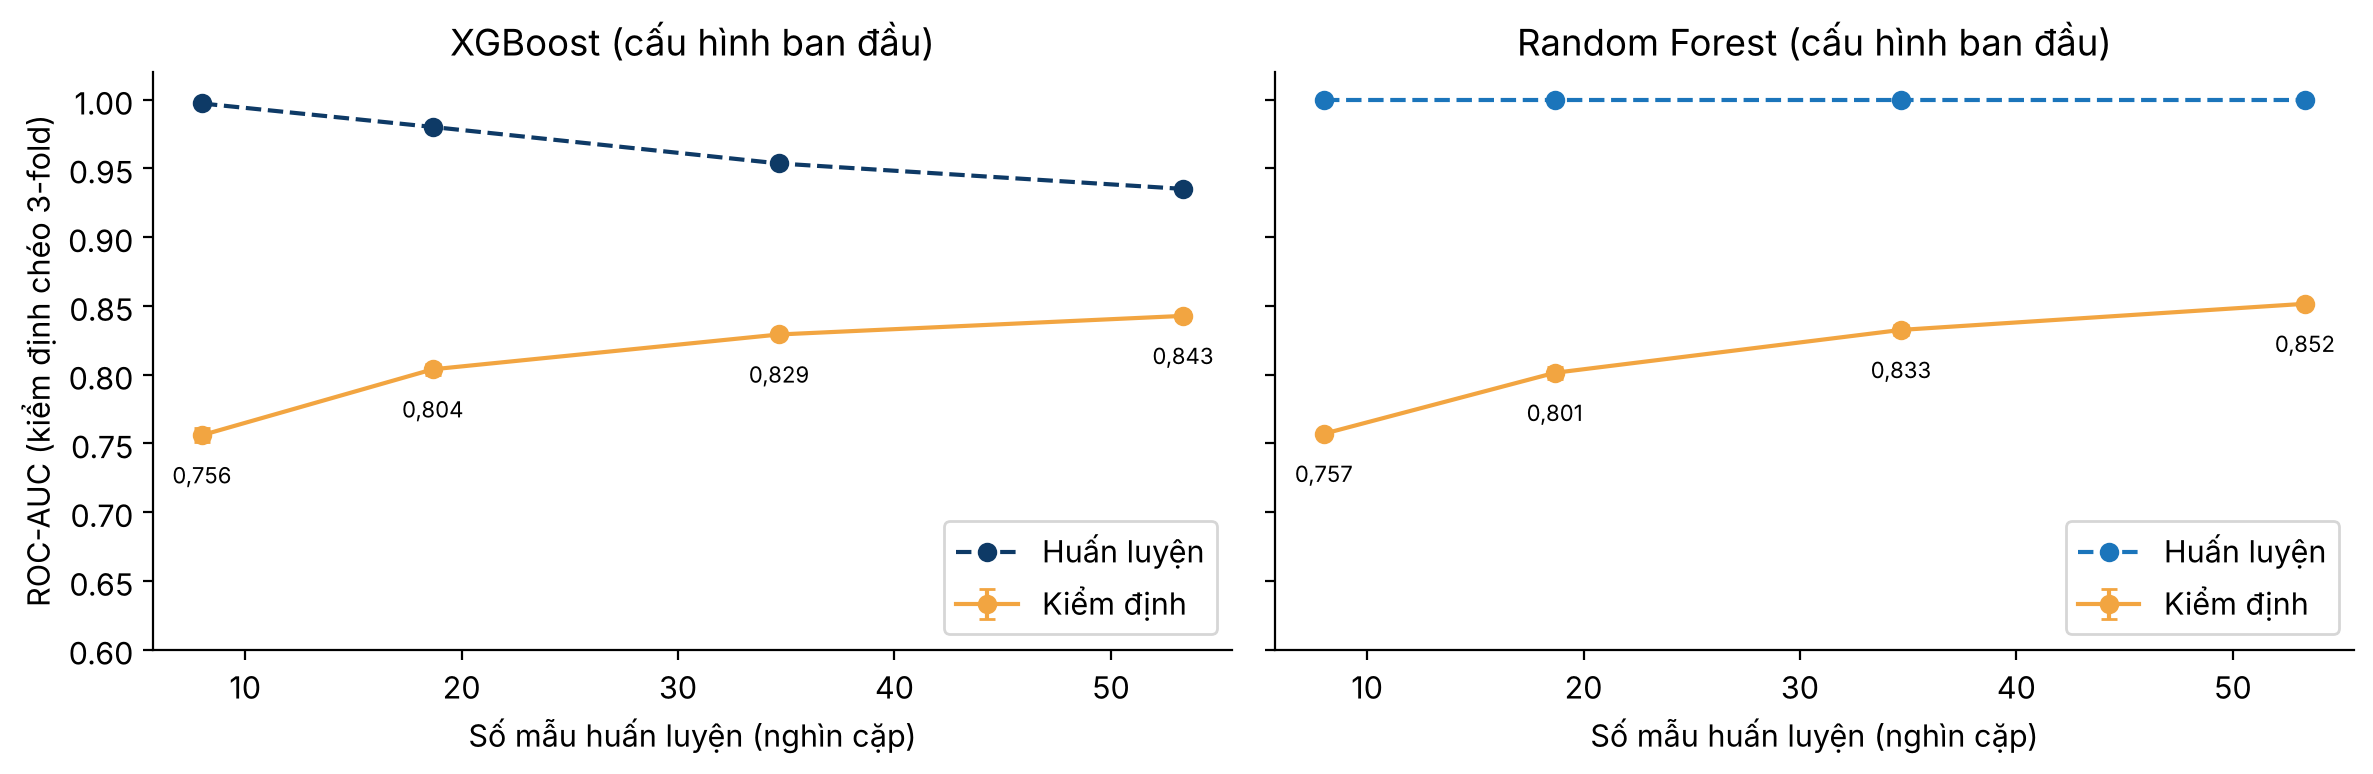
\includegraphics[width=0.95\textwidth]{fig13_duong_cong_hoc.png}
  \caption{Đường cong học tập của XGBoost và Random Forest (cấu hình ban đầu, kiểm định chéo 3-fold)}
  \label{fig:duongconghoc}
\end{figure}

\textit{Nhận xét} (Hình~\ref{fig:duongconghoc}): Random Forest luôn đạt ROC-AUC
huấn luyện bằng 1,000, còn ROC-AUC kiểm định tăng từ 0,757 (8.000 mẫu) lên 0,852
(53.333 mẫu); XGBoost tăng từ 0,756 lên 0,843 trong khi điểm huấn luyện giảm dần
từ 0,997 xuống 0,935. Khoảng cách huấn luyện -- kiểm định lớn (0,09--0,15) và
đường kiểm định chưa đi ngang ở cuối: mô hình đang ở chế độ phương sai cao,
sẽ có lợi khi có thêm dữ liệu hoặc khi được điều chuẩn tốt hơn.

\begin{figure}[H]
  \centering
  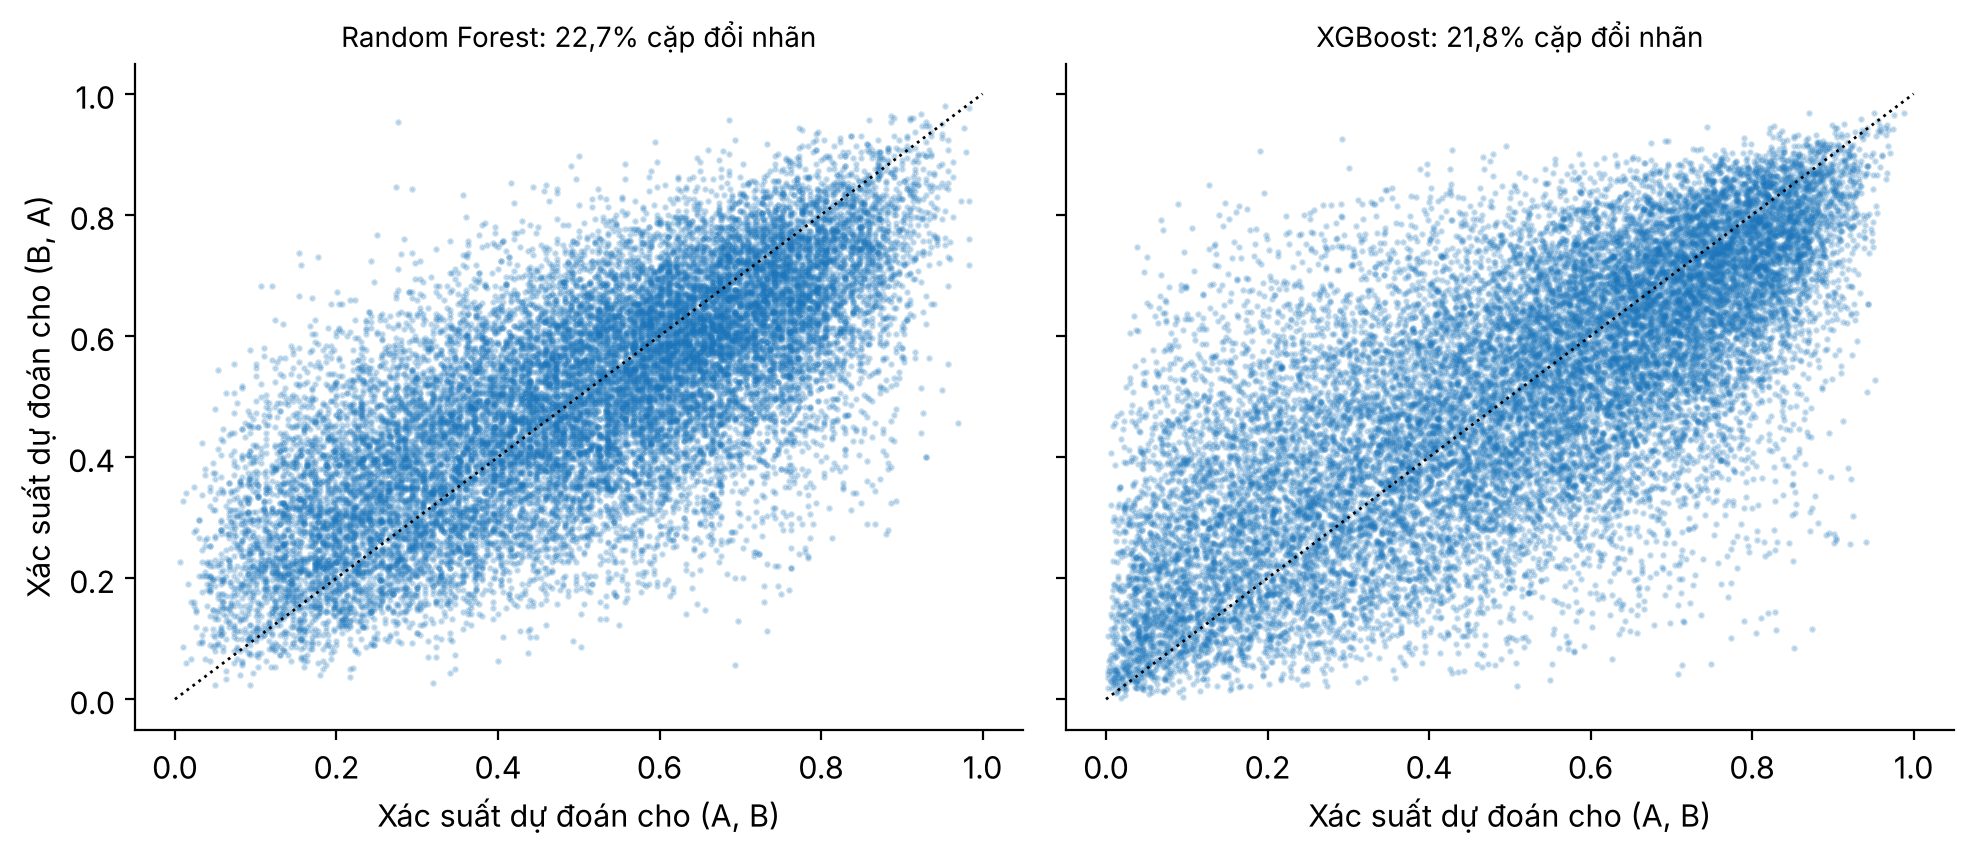
\includegraphics[width=0.82\textwidth]{fig14_thu_tu_cap.png}
  \caption{Xác suất dự đoán của mô hình ban đầu khi đổi thứ tự hai thuốc trong cặp (tập kiểm tra)}
  \label{fig:thutucap}
\end{figure}

\textit{Nhận xét} (Hình~\ref{fig:thutucap}): cặp $(A,B)$ và $(B,A)$ là cùng một cặp
thuốc nhưng mô hình ban đầu cho hai xác suất khác nhau: trung bình lệch 0,120 (RF)
và 0,134 (XGBoost); 22,7\% (RF) và 21,8\% (XGBoost) số cặp bị đổi nhãn dự
đoán khi đổi chỗ. ROC-AUC của RF giảm từ 0,865 xuống 0,796 khi đưa vào thứ tự
ngược. Lý do: thuốc $A$ luôn là thuốc có mã DrugBank nhỏ hơn, tức thường là thuốc
cũ hơn; mã thuốc tương quan âm với số tương tác (Spearman $\rho=-0{,}37$), nên vị
trí trong vectơ vô tình mang thông tin về độ phổ biến của thuốc.

Ngoài ra, khi đánh giá trên thuốc mới (huấn luyện trên 63.756 cặp chỉ gồm thuốc
đã biết), ROC-AUC của RF giảm từ 0,858 xuống 0,799 khi cặp có một thuốc mới (S1)
và 0,720 khi cả hai thuốc đều mới (S2); XGBoost giảm còn 0,774 và 0,680. Cùng với
phân tích lỗi ở Mục~\ref{sec:phantichloi} (lỗi phụ thuộc mạnh vào bậc của thuốc),
có thể kết luận mô hình ban đầu dựa một phần vào ``độ phổ biến'' của thuốc thay
vì quan hệ cấu trúc giữa hai thuốc.

\subsection{Đề xuất giải pháp}

\begin{table}[H]
  \centering
  \caption{Các hạn chế, bằng chứng và giải pháp đề xuất}
  \label{tab:hanche}
  \small
  \begin{tabularx}{\textwidth}{>{\raggedright\arraybackslash}p{4.2cm} >{\raggedright\arraybackslash}X >{\raggedright\arraybackslash}p{4.3cm}}
    \toprule
    \textbf{Hạn chế (bằng chứng)} & \textbf{Giải pháp} & \textbf{Cơ sở lý thuyết} \\
    \midrule
    H1. Dự đoán phụ thuộc thứ tự $A/B$: 22,7\% cặp đổi nhãn (Hình~\ref{fig:thutucap}); độ quan trọng lệch về thuốc $B$ (55,8\%) &
      (a) Dự đoán hai chiều: lấy trung bình xác suất của $(A,B)$ và $(B,A)$. (b) Biểu diễn đối xứng $\mathrm{FP}(A)+\mathrm{FP}(B)$, 1.191 chiều &
      Cặp không thứ tự cần hàm dự đoán đối xứng $f(A,B)=f(B,A)$; giảm một nửa số chiều \\
    H2. Vân tay nhị phân bỏ mất số lần xuất hiện của mảnh cấu trúc và tính chất hóa lý &
      Morgan dạng đếm (cộng hai thuốc) + MACCS + 9 đặc trưng hóa lý (tổng và $|$hiệu$|$ của khối lượng, LogP, TPSA\dots) &
      Tương tác dược động học phụ thuộc độ ưa béo, kích thước, số nhóm chức \\
    H3. Quá khớp: RF train 1,000; XGBoost chênh 0,081; siêu tham số mặc định (Hình~\ref{fig:duongconghoc}) &
      Random Search trên kiểm định chéo: độ sâu, số cây, tốc độ học, điều chuẩn L2, tỷ lệ lấy mẫu &
      Đánh đổi độ chệch -- phương sai; điều chuẩn hạn chế quá khớp \\
    H4. Mỗi mô hình đơn lẻ có phương sai riêng &
      Thuật toán mới Extra Trees; tổ hợp Soft Voting RF + XGBoost &
      Ngẫu nhiên hóa và kết hợp mô hình có lỗi khác nhau làm giảm phương sai \\
    H5. Lỗi tập trung theo bậc thuốc; giảm mạnh với thuốc mới &
      Thí nghiệm lấy mẫu âm cân bằng theo bậc để đo phần hiệu năng đến từ độ phổ biến &
      Loại ``lối tắt'' (shortcut) do cách lấy mẫu âm \\
    \bottomrule
  \end{tabularx}
\end{table}

\section{Cải tiến đặc trưng, tối ưu siêu tham số và thuật toán mới}
\label{sec:caitien}

\subsection{Cải tiến đặc trưng}
Mỗi cách biểu diễn được đánh giá với siêu tham số mặc định như Bài kiểm tra 2, cùng
5 fold (Bảng~\ref{tab:caitiendactrung}).

\begin{table}[H]
  \centering
  \caption{ROC-AUC kiểm định chéo 5-fold theo cách biểu diễn cặp thuốc (siêu tham số mặc định)}
  \label{tab:caitiendactrung}
  \small
  \begin{tabular}{lcccc}
    \toprule
    \textbf{Biểu diễn} & \textbf{Số chiều} & \textbf{LR} & \textbf{RF} & \textbf{XGBoost} \\
    \midrule
    Ghép nối (ban đầu) & 2.382 & 0,807 & 0,858 & 0,847 \\
    Ghép nối + dự đoán hai chiều & 2.382 & 0,784 & 0,854 & 0,838 \\
    Đối xứng $\mathrm{FP}(A)+\mathrm{FP}(B)$ & 1.191 & 0,793 & 0,851 & 0,853 \\
    Đối xứng + Morgan đếm + hóa lý & 1.209 & 0,803 & 0,845 & 0,854 \\
    \bottomrule
    \multicolumn{5}{l}{\footnotesize Độ lệch chuẩn qua 5 fold: 0,002--0,003 cho mọi ô.}
  \end{tabular}
\end{table}

\textit{Nhận xét} (Bảng~\ref{tab:caitiendactrung}):
\begin{itemize}
  \item Dự đoán hai chiều không hiệu quả với cả ba mô hình (giảm
        0,004--0,023). Mô hình được huấn luyện với thuốc có mã nhỏ luôn ở vị trí
        $A$, nên vectơ đổi chỗ là dữ liệu ``lạ'' với nó; lấy trung bình với một dự
        đoán kém hơn làm giảm chất lượng. Muốn đối xứng thật sự cần huấn luyện trên
        cả hai thứ tự (nhân đôi dữ liệu), nhưng với Random Forest cách này cần hơn
        6~GB RAM, vượt khả năng máy của nhóm.
  \item Biểu diễn đối xứng có lợi cho XGBoost (0,847 $\rightarrow$ 0,853,
        +0,006, gấp khoảng 3 lần độ lệch chuẩn) nhưng bất lợi cho RF
        (0,858 $\rightarrow$ 0,851). Với XGBoost độ sâu 6, mỗi cây chỉ biểu diễn
        được ít tương tác; biểu diễn tổng gộp thông tin ``mảnh cấu trúc có ở một
        hay cả hai thuốc'' (giá trị 0/1/2) vào một đặc trưng nên dễ khai thác hơn.
        RF dùng cây sâu tối đa, khai thác được cả thông tin vị trí (gồm cả độ phổ
        biến ngầm theo mã thuốc ở trên), nên mất thông tin này thì giảm điểm.
  \item Morgan dạng đếm + đặc trưng hóa lý tăng thêm cho LR (+0,010) và
        XGBoost (+0,0003), giảm cho RF. Biểu diễn tốt nhất của XGBoost là
        ``đối xứng + đếm + hóa lý'', của RF vẫn là ghép nối; các mô hình được tối
        ưu tiếp trên biểu diễn tốt nhất của chính nó.
\end{itemize}

\subsection{Tối ưu hóa siêu tham số}
Mỗi mô hình được tối ưu bằng Random Search (\texttt{ParameterSampler},
\texttt{random\_state = 42}) với kiểm định chéo phân tầng 3-fold. Do giới hạn
thời gian trên CPU 2 nhân, việc tìm kiếm chạy trên 30.000 mẫu lấy phân tầng từ
tập huấn luyện; cấu hình tốt nhất sau đó được đánh giá lại bằng kiểm định chéo
5-fold trên toàn bộ 80.000 mẫu. Tập kiểm tra không tham gia vào việc chọn siêu
tham số. Không gian tìm kiếm và kết quả ở Bảng~\ref{tab:sieuthamso}.

\begin{table}[H]
  \centering
  \caption{Không gian tìm kiếm và siêu tham số tối ưu}
  \label{tab:sieuthamso}
  \small
  \begin{tabularx}{\textwidth}{l >{\raggedright\arraybackslash}X >{\raggedright\arraybackslash}p{3.2cm}}
    \toprule
    \textbf{Siêu tham số} & \textbf{Không gian tìm kiếm} & \textbf{Giá trị tối ưu} \\
    \midrule
    \multicolumn{3}{l}{\textit{XGBoost (biểu diễn đối xứng + đếm + hóa lý), 10 cấu hình $\times$ 3 fold, 527 giây}} \\
    \texttt{n\_estimators} & số nguyên 300--900 & 608 \\
    \texttt{max\_depth} & \{4, 6, 8, 10\} & 10 \\
    \texttt{learning\_rate} & log-đều 0,02--0,2 & 0,147 \\
    \texttt{subsample} & đều 0,6--1,0 & 0,933 \\
    \texttt{colsample\_bytree} & đều 0,3--0,9 & 0,335 \\
    \texttt{min\_child\_weight} & \{1, 3, 5\} & 5 \\
    \texttt{reg\_lambda} & log-đều 0,5--10 & 9,14 \\
    \midrule
    \multicolumn{3}{l}{\textit{Random Forest (biểu diễn ghép nối), 6 cấu hình $\times$ 3 fold, 1.221 giây}} \\
    \texttt{n\_estimators} & \{300, 500\} & 500 \\
    \texttt{max\_features} & \{sqrt, 0,05, 0,1\} & 0,1 \\
    \texttt{min\_samples\_leaf} & \{1, 2, 4\} & 1 \\
    \texttt{max\_depth} & \{không giới hạn, 40\} & không giới hạn \\
    \bottomrule
  \end{tabularx}
\end{table}

Trên tập con 30.000 mẫu (3-fold), ROC-AUC của XGBoost tăng từ 0,821 (mặc định)
lên 0,833; của RF tăng từ 0,805 lên 0,809. Ba cấu hình XGBoost tốt nhất đều có
cây sâu (8--10), điều chuẩn L2 mạnh (\texttt{reg\_lambda} $\approx 7$--$9$) và chỉ
dùng khoảng 1/3 số đặc trưng cho mỗi cây; các cấu hình nông (độ sâu 4--6) cho kết
quả kém nhất (0,780--0,821).

\begin{figure}[H]
  \centering
  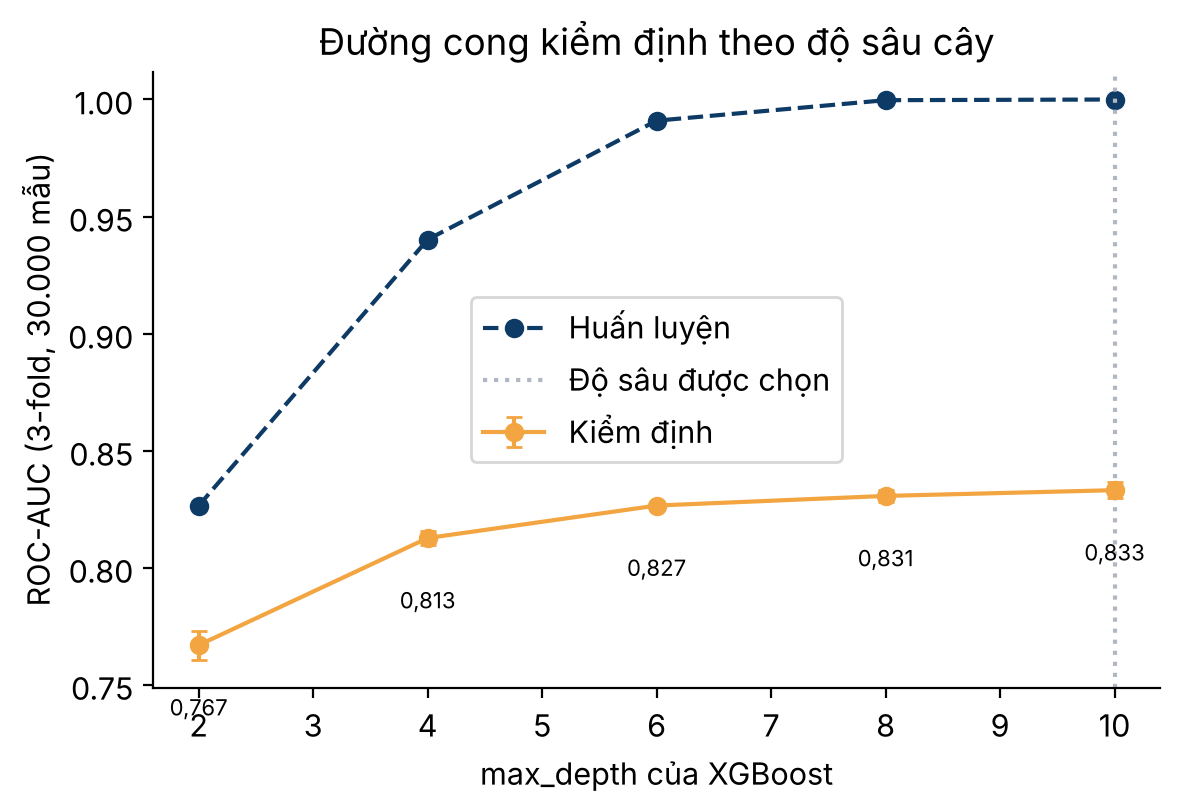
\includegraphics[width=0.7\textwidth]{fig15_duong_cong_kiem_dinh.png}
  \caption{Đường cong kiểm định theo độ sâu cây của XGBoost (các siêu tham số khác giữ ở giá trị tối ưu)}
  \label{fig:duongcongkiemdinh}
\end{figure}

\textit{Nhận xét} (Hình~\ref{fig:duongcongkiemdinh}): ROC-AUC kiểm định tăng nhanh
khi độ sâu tăng từ 2 (0,767) đến 6 (0,827), sau đó tăng chậm (0,831 ở độ sâu 8,
0,833 ở độ sâu 10), trong khi ROC-AUC huấn luyện chạm 1,0 từ độ sâu 8. Như vậy
tương tác thuốc cần các tổ hợp nhiều mảnh cấu trúc (cây sâu), và điều chuẩn L2
mạnh cùng việc lấy mẫu đặc trưng giữ cho mô hình không bị quá khớp dù điểm huấn
luyện rất cao. Độ sâu tối ưu nằm ở biên không gian tìm kiếm, nên vẫn có thể thử
độ sâu lớn hơn ở các nghiên cứu sau.

\subsection{Thử nghiệm thuật toán mới và phương pháp tổ hợp}
\begin{itemize}
  \item Extra Trees (300 cây, \texttt{max\_features = sqrt}, biểu diễn ghép
        nối): ngưỡng chia chọn ngẫu nhiên giúp các cây khác nhau hơn rừng ngẫu nhiên.
  \item Soft Voting RF + XGBoost: lấy trung bình xác suất của Random Forest
        và XGBoost đã tối ưu, trọng số bằng nhau. Trong kiểm định chéo, xác suất
        ngoài fold của hai mô hình được lấy trung bình trên đúng từng fold, nên
        không cần huấn luyện thêm và không rò rỉ dữ liệu.
\end{itemize}
Kết quả của hai phương pháp này được đưa vào bảng so sánh chung ở
Mục~\ref{sec:sosanh}.

\section{So sánh đối sánh công bằng giữa các thuật toán}
\label{sec:sosanh}

\begin{table}[H]
  \centering
  \caption{So sánh trước -- sau cải tiến (kiểm định chéo 5-fold trên cùng 80.000 mẫu, cùng cách chia)}
  \label{tab:ablation}
  \footnotesize\setlength{\tabcolsep}{4pt}
  \begin{tabular}{llccccr}
    \toprule
    & \textbf{Cấu hình} & \textbf{ROC-AUC} & \textbf{F1} & \textbf{Recall} & \textbf{AUC train} & \textbf{Fit (s)} \\
    \midrule
    \multirow{4}{*}{XGBoost}
      & Ban đầu (ghép nối, mặc định) & 0,847 $\pm$ 0,002 & 0,773 & 0,799 & 0,928 & 45 \\
      & + biểu diễn đối xứng & 0,853 $\pm$ 0,003 & 0,776 & 0,796 & 0,939 & 24 \\
      & + Morgan đếm, hóa lý & 0,854 $\pm$ 0,002 & 0,779 & 0,803 & 0,935 & 33 \\
      & + tối ưu siêu tham số & 0,881 $\pm$ 0,001 & 0,805 & 0,824 & 0,998 & 59 \\
    \midrule
    \multirow{2}{*}{Random Forest}
      & Ban đầu (ghép nối, mặc định) & 0,858 $\pm$ 0,002 & 0,783 & 0,809 & 1,000 & 76 \\
      & + tối ưu siêu tham số & 0,859 $\pm$ 0,002 & 0,786 & 0,815 & 1,000 & 477 \\
    \midrule
    Mới & Extra Trees (ghép nối) & 0,863 $\pm$ 0,002 & 0,790 & 0,817 & 1,000 & 137 \\
    Tổ hợp & Voting RF + XGBoost tối ưu & 0,885 $\pm$ 0,002 & 0,810 & 0,833 & -- & 537 \\
    \midrule
    Cơ sở & Logistic Regression (ghép nối) & 0,807 $\pm$ 0,003 & 0,739 & 0,756 & 0,837 & 23 \\
          & Dummy & 0,500 & 0,000 & 0,000 & 0,500 & 0 \\
    \bottomrule
  \end{tabular}
\end{table}

\begin{figure}[H]
  \centering
  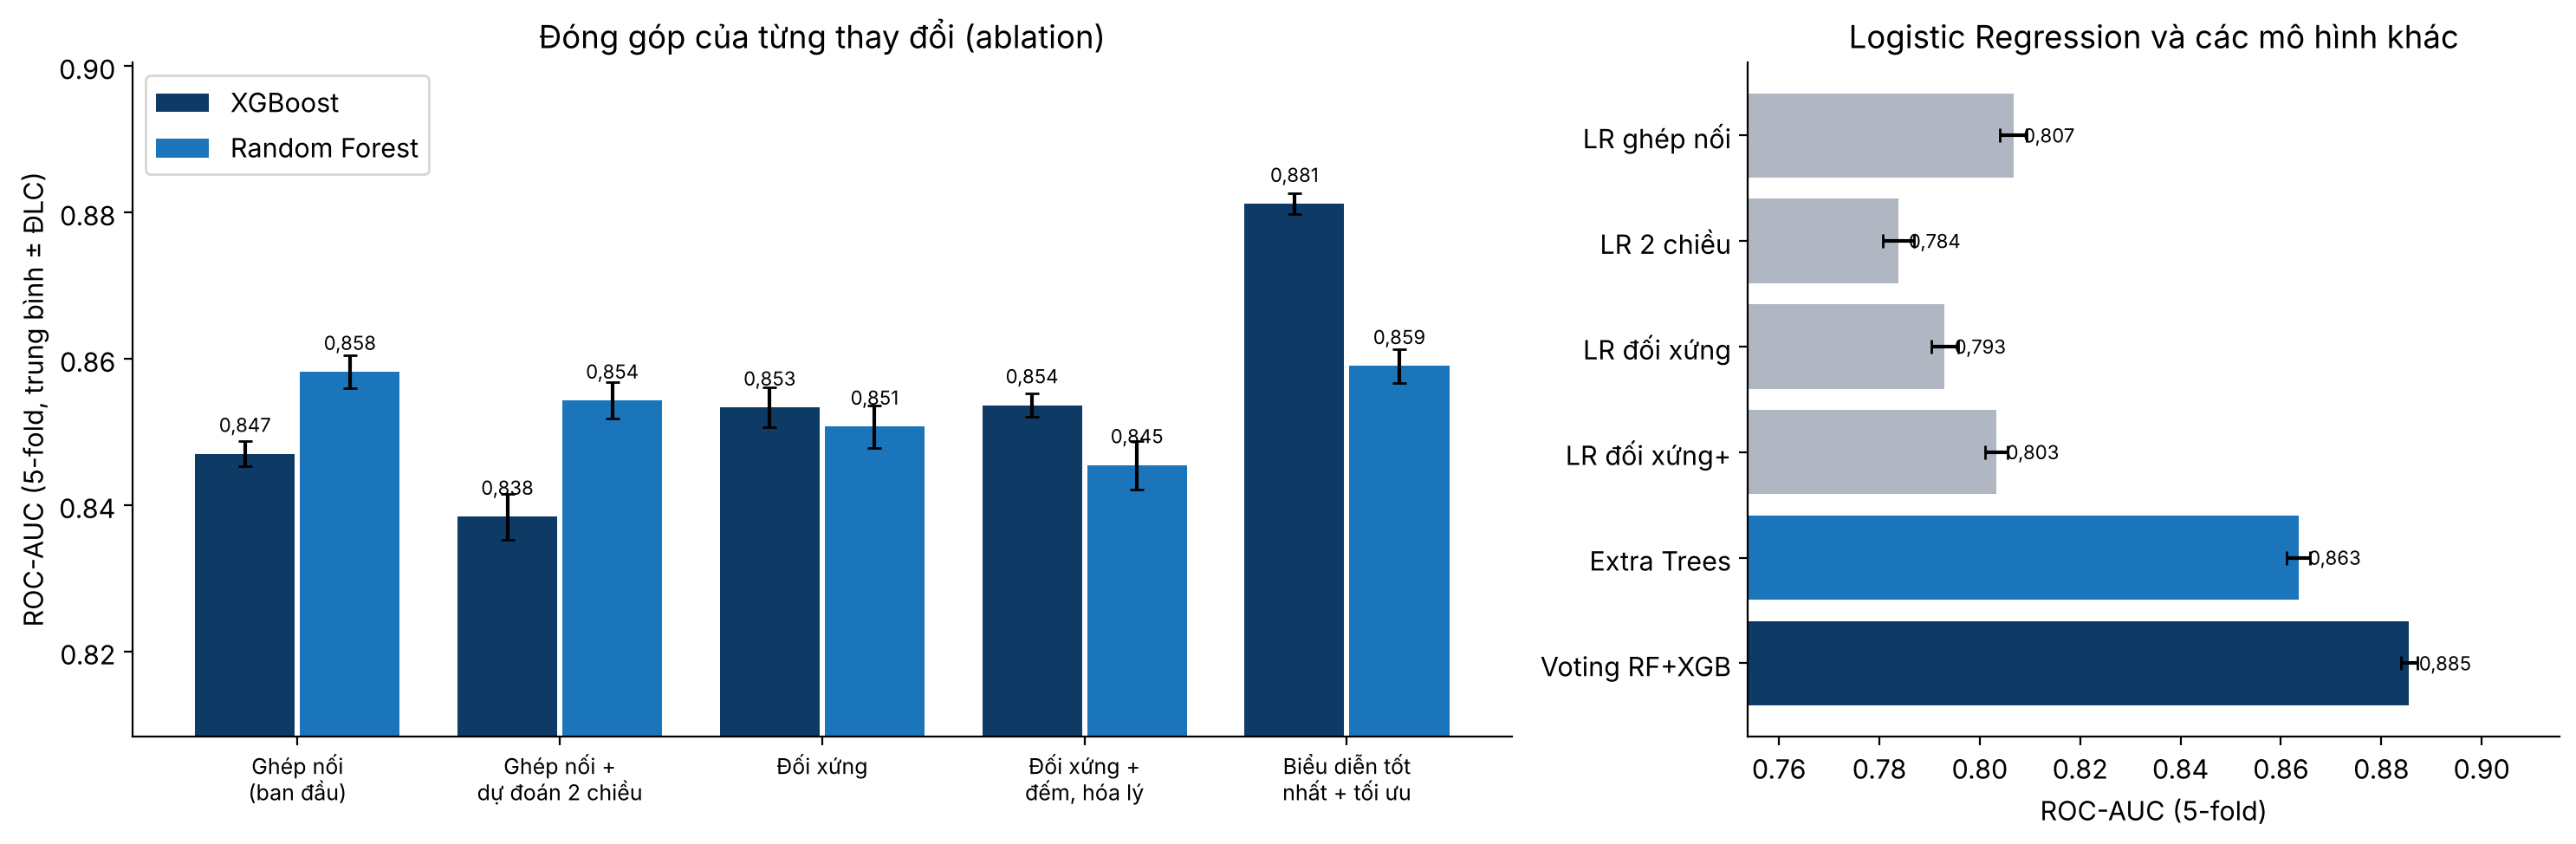
\includegraphics[width=\textwidth]{fig16_ablation.png}
  \caption{Đóng góp của từng thay đổi (trái) và kết quả của Logistic Regression, Extra Trees, Soft Voting (phải); thanh lỗi là độ lệch chuẩn qua 5 fold}
  \label{fig:ablation}
\end{figure}

\textit{Nhận xét} (Bảng~\ref{tab:ablation}, Hình~\ref{fig:ablation}):
\begin{itemize}
  \item Tối ưu siêu tham số đóng góp nhiều nhất cho XGBoost: +0,027 ROC-AUC
        (0,854 $\rightarrow$ 0,881) và +0,026 F1, lớn hơn 10 lần độ lệch chuẩn
        giữa các fold. Thay đổi biểu diễn đóng góp +0,006. Tổng cộng XGBoost tăng từ
        0,847 lên 0,881 và vượt Random Forest.
  \item Random Forest gần như không cải thiện khi tối ưu (+0,001) dù thời
        gian huấn luyện tăng hơn 6 lần (500 cây, xét 10\% đặc trưng mỗi nút). Cây của
        RF đã phát triển hết độ sâu nên điểm huấn luyện luôn bằng 1; các siêu tham số
        thử nghiệm không làm thay đổi bản chất này.
  \item Extra Trees (thuật toán mới) tốt hơn RF 0,005 và nhanh hơn RF đã
        tối ưu 3,5 lần.
  \item Soft Voting cho kết quả tốt nhất (ROC-AUC 0,885, F1 0,810, Recall
        0,833) và ổn định nhất (độ lệch chuẩn F1 0,001). RF (bagging, cây sâu) và
        XGBoost (boosting, có điều chuẩn) mắc lỗi khác nhau, nên lấy trung bình xác
        suất bù trừ được một phần lỗi của nhau.
  \item Các cải tiến đều so sánh trên cùng dữ liệu, cùng 5 fold và cùng chỉ số; từng
        dòng chỉ thay đổi một yếu tố so với dòng trên (ablation).
\end{itemize}

\section{Khả năng tổng quát hóa và ảnh hưởng của cách lấy mẫu âm}
\label{sec:tongquat}

\subsection{Kết quả trên tập kiểm tra giữ lại}
Các mô hình được huấn luyện lại trên toàn bộ 80.000 mẫu với cấu hình đã chọn, rồi
đánh giá một lần trên 20.000 cặp của tập kiểm tra (Bảng~\ref{tab:test3}).

\begin{table}[H]
  \centering
  \caption{Kết quả trên tập kiểm tra giữ lại và so sánh với kiểm định chéo}
  \label{tab:test3}
  \footnotesize\setlength{\tabcolsep}{4pt}
  \begin{tabular}{lcccccc}
    \toprule
    \textbf{Mô hình} & \textbf{ROC-AUC CV} & \textbf{ROC-AUC test} & \textbf{F1} & \textbf{Recall} & \textbf{Precision} & \textbf{Accuracy} \\
    \midrule
    XGBoost ban đầu & 0,847 & 0,853 & 0,779 & 0,810 & 0,751 & 0,771 \\
    Random Forest ban đầu & 0,858 & 0,865 & 0,789 & 0,822 & 0,759 & 0,780 \\
    XGBoost tối ưu & 0,881 & 0,887 & 0,810 & 0,834 & 0,789 & 0,805 \\
    Random Forest tối ưu & 0,859 & 0,865 & 0,791 & 0,823 & 0,761 & 0,782 \\
    \textbf{Voting RF + XGBoost} & \textbf{0,885} & \textbf{0,891} & \textbf{0,816} & \textbf{0,841} & \textbf{0,792} & \textbf{0,810} \\
    \bottomrule
  \end{tabular}
\end{table}

\begin{figure}[H]
  \centering
  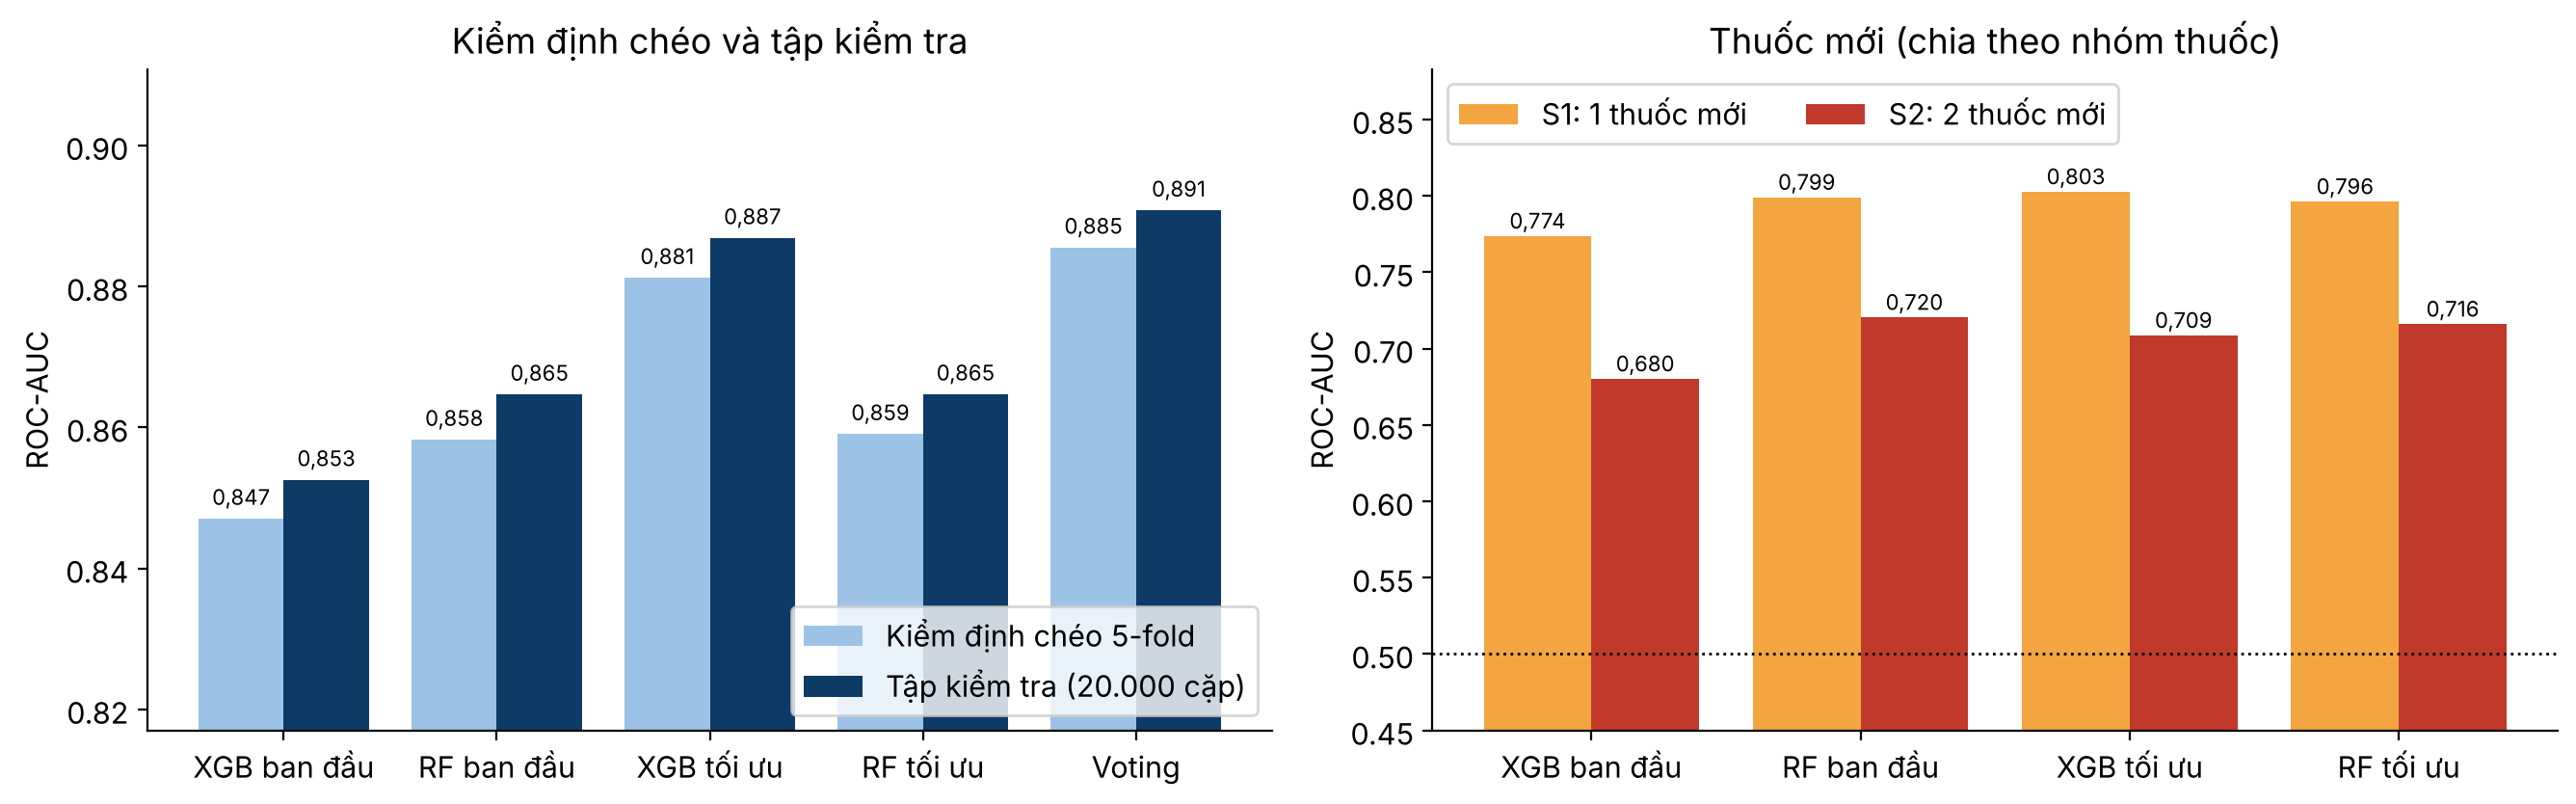
\includegraphics[width=\textwidth]{fig17_tong_quat_hoa.png}
  \caption{ROC-AUC kiểm định chéo và tập kiểm tra (trái); ROC-AUC trên thuốc mới S1, S2 (phải)}
  \label{fig:tongquat}
\end{figure}

\textit{Nhận xét} (Bảng~\ref{tab:test3}, Hình~\ref{fig:tongquat}):
\begin{itemize}
  \item Điểm trên tập kiểm tra cao hơn kiểm định chéo một chút (0,005--0,007) ở mọi
        mô hình, vì mô hình cuối được học trên 80.000 mẫu thay vì 64.000 mẫu của mỗi
        fold (đường cong học tập ở Hình~\ref{fig:duongconghoc} vẫn đang đi lên). Thứ
        hạng các mô hình giữ nguyên, không có dấu hiệu chọn mô hình ``ăn may'' theo
        kiểm định chéo.
  \item Mô hình Voting ổn định qua các fold: ROC-AUC từ 0,884 đến 0,888, F1 từ
        0,808 đến 0,812 (độ lệch chuẩn 0,002 và 0,001).
  \item Trên tập kiểm tra, Voting phát hiện 84,1\% số cặp có tương tác (Recall) với
        độ chính xác cảnh báo 79,2\%, đạt cả ba mục tiêu ở Bảng~\ref{tab:muctieu}:
        ROC-AUC 0,891 $\geq 0{,}85$, F1 0,816 $\geq 0{,}80$, Recall 0,841 $\geq 0{,}80$.
\end{itemize}

\subsection{Khả năng tổng quát hóa cho thuốc mới}
Khi huấn luyện chỉ trên các cặp gồm thuốc đã biết (63.756 cặp) và đánh giá trên cặp
có thuốc mới, XGBoost tối ưu đạt ROC-AUC 0,803 (S1, một thuốc mới) và 0,709 (S2, hai
thuốc mới), tốt hơn XGBoost ban đầu (0,774 và 0,680). Random Forest tối ưu đạt 0,796
và 0,716, gần như không đổi so với ban đầu (0,799 và 0,720). Mục tiêu ROC-AUC
$\geq 0{,}75$ với một thuốc mới đạt được; với hai thuốc mới hiệu năng còn thấp
(khoảng 0,71) -- đây là giới hạn của cách tiếp cận chỉ dùng cấu trúc hóa học.

\subsection{Ảnh hưởng của cách lấy mẫu âm theo bậc}
\begin{figure}[H]
  \centering
  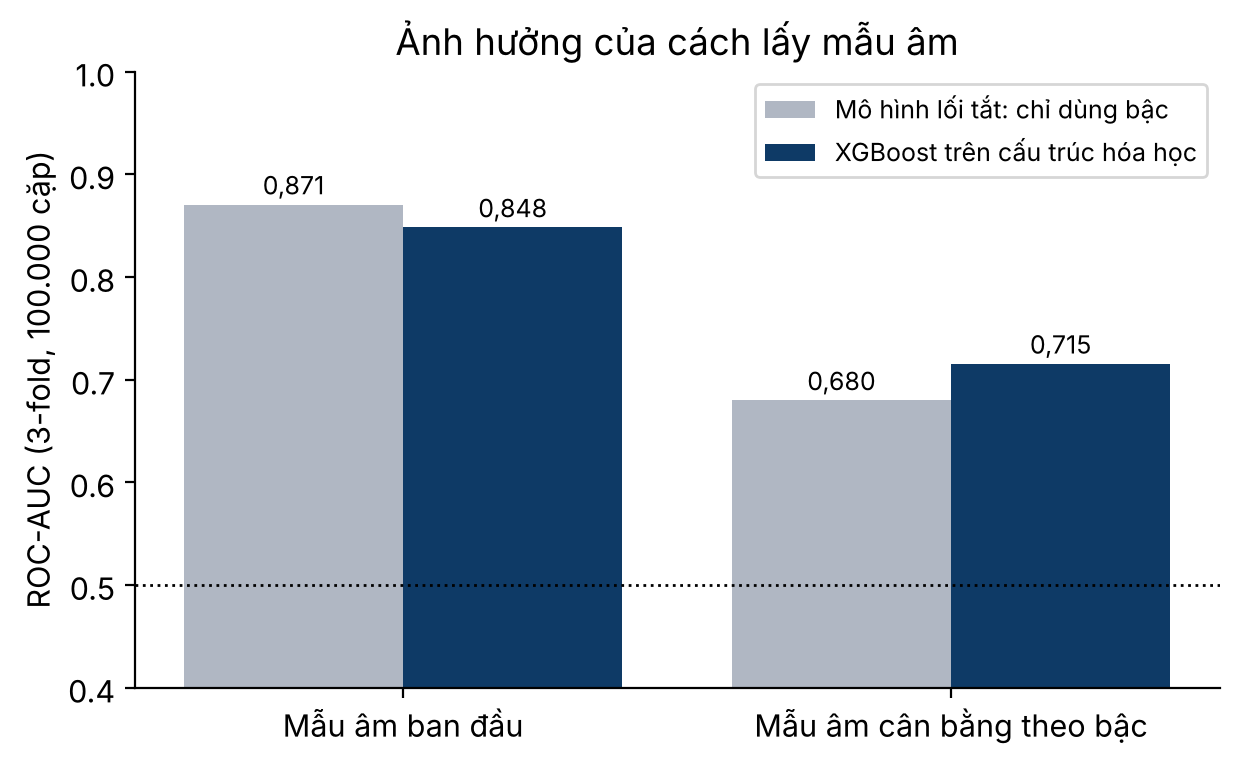
\includegraphics[width=0.68\textwidth]{fig18_lay_mau_am_theo_bac.png}
  \caption{ROC-AUC (kiểm định chéo 3-fold, 100.000 cặp) của mô hình chỉ dùng bậc và XGBoost trên cấu trúc, với hai cách lấy mẫu âm}
  \label{fig:laymauam}
\end{figure}

\textit{Nhận xét} (Hình~\ref{fig:laymauam}): với mẫu âm ban đầu, một mô hình chỉ
dùng bậc của hai thuốc (không có thông tin cấu trúc) đã đạt ROC-AUC 0,871, cao hơn
XGBoost trên cấu trúc (0,848). Khi lấy lại mẫu âm sao cho mỗi thuốc xuất hiện trong
mẫu âm với tần suất như trong mẫu dương, mô hình ``lối tắt'' chỉ còn 0,680, còn
XGBoost giảm xuống 0,715 nhưng vượt mô hình lối tắt. Như vậy:
\begin{itemize}
  \item một phần đáng kể hiệu năng trong bảng kết quả đến từ độ phổ biến của thuốc
        do cách lấy mẫu âm, không phải từ quan hệ cấu trúc giữa hai thuốc;
  \item thông tin cấu trúc vẫn có giá trị thật (XGBoost $>$ mô hình lối tắt khi đã
        loại thiên lệch), nhưng bài toán khó hơn nhiều so với con số 0,89;
  \item kết quả của các nghiên cứu dùng mẫu âm ngẫu nhiên (kể cả Ran \textit{et al.})
        nên được đọc với lưu ý này. Nhóm giữ cách lấy mẫu âm ban đầu cho bảng kết quả
        chính để thống nhất với Bài kiểm tra 1 và các nghiên cứu trước, và báo cáo
        thí nghiệm này như một giới hạn của bài toán.
\end{itemize}

\section{Đánh giá và kết luận}
\label{sec:chonmodel}

\subsection{Giải thích vì sao cải tiến có hoặc không hiệu quả}
\begin{itemize}
  \item Tối ưu XGBoost hiệu quả vì cấu hình mặc định (độ sâu 6) quá nông so
        với bài toán: tương tác thuốc cần tổ hợp nhiều mảnh cấu trúc. Cấu hình tối ưu
        dùng cây sâu 10 để biểu diễn tổ hợp này, đồng thời điều chuẩn L2 mạnh
        (\texttt{reg\_lambda} $= 9{,}1$), \texttt{min\_child\_weight} $= 5$ và chỉ lấy
        1/3 số đặc trưng mỗi cây để không quá khớp (Hình~\ref{fig:duongcongkiemdinh}).
  \item Tối ưu RF không hiệu quả vì RF giảm phương sai bằng trung bình nhiều
        cây chứ không bằng điều chuẩn từng cây; tăng số cây từ 300 lên 500 hay đổi số
        đặc trưng mỗi nút chỉ thay đổi rất ít khi số cây đã đủ lớn.
  \item Dự đoán hai chiều không hiệu quả vì mô hình chưa từng thấy thứ tự
        ngược khi học; biểu diễn đối xứng chỉ có lợi cho mô hình nông
        (XGBoost) mà bất lợi cho mô hình khai thác được thông tin vị trí (RF).
  \item Soft Voting hiệu quả vì hai mô hình thành phần đủ tốt và có kiểu lỗi
        khác nhau (bagging/boosting, hai biểu diễn đặc trưng khác nhau).
\end{itemize}

\subsection{Lựa chọn mô hình cuối}
\begin{table}[H]
  \centering
  \caption{Đánh đổi giữa các mô hình ứng viên}
  \label{tab:chonmohinh}
  \small
  \begin{tabularx}{\textwidth}{l c c c >{\raggedright\arraybackslash}X}
    \toprule
    \textbf{Mô hình} & \textbf{ROC-AUC CV} & \textbf{ĐLC} & \textbf{Fit (s/fold)} & \textbf{Khả năng diễn giải, triển khai} \\
    \midrule
    Voting RF + XGBoost & 0,885 & 0,002 & 537 & Tốt nhất, ổn định nhất; mô hình lớn (RF 500 cây sâu), chậm hơn \\
    XGBoost tối ưu & 0,881 & 0,001 & 59 & Gần bằng Voting, nhanh gấp 9 lần, gọn; có độ quan trọng đặc trưng \\
    Extra Trees & 0,863 & 0,002 & 137 & Không cần tối ưu, nhưng kém hơn rõ rệt \\
    Random Forest tối ưu & 0,859 & 0,002 & 477 & Chậm, tối ưu gần như không cải thiện \\
    \bottomrule
  \end{tabularx}
\end{table}

Nhóm chọn Soft Voting RF + XGBoost làm mô hình cuối vì có ROC-AUC, F1,
Recall cao nhất cả trong kiểm định chéo và trên tập kiểm tra, và ổn định nhất qua
các fold; với ứng dụng sàng lọc tương tác thuốc, mô hình được huấn luyện một lần
nên thời gian huấn luyện lớn hơn là chấp nhận được. Khi cần mô hình gọn và nhanh
(ví dụ tích hợp vào ứng dụng), XGBoost tối ưu là phương án thay thế: chỉ
kém 0,004 ROC-AUC nhưng nhanh gấp 9 lần.

% =====================================================================
%  KẾT LUẬN
% =====================================================================
\unnumberedchapter{KẾT LUẬN VÀ HƯỚNG PHÁT TRIỂN}

\section*{1. Kết quả đạt được}
\begin{itemize}
  \item Phát biểu bài toán phân loại nhị phân trên cặp thuốc, xây dựng bộ dữ liệu
        100.000 cặp sạch từ DrugBank 5.1 kèm từ điển dữ liệu, khảo sát, xử lý chất
        lượng dữ liệu và chuẩn bị dữ liệu không rò rỉ (Bài kiểm tra 1).
  \item Huấn luyện và so sánh Logistic Regression, Random Forest, XGBoost, SVM với mô
        hình cơ sở bằng kiểm định chéo 5-fold và tập kiểm tra giữ lại; Random Forest
        tốt nhất ở cấu hình ban đầu (ROC-AUC 0,858); phân tích lỗi theo bậc thuốc và
        độ tương đồng cấu trúc (Bài kiểm tra 2).
  \item Phân tích hạn chế dựa trên bằng chứng, thử ba cách biểu diễn cặp thuốc, tối
        ưu siêu tham số bằng Random Search, thử Extra Trees và Soft Voting. Mô hình
        cuối (Voting RF + XGBoost) đạt ROC-AUC 0,891, F1 0,816, Recall 0,841 trên tập
        kiểm tra, đạt cả ba mục tiêu; với một thuốc mới, XGBoost tối ưu đạt ROC-AUC
        0,803 (Bài kiểm tra 3).
\end{itemize}

\section*{2. Hạn chế}
\begin{itemize}
  \item Mẫu âm là các cặp chưa ghi nhận tương tác, có thể lẫn tương tác có
        thật chưa được phát hiện. Khi lấy mẫu âm cân bằng theo bậc, ROC-AUC của
        XGBoost giảm từ 0,848 xuống 0,715: một phần hiệu năng đến từ độ phổ biến của
        thuốc chứ không phải từ cấu trúc.
  \item Hiệu năng giảm mạnh khi cả hai thuốc đều mới (ROC-AUC khoảng 0,71).
  \item Biểu diễn ghép nối phụ thuộc thứ tự hai thuốc; tăng cường dữ liệu bằng nhân
        đôi thứ tự chưa thực hiện được do giới hạn bộ nhớ (8~GB RAM).
  \item Việc tìm siêu tham số chạy trên tập con 30.000 mẫu với số cấu hình nhỏ (6--10)
        do giới hạn thời gian; độ sâu tối ưu của XGBoost nằm ở biên không gian tìm kiếm.
\end{itemize}

\section*{3. Hướng phát triển}
\begin{itemize}
  \item Dùng cách lấy mẫu âm cân bằng theo bậc (hoặc đánh giá trên cả hai cách) làm
        chuẩn đánh giá chính; huấn luyện trên cả hai thứ tự của cặp khi có máy mạnh hơn.
  \item Mở rộng không gian tìm kiếm (độ sâu lớn hơn, nhiều cấu hình hơn, Bayesian
        Optimization) và thử LightGBM, Stacking.
  \item Bổ sung đặc trưng sinh học như protein đích, enzyme chuyển hóa, chất vận
        chuyển của thuốc để cải thiện dự đoán cho thuốc mới; mở rộng sang dự đoán
        loại tương tác.
\end{itemize}

% =====================================================================
%  TÀI LIỆU THAM KHẢO
% =====================================================================

% =====================================================================
%  TÀI LIỆU THAM KHẢO
% =====================================================================
\begin{thebibliography}{99}
\setlength{\itemsep}{2pt}

\bibitem{breiman2001}
L.~Breiman (2001), ``Random forests'', \textit{Machine Learning}, vol.~45,
no.~1, pp.~5--32.

\bibitem{chen2016}
T.~Chen, C.~Guestrin (2016), ``XGBoost: A scalable tree boosting system'',
in \textit{Proceedings of the 22nd ACM SIGKDD International Conference on
Knowledge Discovery and Data Mining}, pp.~785--794.

\bibitem{cheng2014}
F.~Cheng, Z.~Zhao (2014), ``Machine learning-based prediction of drug--drug
interactions by integrating drug phenotypic, therapeutic, chemical, and genomic
properties'', \textit{Journal of the American Medical Informatics Association},
vol.~21, no.~e2, pp.~e278--e286.

\bibitem{cortes1995}
C.~Cortes, V.~Vapnik (1995), ``Support-vector networks'', \textit{Machine
Learning}, vol.~20, no.~3, pp.~273--297.

\bibitem{deng2020}
Y.~Deng, X.~Xu, Y.~Qiu, J.~Xia, W.~Zhang, S.~Liu (2020), ``A multimodal deep
learning framework for predicting drug--drug interaction events'',
\textit{Bioinformatics}, vol.~36, no.~15, pp.~4316--4322.

\bibitem{durant2002}
J.~L.~Durant, B.~A.~Leland, D.~R.~Henry, J.~G.~Nourse (2002), ``Reoptimization
of MDL keys for use in drug discovery'', \textit{Journal of Chemical Information
and Computer Sciences}, vol.~42, no.~6, pp.~1273--1280.

\bibitem{geurts2006}
P.~Geurts, D.~Ernst, L.~Wehenkel (2006), ``Extremely randomized trees'',
\textit{Machine Learning}, vol.~63, no.~1, pp.~3--42.

\bibitem{gottlieb2012}
A.~Gottlieb, G.~Y.~Stein, Y.~Oron, E.~Ruppin, R.~Sharan (2012), ``INDI: a
computational framework for inferring drug interactions and their associated
recommendations'', \textit{Molecular Systems Biology}, vol.~8, Article 592.

\bibitem{rdkit}
G.~Landrum, ``RDKit: Open-source cheminformatics'', \url{https://www.rdkit.org}.

\bibitem{lin2020}
X.~Lin, Z.~Quan, Z.-J.~Wang, T.~Ma, X.~Zeng (2020), ``KGNN: Knowledge graph
neural network for drug--drug interaction prediction'', in \textit{Proceedings
of the Twenty-Ninth International Joint Conference on Artificial Intelligence
(IJCAI-20)}, pp.~2739--2745.

\bibitem{nyamabo2021}
A.~K.~Nyamabo, H.~Yu, J.-Y.~Shi (2021), ``SSI--DDI: substructure--substructure
interactions for drug--drug interaction prediction'', \textit{Briefings in
Bioinformatics}, vol.~22, no.~6, bbab133.

\bibitem{pedregosa2011}
F.~Pedregosa \textit{et al.} (2011), ``Scikit-learn: Machine learning in
Python'', \textit{Journal of Machine Learning Research}, vol.~12,
pp.~2825--2830.

\bibitem{ran2022}
B.~Ran, L.~Chen, M.~Li, Y.~Han, Q.~Dai (2022), ``Drug-drug interactions
prediction using fingerprint only'', \textit{Computational and Mathematical
Methods in Medicine}, vol.~2022, Article ID 7818480.

\bibitem{rogers2010}
D.~Rogers, M.~Hahn (2010), ``Extended-connectivity fingerprints'',
\textit{Journal of Chemical Information and Modeling}, vol.~50, no.~5,
pp.~742--754.

\bibitem{ryu2018}
J.~Y.~Ryu, H.~U.~Kim, S.~Y.~Lee (2018), ``Deep learning improves prediction of
drug--drug and drug--food interactions'', \textit{Proceedings of the National
Academy of Sciences}, vol.~115, no.~18, pp.~E4304--E4311.

\bibitem{vilar2012}
S.~Vilar, R.~Harpaz, E.~Uriarte, L.~Santana, R.~Rabadan, C.~Friedman (2012),
``Drug--drug interaction through molecular structure similarity analysis'',
\textit{Journal of the American Medical Informatics Association}, vol.~19,
no.~6, pp.~1066--1074.

\bibitem{weininger1988}
D.~Weininger (1988), ``SMILES, a chemical language and information system.
1: Introduction to methodology and encoding rules'', \textit{Journal of Chemical
Information and Computer Sciences}, vol.~28, no.~1, pp.~31--36.

\bibitem{wishart2018}
D.~S.~Wishart \textit{et al.} (2018), ``DrugBank 5.0: a major update to the
DrugBank database for 2018'', \textit{Nucleic Acids Research}, vol.~46,
no.~D1, pp.~D1074--D1082.

\bibitem{zhang2017}
W.~Zhang, Y.~Chen, F.~Liu, F.~Luo, G.~Tian, X.~Li (2017), ``Predicting
potential drug-drug interactions by integrating chemical, biological,
phenotypic and network data'', \textit{BMC Bioinformatics}, vol.~18,
Article 18.

\bibitem{zitnik2018}
M.~Zitnik, M.~Agrawal, J.~Leskovec (2018), ``Modeling polypharmacy side effects
with graph convolutional networks'', \textit{Bioinformatics}, vol.~34, no.~13,
pp.~i457--i466.

\end{thebibliography}


\end{document}
